\documentclass{book}

\usepackage[hyphens]{url}
\usepackage[utf8]{inputenc}
\usepackage{csquotes}
\usepackage{fontspec}
\usepackage{graphicx}
\graphicspath{ {./images/} }
\usepackage{listings}
\usepackage{authblk}
\usepackage[normalem]{ulem}
\usepackage[bottom]{footmisc}
\usepackage{hyperref}
\usepackage{float}
\usepackage[leqno]{amsmath}
\usepackage[]{natbib}

\usepackage{etoolbox}
\AtBeginEnvironment{quote}{\itshape}

\usepackage[]{minted}
\usemintedstyle{trac}
\usepackage{caption}
\newenvironment{code}{\captionsetup{type=listing}}{}

\graphicspath{ {./images/} }

\defaultfontfeatures{Mapping=tex-text,Scale=1.00}
\setmainfont{Bespoke Serif}
\setmonofont{IBM Plex Mono}
\linespread{1.50}
\sloppy

\lstset{
    basicstyle=\footnotesize\ttfamily,
    breaklines=true,
    frame=single,
    captionpos=b,
    belowcaptionskip=2em,
    aboveskip=2em
}

\begin{document}
\title{The role of Aesthetics in the Understandings of Source code}
\author{Pierre Depaz\\under the direction of Alexandre Gefen (Paris-3)\\and Nick Montfort (MIT)}
\affil{ED120 - THALIM}
\date{last updated - 3.12.2022}
\maketitle

\chapter{Introduction}
\label{chap:introduction}

This thesis is an inquiry into the formal manifestations of source code, into how particular configurations of lines of code allow for aesthetic judgments and on the purposes that such configurations serve. The implications of this inquiry will lead us to consider the different ways in which people read and the different ways in which source code can be represented, depending on what it aims at accomplishing, and on the contexts in which it operates.
This study on source code involves the different groups of people which read and write it, the purposes for which they write it, the programming languages they use to write it, and the natural language they use to speak about it. Most importantly, this thesis focuses on source code as a material and linguistic manifestation of a larger digital ecosystem of software and hardware to which it belongs. Since source code is only one component of code, as we will see below, this thesis also aims at studying the reality of written code, rather than its conceptual interpretations.

Starting from pieces of source code, this thesis will aim at assessing what programmers have to say about it, and attempt to identify how one or more specific \emph{aesthetic fields} are used to refer to it. This aim depends on two facts: first, source code is a medium for expression, both to express the programmer's intent to the computer \citep{dijkstra_craftsman_1982} and the programmer's intent to another programmer \citep{abelson_structure_1979}—here we also consider the same individual at two different points in time as two different programmers. Second, source code is a relatively new medium, compared to, say, paint or mechanics. As such, the development and solidification of aesthetic practices—that is, of ways of doing which do not find their immediate justification in a practical accomplishment—is an ongoing research project in computer science, software development and the digital humanities. Formal judgments of source code are therefore existing and well-documented, and are related to a need for expressiveness, as we will see in chapter 2, but their formalization is still an ongoing process.

Source code thus can be written in a way makes it subject to aesthetic judgments by programmers; that is, code \emph{has} aesthetics, but it is unclear exactly \emph{which} aesthetics. Indeed, these aesthetic judgments as they exist today rely on different domains to assess source code, as a means to grasp the cognitive object that is software. These draw from metaphors ranging from literature, architecture, mathematics and engineering. And yet, source code, while related to all of these, isn't exactly any of the them. Like the story of the seven blind men and the elephant \citep{chun_sourcery_2008}, each of these domains touch on some specific aspect of the nature of code, but none of them are sufficient to entirely provide a solid basis for the aesthetic judgments of source code. It is at the crossroads of these domains that this thesis locates its work.

The examination of source code, and of the discourses around source code will integrate both the diversity of ways in which source code can exist, and the invariant aspects which underline all diverse approaches of source code. Particularly, we will see how each groups of practicionners tend to deploy references to underlying, systematic conceptual metaphors drawing from the domains above, but also how these references overlap across groups. The point of overlap, as we will demontrate, is that of \emph{using a formal linguistic system to communicate the understanding of complex cognitive structures}. Through an interdisciplinary approach, we attempt to connect this formal symbol system to the broader role of aesthetics as a cognitive mechanism to deal with complexity.

The rest of this introduction will consist in establishing a more complete view of the context in which this research takes place, from computer science to digital humanities and science and technology studies. With this context at hand, we will proceed to highlight the specific problems which will be tackled regarding the current place of aesthetics in source code. After outlining our methodology and the theoretical frameworks which will be mobilized throughout this study, we will sketch out how the different chapters of this thesis will attempt at providing some responses to our research questions.

\section{Context}
\label{sec:context}

\subsection{The research territory: code}
\label{subsec:research-territory}

Most of our modern infrastructure depends, to a more or less dramatic extent, on software systems \citep{kitchin_code_2011}, from commercial spaces to classrooms, transport systems to cultural institutions, scientific production and entertainment products. Software regulates and automates the information stores, exchanges and creation which compose each of these domains of human activities.  The complex processes are described in what is called source code, a vast and invisible set of texts. The number of lines of code involved in running these processes is hard to estimate; one can only rely on disclosures from companies, and publicly available repositories. To give an order of magnitude, all of Google's services amounted to over two billions source lines of code (SLOC) \citep{scale_why_2015}, while the 2005 release of the OSX operating system comprised 86 millions lines of code, and while the version 1.0 of the Linux kernel (an operating system which powers most of the internet and specialized computation) totalled over 175,000 SLOC, version 4.1 jumped to over 19.5 million lines of code in the span of twenty years \citep{wikipedia_linux_2021}.

Given such a large quantity of textual mass, one might wonder: who reads this code? To answer this question, we must start diving a bit deeper into what source code really is.

Source code consists in a series of instructions, composed in a particular programming language, which is then processed by a computer in order to be executed. For instance, using the language called Python, the source code in \ref{code:simple_example} consists in telling the computer to store two numbers in what are called \emph{variables}, then proceeds with describing the \emph{procedure} for adding the double of the first terms to the second term, and concludes in actually executing the above procedure.

\begin{listing}
    \inputminted{python}{./corpus/simple.py}
    \caption{Example of the basic elements of a computer program, written in Python}
    \label{code:simple_example}
\end{listing}

Given this particular piece of source code, the computer will output the number \lstinline{14} as the result of the operation \lstinline{(4 * 2) + 6}. In this sense, then, source code is the requirement for software to exist: since computers are procedural machines, acting upon themselves and upon the world, they need a specification of what to do, and source code provides such a specification. In this sense, computers are the main "readership" of source code.

However, it is  also a by-product of software, since it is no longer required once the computer has processed and stored it into a \emph{binary} representation, a series of 0s and 1s which represent the successive states that the computer has to go through in order to perform the action that was described in the source code. \emph{Binary code} is what most of the individuals who interact with computers deal with, in the form of packaged applications, such as a media player or a web browser. They (almost) never have to inquire about, or read, such source code. In this sense, then, source code only matters until it gets processed by a computer, through which it realizes its intended function.

From another perspective, source code isn't just about telling computers what to do, but also a key component of a particular economy: that of software development. Software developers are the ones who write the source code and this process is first and foremost a collaborative endeavour. Software developers write code in successive steps, because they add features over time, or they fix errors that have shown up in their software, or they decide to rewrite parts of the source code based on new ideas, skills or preferences. In this case, source code is not used to communicate to the computer what it does, but to other software developers what the \emph{intent} of the software is. Source code is then the locus of human, collaborative work; it represents iterations of ideas, formalization of processes and approaches to problem-solving. As Harold Abelson puts it,

\begin{quote}
    "Programs must be written for people to read, and only incidentally for machines to execute." \citep{abelson_structure_1979}.
\end{quote}


Official definitions of source code straddle this line between the first role of source code (as instructions to a computer) and the second role of source code (as indications to a programmer). For instance, a definition within the context of the Institute of Electrical and Electronics Engineering (IEEE) considers source code \emph{any fully executable description of a software system, which therefore includes various representations of this description, from machine code to high-level languages and graphical representations using visual programming languages} \citep{harman_why_2010}. This definition focuses on the ability of code to be processed by a machine, and mentions little about its readability (i.e. processability by other humans).

On the other hand, the definition of source code provided by the Linux Information Project\footnote{https://linfo.org/sourcecode.html} focuses on source code as \emph{the version of software as it is originally written (i.e. typed into a computer), by a human in plain text (i.e. human-readable, alphanumeric characters).} \citep{linuxinformationproject_source_2004}. The emphasis here is on source code as the support of human activity, as software developers need to understand the pieces of code that they are creating, or modifying. Source code thus has two kinds of readabilities: a computer one, which is geared towards the correct execution of the program, and a human one, which is geared towards the correct understanding of the program. In the lineage of this human-readability, we can point to the Free Software Foundation's equation of the free circulation and publication of source code with the free circulation of publication of ideas. Particularly, Freedom 1 (\emph{The freedom to study how the program works, and adapt it to your needs}) and Freedom 2 (\emph{The freedom to improve the program, and release your improvements to the public, so that the whole community benefits.}) as stated in the FSF's definition of Free Software stipulates that access to source code is required to support these freedoms, a version of source code that is \emph{not concealed}, i.e. readable by both human and machine \citep{stallman_free_2002}.

In addition to this ability to communicate the ideas latent in it, source code, as an always potentially collaborative object, can be the locus of multiple subjectivities coming together. As Krysa and Sedek state in their definition, \emph{source code is where change and influence can happen}, and where \emph{intentionality and style are expressed} \citep{fuller_software_2008}. In their understanding, source code shares some features with natural languages as an intersubjective process \citep{voloshinov_marxism_1986}, and as such is different from the machine language representation of a program, an object which they do not consider source code due to its unilaterality. The intelligibility of source code, they continue, facilitates its circulation and duplication among programmers. It is this aspect of a socio-technical object that we consider as important as its procedural effectiveness.

In this research, we build on these definitions to propose the following:

\begin{quote}
    Source code is defined as one or more text files which are written by a human or by a machine in such a way that they elicit a meaningful and succesfully actionable response from a digital compiler or interpreter, and describe a software system. These text files are the starting point to produce an execution of the system described, whether the very first starting point, or an intermediate representation used for subsequent compilations. These files are collectively called \emph{program texts}.
\end{quote}

This definition takes into account a broad view of source code, including steps such as intermediate representations (transitory representations from one version of the source to another one), but also obfuscations (deliberately complicating the code to prevent human-readability while maintaining machine-readability) and minifications (reducing the amount of characters used in source code to its minimum). This will allow us to compare human-authorship of source code, machine-authorship, and hybrid modes, in which a human writes unreadable code with the help of tools. One aspect that is being more narrowly defined for the purpose of this study is the actual manifestation of code: while multiple media for source code exist, we exclude here all of those that are not written in the UTF-8 character set—i.e. textual representations. Since one of the questions of this study is to examine the literariness of source code aesthetics, other forms of source code, such as visual programming languages or biological computation, stand outside the scope of this study and should be investigated in subsequent work.

As for the term \emph{program text}, it is chosen in order to highlight the dual nature of source code: that of a computational artefact to be formally processed and unambiguously understood \citep{detienne_software_2012}, and that of a open-ended, multi-layered document, in the vein of Barthes' distinction between a text and a work \citep{barthes_bruissement_1984}.

\subsection{Beautiful code}
\label{subsec:beautiful-code}

Under this definition of source code textually represented, we now turn to the existence of the aesthetics of such \emph{program texts}. To contextualize this existence, we first need to touch upon the history and practice of software development. As an economic activity, software development came from a bottom-up dynamic, a \emph{de facto} activity which was not expected in the early days of computing, where most of the work was divided between mathematics and engineering. Its earliest manifestation can be found in the physical rewiring process of mainframes in order to perform a specific computation, something more akin to firmware than to software. These rewiring tasks were done by mostly female assistants, under the direction of mostly male mathematicians \citep{chun_software_2005}, and consisted in a simple translation task which did not require any particular attention, or any particular skill. The recognition of software engineering as its own field came as its unique domain of expertise was required in larger engineering projects—for instance, the term \emph{software engineering} was coined in the late 1960s by Margaret Hamilton and her team as they were working on the Apollo 11 Lunar Module software \citep{mindell_digital_2011}. In the same decade, the first volume of \emph{The Art of Computer Programming}, by Donald Knuth, addresses directly both the existence of programming as an activity separate from both mathematics and engineering, as well as an activity with an "artistic" dimension \citep{knuth_art_1997}. The first volume opens on the following paragraph:

\begin{quote}
    The process of preparing programs for a digital computer is especially attractive, not only because it can be economically and scientifically rewarding, but also because it can be an aesthetic experience much like composing poetry or music. This book is the first volume of a multi-volume set of books that has been designed to train the reader in the various skills that go into a programmer's craft. \citep{knuth_art_1997}
\end{quote}

Considered one of the most canonical textbooks in the field, \emph{The Art of Computer Programming} highlights two important aspects of programming for our purpose: that it can be an aesthetic experience and that it is the result of a craft, rather than of a highly-formalized systematic process, as we will see in chapter 1. Some of the aeshetic references related to source code are related to its writing and reading being a craft-like activity \citep{dijkstra_craftsman_1982}.

Craftsmanship is an essentially fleeting phenomenon, a practice rather than a theory, in the vein of Michel De Certeau's \textit{tactics}, bottom-up actions informally designed and implemented by the users of a situation, product or technology as opposed to \textit{strategies} \citep{certeau_invention_1990}, in which ways of doing are deliberately prescribed in a top-down fashion. Craft is hard to formalize, and the development of expertise in the field happens through practice as much as through formal education \citep{sennett_craftsman_2009}. It is also one in which function and beauty exist in an intricate, embodied and implicit relationship, based on subjective qualitative standards rather than strictly external measurements, with the former rarely being explicitly stated \citep{pye_nature_2008}.

Approaching programming (the activity of writing and reading code) as a craft \citep{levy_programmation_1992} connects to the multiple testimonies of encountering beautiful code, some of which have made their ways into edited volumes or monographs \citep{oram_beautiful_2007,chandra_geek_2014,gabriel_patterns_1998}. Additionally, informal exchanges among programmers on forums, mailing lists, blog posts and code repositories\footnote{See Annex for the list of collected corpus} often mention beautiful code, either as a central discussion point or simply in passing. These testimonies constitute the first part of our corpus, as sources in which programmers comment on the aesthetic dimension of their practice. The second part of the corpus is composed of selected program texts, which we will examine in order to identify and formalize which aspects of the textual manifestation of software can elicit an aesthetic experience.

So the existence of something akin to art, something beautiful and pleasurable emerging from the reading and writing of source code has been acknowledged since the 1960s, in the early days of programming as a self-contained discipline. However, the formalization of an aesthetics of source code first requires a working definition of the concept of \emph{aesthetics} as used in this study.

There is a long history of aesthetic philosphical inquiries in the Western tradition, from beauty as the imitation of nature\footnote{Plato, Republic}, moral purification\footnote{Aristotle, Poetics; Kant, Critique of the Power of Judgment}, cognitive perfection\footnote{Leibniz, Ars Combinatoria}, sensible representations with emotional repercussions\footnote{Baumgarten, Aesthetics}. The common point of these definitions is that of \emph{sensual manifestation}, that is the set of visible forms which can enable an \emph{aesthetic experience}, a cognitive state of pleasure relying on, amongst others, an object, a sense of unity and of discovery \citep{beardsley_aesthetic_1970}.

The definition of aesthetics that we will use in this thesis starts from this requirement of sense perception, and then builds upon it using two theoretical frameworks: Nelson Goodman's theory of symbols \citep{goodman_languages_1976} and Gérard Genette's distinction between fiction and diction \citep{genette_fiction_1993}. The former provides us with an analysis of formal systems in aesthetic manifestations and their role in a cognitive process, while the second offers a broadened perspective on what qualifies as textual arts, or literature.

Goodman's view on aesthetics is an essentially communicative one: we use aesthetics to carry across more or less complex concepts. This communication process happens through various symbol systems (e.g. pictural systems, linguistic systems, musical systems, choreographic systems), the nature and organization of which can elicit an aesthetic experience. His conception of such an aesthetic experience isn't one of self-referential composition, or of purely emotional pleasure, but a cognitive one, one which belongs to the field of epistemology \citep{goodman_languages_1976}. The symbol systems involved in the aesthetic judgment bear different kinds of relations to the worlds they refer to—such as denoting, representing, ressembling, exemplifying— and their purpose is to communicate a truth about these worlds \citep{goodman_ways_1978}. In Goodman's view, the arts and the sciences are, in the end, two sides of the same coin. They aim at providing conceptual clarity through formal, systematic means, and the arts—understood here in the broad, Renaissance sense of liberal arts—can and should be approached with the same rigor as the sciences. In our case, programming, with its self-proclaimed craft-like status and its mathematical roots, stands equally across the arts and sciences.

His use of the term \emph{languages} implies a broader set of linguistic systems than that of strictly verbal ones. This approach will support our initial conception of programming languages as verbal systems, but will allow us not to remain constrained by traditional literary aesthetics such as verse, rhyme or alliteration. To what extent is programming a linguistic activity is going to be one of the main inquiries of this thesis, and Goodman's extended, yet rigorous definition leaves us room to explore the semantic and syntactic dimension of source code as one of those languages of art. Programming languages as symbol systems will be explored further in Chapter 5.

With this analytical framework allowing us to analyze the matter at hand—program texts composed by a symbol system with an epistemic purpose—we turn to a more literary perspective on aesthetics. Genette's approach to literature, \emph{the art of language}, results in the establishment of two dichotomies: fiction/diction, and constitutivity/conditionality. In \emph{Fiction and Diction} \citep{genette_fiction_1993}, he extends previous conceptions of literature and poetics, from Aristotle to Jakobson, in order to broaden the scope of what can be considered literature, by questioning the conditions under which a text is given a literary status. As such, he establishes the existence of conditional literature alongside constitutive literature: the former gains its status of a literary text from the individual, subjective aesthetic judgment bestowed upon it, while the latter relies on pre-exisiting structures, themes and genres. This approach paves the way for an extending of the domain of literature \citep{gefen_extension_2019}, and a more subtle understanding of the aesthetic manifestation in an array of textual works.

Genette also makes the distinction between fiction, with the focus being the potentiality of a text's object, its imaginative qualities and themes, and diction, with an emphasis on the formal characteristics of the text. Since code holds two existences, one as executed, and one as written, I propose to map Genette's concept of fiction on to source code when the latter is considered as a purely functional text—i.e. what the source code ultimately does in its domain of application. Because source code always holds software as a potential within its markings, its diction, waiting to be actualized through execution, one has to imagine what this code actually does. Written source code, then, could either be judged primarily on its fiction or on its diction. Since we focus on the written form of source code, and not on the type of its purpose, an attention to diction will be the entry point of this thesis.

A first approach to source code could be \emph{constitutive}, in Genette's terms: a given program text could be considered aesthetically pleasing because the software it generates abides by some definitions of being aesthetically pleasing\footnote{For instance, Venustas, Firmitas, Utilitas; See Fishwisck, P. (éd), \emph{Aesthetic Computing}}, or because the software itself is considered a piece of art, shown in exhibitions and sold in galleries. However, our empirical approach to source code aesthetics, by examining various program texts directly, and our inquiry into the possibility of multiple aesthetic fields co-existing within source code as a symbol system, asks us to forgo this constitutive definition of an aesthetic work as normative categories within software development. Our focus on sense perception within aesthetics starts from a conditional approach, in which programmers emit an aesthetic judgment on a program text, with an emphasis first on what the source code \emph{is}, and only secondly on what it \emph{does}\footnote{As we have seen with Goodman, there is nonetheless a tight connection between those to states.}. This conditional approach implies that we use a conception of the aesthetic that is broader than the artistic and the beautiful, encompassing less dramatic qualifiers, such as \emph{good} or \emph{nice}.

Diction, then, focuses on the formal characteristics of the text. The point here is not to assume an autotelic mode of existence for source code, but rather to acknowledge that there is a certain difference between the content of software and the form of its source—good software functioning beautifully can be written poorly, and poor, buggy software can be written beautifully. This thesis chooses to focus on the formal aspects of code such as not to restrict ourselves to any specific kind, or genre, of program texts, leaving open the possibility for these categories to emerge after our analysis.

So, following Genette's re-asking of the Goodman's question of \emph{When is art?} rather than the historical \emph{What is art?}, we can now proceed with our understanding of aesthetics as a set of physical manifestations which can be grasped by the senses, akin to "the movement of a light, the brush a fabric, the splash of a color" \citep{ranciere_aisthesis_2013}, which aim at enabling a cognitive, communicative purpose, and which are not exclusively constituted by pre-existing categories.

This overview of the theoretical frameworks of this thesis already implicitly denotes the boundaries of this study. The domain we are investigating here is one that is delimited by both medium and purpose. First, the medium limitations is that of text, in its material sense, as mentioned above in our definition of source code. Second, the purpose limitation is that of computable code, rather than computed code: we are examining latent programs, with their reality as texts and their virtuality as actions, rather than the other way around. Executed software and its set of affordances (e.g. graphical user interfaces \citep{gelernter_machine_1998}, real-time interactivity \citep{laurel_computers_1993} and process-intensive developments \citep{murray_hamlet_1998}) differ from the literary and architectural ones that software, in its written form, is claimed to exhibit. However, executable and executed software, being to sides of the same coin, might suggest causal relationships—e.g. the aesthetics of source code affecting the aesthetics of software—and such an inquiry would be best reserved for a subsequent study.

Now that we have explicited our object of study—the formal manifestations of software under its textual form—we can turn to a review of the research that has alredy been done on the subject, before highlighting some of the limitations. These relations between source code and aesthetics have been addressed by academic studies through different, separate dynamics.

\subsection{Literature review}
\label{subsec:literature-review}

A literature review on this topic must address the dualistic nature of studies on source code, as research can be distinguished between the fields of computer science and engineering on one side, and that of the humanities on the other. This overview will provide us with a better sense of which aspects of code and aesthetics have been explored until now, and will invite us to address the remaining gaps.

We have seen that most technical literature, starting from \emph{The Art of Computer Programming}, acknowledges the role that aesthetics have to play in the writing and reading of program texts. Along with the positions of Knuth and Djikstra regarding the importance of paying attention to the aspects of programming practice \citep{dijkstra_chapter_1972} which go beyond strictly mathematical and engineering requirements, Kerninghan and Plauer publish in 1978 their \emph{Elements of Programming Style} \citep{kernighan_elements_1978}. In it, they focus on how code snippets with a given intent could be rewritten in order to keep the same intent but gain in quality—that is, in readability and understandability. For instance, the following program:

\begin{listing}
    \inputminted{c}{./corpus/verbose.c}
    \caption{A very verbose way to left pad a digit with zeroes in the C language.}
    \label{code:verbose_c}
\end{listing}

can be rewritten as:

\begin{listing}
    \inputminted{c}{./corpus/verbose_refactored.c}
    \caption{A very terse way to left pad a digit with zeroes in the C language.}
    \label{code:verbose_refactored_c}
\end{listing}

which keeps the exact same functionality, but becomes much clearer. Why it becomes much clearer, though, is thought to be a given for the reader, and not explicited by the authors in terms of concepts such as cognitive surface, repleteness of a symbol system or representation of the main idea(s) at play (promoting an integer to a character, rather than individually checking for each integer case). As the authors do employ terms which will form the basis of an aesthetics of software development, such as clarity, simplicity, or expressiveness, there are nonetheless no overarching principles deployed to systematize the manifestation of such principles, only examples are given.

While Kernighan and Plauer do not directly address the relationship of source code and aesthetics, this is something that Peter Molzberger undertakes five years later through an empirical, qualitative study aimed at highlighting the place aesthetics play in an expert programmer's practice \citep{molzberger_aesthetics_1983}. Molzberger's study touches upon ideas of over-arching structure, tension between clarity and personality, and levels of expertise in aesthetic judgment. This short paper highlights multiple instances of code deemed beautiful which will be explored further in this thesis, without providing an answer as to \emph{why} this might be the case. For instance, a conception of code as literature does not explain instances involving switch in scales and directions of reading, or a conception of code as mathematics does not explain the explicitly required need for a personal touch when writing source code \citep{molzberger_aesthetics_1983}.

In the context of formal academic research, such as the IEEE or the Association for Computing Machinery (ACM), subsequent research focuses on how to quantitatively assess a given quality of source code either through a social perspective on the process of writing \citep{norick_effects_2010}, a semantic perspective on the lexicon being used \citep{fakhoury_improving_2019,guerrouj_normalizing_2013}, an empirical study of programming style in the efficiency of software teams \citep{reed_sometimes_2010,coleman_aesthetics_2018} or on the visual presentation of code in the comprehension process \citep{marcus_graphic_1982}. These focus on the connection of aesthetics with the performance of software development—beautiful code as being related to a good end-product. These methodologies are mostly quantitative, and do not take into account the "artistry" and "craft" component as laid out by Knuth and Molzberger, but are rather a big-data representation of Kernighan and Plauer's approach.

The development of software engineering as a profession has led to the publication of several books of specialized literature, taking a practical approach to writing good code, rather than a scientific one. Robert C. Martin's \emph{Clean Code}'s audience belongs to the fields of business and professional trade, drawing on references from architecture, literature and craft in order to lay out the requirements of what he considers to be clean code. These specific mechanisms are highlighted in terms of how they will support a productive increase in the quality of software developed, as opposed as being satisfying in and of themselves. \emph{Clean Code} was followed by a number of additional publications on the same topic and with the same approach \citep{fowler_refactoring_1999,arns_code_2005,hunt_pragmatic_1999}. Here, these provide an interesting counterpoint to academic research on quality code by relying on different traditions, such as the practical handbook, to explain why the way code is written is important.

Technical and engineering literature, then, establish the existence of and need for aesthetics, presented as formal properties which then constitute \emph{quality code}. The methodology in these studies is either empirical, in the case of academic articles, looking at large corpora, more rarely interviewing programmers in order to draw conclusions regarding this relationship between formal properties and quality, while monographs and business literature draw on the experiences of their authors as a programmers to provide source code examples of specific principles, without extending on the rationale and coherence of these principles, let alone within a source code-specific aesthetic framework. A particularly salient example is Greg Oram's edited volume \emph{Beautiful Code}, in which expert programmers are invited to pick a piece of code and explain why they like it, sometimes commenting it line by line \citep{oram_beautiful_2007}. This very concrete, empirical inquiry into what makes source code beautiful does no, however, include a strong enough conclusion as to what \emph{actually} makes code beautiful, but rather writing why they like the idea behind the code, or manifestoes such as Matz's \emph{Code as an Essay}. As such, this monograph will be integrated in our corpus, as commentary rather than academic research. Another limitation to these studies is that they only address one specific group of programmers, and one specific type of software being written. In effect, those who write and read source code are far from being a homogeneous whole, and can be placed along distinct lines—e.g. academics, tinkerers or artists—with distinct practices and standards \citep{hayes_cultures_2017}. In none of these studies is it considered whether the conclusions established for one group would be valid for the others.

Before we move on to the perspective of the humanities, one should also note the specific field of philosophy of computer science, which inquires into the nature of computation, from ontological, epistemological and ethical points of view. These are useful both in the meta positioning they take regarding computer science as they well as how they show that issues of representation, interpretation and implementation are still unresolved in the field. Particularly, Rapaport's \emph{Philosophy of Computer Science} provides an exhaustive literature review of the different fields which computer science is being compared to, from mathematics, engineering and art but—interestingly—few references to computer science as having any kind of relation with literature \citep{rapaport_philosophy_2005}. Another, more specific perspective is given by Richard P. Gabriel in his \emph{Patterns of Software}, in which he looks at software as a similar endeavour as architecture, drawing on the works of Christopher Alexander. The focus is on its creative and relationship to patters, a subject we will investigate more in chapter 3. Finally, Brian Cantwell-Smith's introduction to his upcoming \emph{The Age of Significance: An Essay on the Origins of Computation and Intentionality} touches upon these similar ideas of intentionality by suggesting both that computation might be more productively studied from a humanities or artistic point of view than form a strictly scientifc point of view \citep{smith_origin_1998}. These philosophical inquiries into computation mention aesthetics mostly on the periphery, but nonetheless challenge the notion of computation as strictly functional, and suggest additional that perspectives on the topic are needed, including that of the arts.


From a humanities perspective, recent literature taking source code as the central object of their study covers fields as diverse as literature, science and technology studies, humanities and media studies and philosophy. Each of these monographs, edited volumes, catalog articles, book chapters or PhD theses, engage with code in its multiple intricacies. Software applications, source code excerpts, programming environments and languages are included in each of these works as primary sources, are considered as text to be read, examined and interpreted.

A first look at \emph{Aesthetic Computing}, edited by Paul A. Fishwick allows us to higlight one of the important points of this thesis: the collection of essays in this collected volume focus more often on the graphical output of the software's work from the end-user's perspective than on the textual manifestations of their source (e.g. Nake and Grabowski's essay on the interface as aesthetic event) \citep{fishwick_aesthetic_2006a}. As for most studies of aesthetics within computer science, the main focus is on Human-Computer Interaction (HCI) as the art and science of presenting visually the output and affordances of a running program. While a vast and complex field, this is not the topic of this thesis which, rather than focusing on the aesthetics of the computable and executable, is limited to the aesthetics of the computed (texts).

The following works, because of their dealing with source code as text, and due to the background of their authors in literature and comparative media studies, incorporate some aspect of literary theory and criticism, and authors such as N. Katherine Hayles, Maurice J. Black and Alan Sondheim rely on it as their principal perspective. Black, in his PhD dissertation \emph{The Art of Code} \citep{black_art_2002} initiates the idea of a cross between programming and literature, and hypothesizes that writing source code is an act that is closer to modernism than postmodernism, as it relies on concepts of authorship, formal linguistic systems and, to some extent, self-reference. The aim of the study is to show how code functions with its own aesthetic, one which is distinct and yet closely related to a literary aesthetic. After highlighting how the socio-political structures of computing since the 1950s have affected the constitution of the idea of a code aesthetic both in professional and amateur programmers, Black moves towards the examination of code practices as aesthetic practices. Here, Black limits himself to the presentation of coding practices insofar as they are identified and referred to as aesthetic practices, but exclusively through a social, second-hand account, rather than formal, definition of a source code aesthetic.

Black  establishes programming as literature, and vice-versa, he assumes that it is possible to write about literature through the lens of source code. However, the actual analysis of source code with the help of formal literary theories is almost entirely side-stepped, mentioning only Perl poetry as an overtly literary use of code. In summary, Black provides a first study in code as a textual object and as a textual practice whose manifestations programmers care deeply about, but does not address what makes code poetry different in its writing, reading and meaning-making than natural-language poetry.

N. Katherine Hayles, in \emph{My Mother Was A Computer: Digital Subjects and Literary Texts} \citep{hayles_my_2010}, and particularly in the \emph{Speech, Writing, Code: Three Worldviews} essay temporarily removes code from its immediate social and historical situations and establishes it as a cognitive tool as significant in scale as those of orality and literacy \citep{ong_orality_2012}, and attempts to qualify this worldview both in opposition to Saussure's \emph{parole} and Derrida's \emph{trace}, following cybernetics and media studies thinkers such as Friedrich Kittler and Mark B. Hansen. Specifically, she introduces the idea of a Regime of Computation, which relies on the conceptual specificities of code-based expression (among which: depth, dynamism, fragmentation, etc.). Source-code specific contributions touch upon literary paradigms and cognitive effect in two ways. First, she highlights the way code recombines some traditional dialectics of literary theory, namely paradigmatic/syntagmatic, discreete/continuous, compilation/interpretation, and flat/stacked languages, acting as such as clearly different mode of expression. Second, she draws on a comparison between two main programming paradigms, object-oriented programming and procedural programming, and on the syntax of programming languages, such as C++, in order to highlight a novel relationship between the structure and the meaning of programming texts, a structure which depends on its degree of similarity with natural languages.

While Hayles provides the basis for a much deeper analysis of source code's formal literary properties, she also maintains that source code studies should keep in mind the ever-underlying materiality that this very source code relies on; and then locates this materiality in the embodiment of users and readers, along with authors such as Mark Hansen \citep{hansen_bodies_2006}, Bernadette Wegenstein \citep{wegenstein_bodies_2010} and Pierre Lévy \citep{levy_programmation_1992}. Beyond the brief acknowledgment that she has of the political and economical conditions of software development and their impact on electronic texts, Hayles also stops short of considering programming languages in their varieties, and the material apparatuses which support them (documentation, architectures, compilers, tutorials, conferences and communities). Building on this approach, a conception of programming languages as a material seems like a possible avenue for looking into the formal possibilities they afford.

Alan Sondheim's essay \emph{Codework} \citep{sondheim_introduction_2001}, as the introduction of the American Book Review issue dedicated to this specific form, provides another aspect of poetry which integrates source code as a creole language emerging from the interplay of natural and machine languages. Yet, this specific aspect of literary work scans the surface of code rather than with its structure and therefore provides more insight in the anthropology of how humans represent code through speech, rather than representing speech through code. This presents a somewhat postmodern view of programming languages, forcing them upon a relational, mutable conception of language as as series speech-acts, and leaving aside their structural and post-structural characteristics. Codework is essentially defined by its content and \emph{milieu}, one which focuses on human exchanges and bypasses any involvement of machine-processing.

Another perspective on the relationship between speech and code is explored by Geoff Cox and Alex Mclean in \emph{Speaking Code: Coding as Aesthetic and Political Expression} \citep{cox_speaking_2013}. They establish reading, writing and executing source code as a speech-act, extending J.L. Austin's theory to a broader political application by including Arendt's approach of human activities and labor \citep{arendt_human_1998}, from which coding is seen as the practice of producing laboring speech-acts.

They consider source code as a located, instantiated presence, understood as a politically semantic object affecting the multiple economic, social and discursive environments in which it lives. Focusing on speech particularly, this study doesn't quite address the syntactic specificities of codes, for example by looking at the use of loops, arrays, or other syntactical structures briefly touched upon by Hayles. Side-stepping the particular grammatical features of that speech, the authors nonetheless often illustrate the points they are working through, or begin developing those points, with snippets of code written by either McLean or established software artists, thus engaging with details of source code and taking a step away from the dangers of fetishizing code, or \emph{sourcery} \citep{chun_sourcery_2008}. They include both deductive code (commenting existing source code) or inductive code (code written to act as an example to a point developed by the authors), in a show of the intertextuality of program texts and natural texts.

Away from the cultural relevance of code as developed by Cox and McLean, Florian Cramer focuses on the cultural history of writing in computation, tying our contemporary fascination with source code into an older web of historical attempts at integrating combinatorial practices from Hebraic texts to Leibniz's universal languages \citep{cramer_words_2003}. It is in this space between magic and logic that Cramer locates today's experiments in source code (i.e. source code poetry, esoteric languages and codeworks), reminiscent of Simondon's definition of a technical object's essence \citep{simondon_mode_1958}. By relocating it between magic and reality, code is no longer just arbitrary symbols, or machine instructions but also ideal execution, a set of discreete forms which relate to the totality of the world. Once formal execution is considered a cosmogonical force, it becomes synonymous with performative execution, through which it ties back to cultural practices throughout the ages, within both religious and scientific contexts.

Cramer extracts five axes along which to apprehend code-based works: totality/fragmentation, rationalization/occultation, hardware/software, syntax/semantics, artificial/natural language. While all these axes overlap each other, it is the \emph{syntax/semantics} axis which aligns most with this research, givent that these thematical axes are all variations of one another. Towards the end of the book, his development of the concept of speculative programming is also particularly fruitful as the attempt to become a figure of thought and reflection in theory and artistic practice. Cramer states:

\begin{quote}
    formalisms [\dots] have a cultural semantics of their own, even on the most primitive and basic level. With a cultural semantics, there inevitably is an aesthetics, subjectivity and politics in computing. \citep{cramer_words_2003}
\end{quote}

This points to the relationship between the formal disposition of source code within program texts and the cultural communities composed of the writers and readers of these program texts. As we have seen, code does have social components of varying natures, insofar as it operates as an expressive medium between varying subjects.

Adrian MacKenzie approaches source code, as part of a broader inquiry on the nature of software, through this social lens in \emph{Cutting Code: Software and Sociality} \citep{mackenzie_cutting_2006}. The author focuses on a relational ontology of software, rather than on a phenomenology: it is defined in how it acts upon, and how it is being acted upon by, external structures, from intellectual property frameworks to design philosophies in software architectures; it only provides an operational definition—software is what it does. His analysis of source code poetry focuses on famous Perl poems, Jodi's artworks and Alex McLean's \lstinline{forkbomb.pl}, concerned with the executability of code as its dominant feature, dismissing Perl poetry as "\emph{a relatively innocuous and inconsequential activity}" \citep{mackenzie_cutting_2006}. While software could indeed be a "patterning of social relations" \citep{mackenzie_cutting_2006}, these social relations also take place through linguistic combinations in program texts. This tending to the material realities of software embedded within social and cultural networks and traditions is echoed in David M. Berry's \emph{The Philosophy of Software: Computation and Mediation in the Digital Age}. His definition of materialities, however, focuses on the technical and social processes \emph{around} code (e.g. build processes, specifications, test suites), rather than on the processes \emph{within} code (i.e. texts, languages). While this former definition results in what he calls a \emph{semiotic place} \citep{berry_philosophy_2011}, a location in which those processes are organized meaningfully, such a semiotic sense of space could also apply, as we will see in chapter 2, to those intrinsic properties of source code.

Focusing specifically on the category of code poetry, Camille Paloque-Berges published, a couple of years later, \emph{Poétique des codes sur le réseau informatique} \citep{paloque-berges_poetique_2009}. This work deploys both linguistic and cultural studies theorists such as Barthes and De Certeau in order to explain these playful acts of source code poetry, along with works of esoteric languages and net.art. While the first chapter focuses on digital literature as the result of executed code in order to develop a heuristic to approach source code, and the third and last chapter focusing on the means of distribution of these works, particularly on the development of net.art, 1337 5p43k and codeworks, the second chapter is the most relevant to our research focus. In it, Paloque-Berges provides an introduction of creative acts in source code on both a conceptual level (drawing from Hayles and Montfort) and on a technical, syntactical level. She looks at specific programming patterns and practices (\lstinline{hello world}, quines), technical syntax (e.g. \lstinline{$}, \lstinline{@} as Perl tokens for expressing singular or plurals) and cultural paradigms (De Certeau's tactics and strategies), as she attempts to highlight the specificities of source code for aesthetic manifestation and invites further work to be done in this dual vein of close-reading and theoretical contextualization, beyond specific, heightened instances such as Perl poetry.

Honing in on a minimal excerpt, \lstinline{10 PRNT CHR$(205.5+RND(1)) : GOTO 10;} \citep{montfort_10_2014}, is a collaborative work examining the cultural intertwinings of a single line of code, through hardware, language, syntax, outputs and themes. The whole endeavour is one rigorous close-reading of source code, in a deductive fashion, working from the words on the screen and elaborating the context within which these words exist, in order to establish the cultural relevance of source code, as related to the syntax, hardware and cultural context in which these words exist. While the study itself, being a close-reading of only one work, and particularly a \emph{one-liner}, itself a specific genre, is restricted in terms of broad aesthetic statements, it does show how it is possible to talk about code not as an abstract construct but as a concrete reality. Particularly interesting is the section dedicated to the history of the BASIC programming language, and how particular languages afford particular statements and actions better in a given historical context, a point often glossed over in other studies.

A current synthesis of these approaches, Mark C. Marino's \emph{Critical Code Studies} \citep{marino_critical_2020} and the eponymous research field it belongs to focuses on close-reading of source code as a method for interpreting it as discourse. Particularly, it is organized around cases studies: each with source code, annotations and commentary. This structure furthers the empirical approach we have seen in Cox and McLean's code, starting from lines of source code in order in order to deduce cultural and social environments and intents through interpretation. This particular monograph, as is stated in the conclusion, offers a set of possible methodologies rather than conclusions in order to engage with code as its textual manifestations: the source code, viewed from different angles, can reveal more than its functional purpose. While Marino, with a background in the humanities, focuses mostly on the literary properties of code as a textual artifact, this thesis builds here on some of his methodologies, particularly reading how the form of the code complements its process and output, and searching the code for clever re-purposing or insight. However, while Marino mentions the aesthetics of code, he does not address the systematic composition of these aesthetics—focusing primarily on \emph{what} the code means and only secondarily on \emph{how} the code means it.

Taking a step back, Warren Sack's \emph{The Software Arts} \citep{sack_software_2019} historicizes software development as an epistemological practice, rather than as a strictly economic trade. Connecting some of the main components of software (language, algorithm, grammar), he demonstrates how these are rooted in a liberal arts conception of knowledge and practice, particularly visible as a parallel to Diderot and D'Alembert's encyclopedic attempt at formalizing craft practices. By examining this other, humanistic, tradition in parallel with its dominantly acknowledged scientific counterpart, Sack shows the multiple facets that code and software can support. Starting from the concept of "translation" as an updated version of Manovich's "transcoding", Sack analyzes what is being translated by computing, such as analyses, rhetoric and logic, byt doesn't however address the nature of the process in which these concepts are translated—algorithms as (liberal) ideas, but not as texts. Nonetheless, this work offers a switch in perspective which will be helpful when we come to consider the relationship of source code with domains that are not primarily related to the sciences—i.e. the literary and the architectural, approached from a craft perspective.

This activity of programming as craft, already acknowledged by programmers themselves, is further explored in Erik Pineiro's doctoral thesis \citep{pineiro_aesthetics_2003}. In it, he examines the concrete, social and practical justifications for the existence of aesthetics within the software development community. Departing from specific, hand-picked examples such as those featured in Marino's study, his is more of an anthropological approach, revealing what role aesthetics play in a specific community of practicioners. Outlining references to ideas such as \emph{cleanliness}, \emph{simplicity}, \emph{tightness}, \emph{robustness}, amongst others, as aesthetic ideals that programmers aspire to, he does not however summon any specific aesthetic field (whether from literature, mathematics, craft or engineering), but rather frames it in terms of \emph{intrsumental goodness}, with the aesthetics of code being an attempt to reach excellence in instrumental action. While he carefully lays out his argument by focusing on what (a certain group of) programmers actually say, instead of what they might be saying, there remains two limitations: it is not clear how source code as textual material can afford to reach such aesthetic ideals, and whether or not these aesthetic ideals apply to other groups of writers of code, such as the code poets mentioned in some of the works above.


This literature review allows us to have a better grasp of how the relationship between source code and aesthetics has been studied, both from a scientific and engineering perspective, as well as from a humanities perspective.

In the former approach, aesthetics are acknowledged as a component of reading and writing code, and assessed through practical examples, quantitiative analysis and, to a lesser extent, qualitative interviews. The research focus is on the effectiveness of aesthetics in code, rather than on unearthing a systematic approach to making code beautiful, even though issues of cognitive friction and understanding, as well as ideals of cleanliness, readability, simplicity and elegance do arise. As such, they form a good starting ground of varied, empirical investigations.
On a more metaphysical level, works in the field of philosophy of computer science point at the fact that the nature of computing and software are themselves evasive, straddling different lines while not aligning clearly with either science, engineering or arts—pointing out that software is indeed something different.

As for the humanities, the focus is predominantly on literary heuristics of a restricted corpus or on socio-cultural dynamics, and the details and examples of the actual code syntax and semantics are often omitted even though the aesthetic aspects of a literary or cultural nature are being explored in source code, as a new kind of writing. There is a potential for beauty and art in source code,as made obvious by code poetry, but such a potential is not assessed through the same empirical lense as the former part of our literature review and only secondarily investigating which of intrinsic features of code can support aesthetic judgments.

Still, some recent studies, such as those by Paloque-Bergès, Montfort et. al, Cox and McLean and Marino, do engage directly with source code examples, and these constitute important landmarks for a code-specific aesthetic theory and methodology, whether it is as poetic language, speech-act, or critical commentary. Source code is taken as a unique literary device, but it remains unclear in exactly which aspects, besides its executability, it is different from both natural languages and low-level machine languages, and how this literary aspect relates to the effective, mathematical and craft-like nature of source code considered in the computer science and engineering literature.

\section{The aesthetic specificities of source code}
\label{sec:aesthetic-specificities-code}

We can now turn to some of the gaps and questions left by this review, which can be grouped under three broad areas: dissonant aesthetic fields, lack of correspondance between empirical investigations and theoretical frameworks, and an absence of close-reading of program texts as expressive artifacts.

First, we can see that there are different aesthetic fields being summon when assessing aesthetics in source code. By aesthetic field, I mean the set of medium-specific symbol systems which operate coherently on a stylistic level, as well as on a thematic level. The main aesthetic fields addressed in the context of source code are those of literature, architecture as well as craft and mathematics. Each of these domains have specific ways to structure the aesthetic experience of objects within that field. For instance, literature can operate in terms of plot, consonance or poetic metaphor, while architecture will mobilize concepts of function, structure or texture. While we will reserve a more exhaustive description of each of these aesthetic fields in chapter 3, the first gap I would like to highlight here is how the multiple aesthetic fields are used to frame the aesthetics of source code, without this plurality being explicitely addressed. Depending on which study one reads, one can see code as literature, as architecture, as mathematics or as craft, and there does not seem to be a consensus as to which of these maps closest to the essence of source code, with exhaustive studies often mentioning several, if not all of the above, fields \citep{rapaport_philosophy_2005}.

Second, we can see a disconnect between empirical and theoretical work. The former, historically more present in computer science literature, but more recently finding its way into the humanities, aims at observing the realities of source code as a textual object, one which can be mined for semantic data analysis, or as a crafted object, one which is produced by programmers under specific conditions and replicated through examples and principles, rather than systems and theorems. Conversely, the theoretical approach to code, focusing on computation as a broad phenomenon encompassing engineering breakthroughs, social consequences and disruption of traditional understandings of textuality, rarely confronts such theoretical approaches with the concrete, physical manifestations of computation as source code\footnote{With exceptions of the recent works cited above.}, until recently.
In consequence, there are theoretical frameworks that emerge to explain software (e.g. computation, procedurality, protocol), but no frameworks yet which tend to the aesthetics of source code. In the light of the history of aesthetic philosophy, literature studies and visual arts, defining such a precise framework seems like an elusive goal, but it is rather the constellation of conflicting and complementing frameworks which allow for a better grasp of their object of study. In the case of the particular object of this study, the establishment of such framework taking into account the specifically textual dimension of source code (as opposed to, say, McLean and Cox's attention to the speech dimension) is yet to be done. Following the software development and programming literature, such a framework could productively focus on the role and purpose that aesthetics play within source code, rather than on their autotelic nature as manifestations-for-themselves.

Finally, and related to the point above, we can identify a methodological gap. Due to reasons such as access and skill, close-reading of source code from a humanities perspective has been mostly absent, until the recent emergence of fields of software studies and critical code studies. The result is that many studies engaging with source code as a literary object did not provide code snippets to illustrate the points being made. While not necessary \emph{per se}, I argue that if one establishes an interpretative framework related to the nature and specificity of software, such a framework should be reflected in an examination of one of the main components of software—source code. The way that this gap has been productively addressed in recent years has primarily been done through an understanding of code as a part of broader socio-technical artifacts\footnote{For instance, see the work done in the field of platform studies \citep{montfort_10_2014}}, inscribing it within the phenomenon of computation. This focus on the context in which source code exists therefore leaves some room for similar approaches with respect to its textual qualities. Despite N. Katherine Hayles's call for medium-specificity when engaging with code \citep{hayles_print_2004}, it seems that there hasn't yet been close-readings of a variety of program texts in order to assess them as specific aesthetic objects, in addition to their conceptual and socio-technical qualities.

Having established an overview of the state of the research on this topic, and having identified some gaps remaining in this scholarship, we can now clarify some of the problems resulting from those gaps with the following questions.

\subsection{What does source code have to say about itself?}
\label{subsec:research-question-1}

The relative absence of empirical examination of its source component when discussing code does not seem to be consistent with a conception of source code as a literary object. As methodologies for examining the meanings of source code have recently flourished, the techniques of \emph{close-reading}, as focusing first and foremost on "the words on the page" \citep{richards_practical_1930} have been applied for extrinsic means: extract what the lines of code have to say about the world, rather than what they have to say about themselves, about their particular organization as source files, as typographic objects or as symbol systems expressing concepts about the computational entities they describe. In this sense, it is still unclear how the possible combinations of control flow statements, function calls, function definitions, datatypes, variable declaration and variable naming, among other syntactic devices, enable program texts to be expressive. While close-reading will be a useful heuristic for investigating these problems, it will also be necessary to question the unicity of source code, and take into account how it varies across writers and readers and the social groups they constitute. This problem therefore has to be modulated with respect to the social environment in which it exists—it will then be possible to highlight to what extent the aesthetics of source code vary across these groups, and to what extent they don't.

\subsection{How does source code relate to other aesthetic fields?}
\label{subsec:research-question-2}

Multiple aesthetic fields are being mapped onto source code, allowing us to grasp such a novel object through more familiar lenses. However, the question remains of what it is about the nature of source code which can act as common ground for approaches as diverse as literature, mathematics and architecture, or whether these references only touch on distinct aspects of source code. When one talks about structure in source code, do they refer to structure in an architectural sense, or in a literary sense? When one refers to \emph{syntactic sugar} in a programming language, does this have implications in a mathematical sense? This question will involve inquiries into the relationship of syntax and structure, of formality and tacitness,  of metaphor and conceptual mapping, and in understanding of how adjectives such as \emph{clean}, \emph{clear} and \emph{simple} might have similar meanings across those different fields. Offering answers to these questions might allow us to move from a multi-faceted understanding of source towards a more specific one, as the meeting point for all these fields, source code might reveal deeper connections between each of those.

\subsection{How do the aesthetics of source code relate to its functionality?}
\label{subsec:research-question-3}

The final, and perhaps most important problem, concerns the status of aesthetics in source code not as an end, but as a means. A cursory investigation on the topic immediately reveals how aesthetics in source code can only be assessed only once the intended functionality of the software described has been verified. This stands in the way of a rather traditional opposition between beauty and functionality, and therefore begs further exploration. How do aesthetics support source code's functional purpose? And are aesthetics limited to supporting such purpose, or do they serve other purposes, beyond a strictly functional one? This paradox will relate to our first problem, regarding the meaning-making affordances of source code, and touch upon how the expressiveness of formal languages engage with different conceptions of use and function, therefore relating back to Goodman's concept of the languages of art, of which programming languages can be part of.

\section{Methodology}
\label{sec:methodology}

To address such questions, we propose to proceed by looking at two kinds of texts: program texts and meta-texts. The core of our corpus will consist of the two categories, with additional texts and tools involved.

Our primary corpus is source code, taken as \emph{program texts}. Due to the intricate relationship between source code and digital communication networks, vast amounts of source code are available online natively or have been digitized\footnote{While software was circulating freely on ARPANET and early networks, the application of the intellectual property regime on software in 1974 significantly reduced the open-availability of source code.}. They range from a few lines to several thousands, date between 1969 and 2021, with a majority written by authors in Northern America or Western Europe. On one side, code snippets are short, meaningful extracts usually accompanied by a natural language comment in order to illustrate a point. On the other, extensive code bases are large ensembles of source files, often written in more than one language, and embedded in a build system\footnote{A build system is a fairly complex series of code transformations intended to generate executable code.}. Both can be written in a variety of programming languages, as long as these languages are composed in alphanumeric characters.

This lack of limitations on size, date or languages stems from our empirical approach. Since we intend to assess code conditionally, that is, based primarily on its own, intrinsic textual qualities, it would not follow that we should restrict to any specific genre of program text. As we carry on this study, distinctions will nonetheless arise in our corpus that align with some of the varieties amongst source—for instance, the aesthetic properties of a program text composed of one line of code might be different from those exhbited by a program text made up of thousands of lines code.

We also intend to use source code in both a deductive and an inductive manner. Through our close-reading of program texts, we will highlight some aesthetic features related to its textuality, taking existing source code as concrete proof of their existence. Conversely, we will also write our own source code snippets in order to illustrate the aesthetic features discussed in natural language. This use of source code snippets is widely spread among communities of programmers in order to qualify and strengthen their points in online discussions, and we intend to follow this weaving in of machine language and natural language in order to strengthen our argumentation. This approach will therefore oscillate between theory and practice, the concrete and the abstract, as it both extracts concepts from readings of source code and illustrates concepts by writing source code.

The case of programming languages is a particular one: they do not exclusively constitute program texts (unless they are considered strictly in their implementation details as lexers, interpreters and compilers, themselves described in program texts), but are a necessary, if artificial, condition for the existence of source code. They therefore have to be taken into account when assessing the aesthetic features of program text, as integral part of the affordances of source code. Rather than focusing on their context-free grammars or abstract notations, or on their implementation details, we will focus on the syntax and semantics that they allow the programmer to use. Still, programming languages are hybrid artefacts, and their intrinsic qualities are only assessed insofar as they relate to the aeshetic manifestations of source code written in those languages.

Meta-texts on source code make up our secondary corpus. Meta-texts are written by programmers, provide additional information, context and explanation for a given extract of source code, and is a significant part of the software ecosystem. Even though they are written in natural langauge, this ability to write comments has been a core feature of any programming language very early on in the history of computing, linking any program text with a potential commentary, whether directly among the source code lines (\emph{inline commentary}) or in a separate block (\emph{external commentary})\footnote{Such a distinction isn't a strict binary, and systems of inscription exist which couple code a commentary more tightly, such as WEB or Juptyer Notebook.}. Examples of external commentaries include user manuals, textbooks, documentation, journal articles, forums posts, blog posts or emails. The inclusion in our corpus of those meta-texts is due to two reasons: the practical reason of the high epistemological barrier to entry when it comes to assessing source code in linguistic or hardware environments which one isn't familiar with, and the theoretical reason of including the (aesthetic) judgment of programmers as it supports our conditional, rather than constitutive, approach.

While we intend to look at source through close-reading, favoring the role and essence of each line as a meaningful, structural element, rather than that of the whole, our interpretation of meta-texts will take place via discourse analysis. Building on Dijk and Kintsch's work on discourse comprehension \citep{dijk_strategies_1983}, we intend to approach these texts at a higher level, in terms of the lexical field they use, as a marker of the aesthetic field they refer to, as well as at a lower level, noting which specific syntactic aspects of the code they refer to. This focus on both the micro-level (e.g. local coherence and proposition analysis) and on the macro-level (e.g. socio-cultural context, intended aim and  lexical field usage) will allow us to link specific instances of written code with the broader semantic field that they exist in. This connection between micro- and macro- relies on the hypothesis that there is something fundamentally similar between a source code construct, its meaning and use at the micro-level, and the aesthetic field to which it is attached at a macro-level, a hypothesis we will address further when investigating the role of metaphor in source code.

In the end, this process will allow us to construct a framework from empirical observations. The last part of our methodology, after having completed this analysis of program-texts and their commentaries, is to cross-reference it with texts dealing with the manifestation of aesthetics in those peripheral fields. Literary theory, centered around the works of I.A. Richards, Roland Barthes and Paul Ricoeur can shed light on the attention to form, on the interplay of syntax and semantics, of open and closed texts, and suggest productive avenues through the context of metaphor. Architecture theory will be involved through the two main approaches mentioned by software developers: functionalism as illustrated by the credo \emph{form follows function} and works by Vitruvius, Louis Sullivan and the Bauhaus on one side, and pattern languages as initiated by the work of Christopher Alexander on the other. The aesthetic nature of the two remaining fields, mathematics and craft, have a thinner tradition of formalized aesthetics than literature and architecture, but we nonetheless include essays and monographs from practicioners in the field addressing those issues. This additional set of texts will allow us to operate comparatively when it comes to expliciting source code's aesthetics.

This study therefore aims at weaving in empirical observations, discourse analysis and external framing, in order to propose systematic approaches to source code's textuality. However, these will not unfold in a strictly linear sequence; rather, there will be a constant movement between practice and theory and between code-specific aesthetic references and broader ones: this interdisciplinary approach intends to reflect the multifaceted nature of software.

\section{Roadmap}
\label{sec:roadmap}

Our first step in this study is an empirical assessment of how programmers consider aesthetics with their practice or reading and writing it, first from a conceptual standpoint. After acknowledging and underlining the diversity of those practices, from software developers and scientists to artists and hackers, we will identify which concepts and references are being used the most when referring to beautiful code—concepts such as clarity, simplicity, cleanliness, and others. These concepts will then allow us to touch upon the field that are being referred to when considering the practice of programming: literature, architecture and mathematics as domains in themselves, and craft as a particular approach to these domains. Finally, we will how how the overlap of these concepts can be found in the process of \emph{understanding}—communicating abstract ideas through concrete manifestations.

After establishing the role of aesthetics as a means for understanding source code, we will proceed to analyze further such a relationship between understanding, source code and aesthetics. We will see that one of the main features of source code is the elusiveness of its meaning, whether effective or intended. Beautiful code is often code that can be understood clearly, which raises the following question: how can a completely explicit and formal language allow ambiguity? The answer to this question will involve an analysis of the two audiences of source code: humans and machines.

Taking a step back towards textuality, we will then assess how the different fields that are being referred to when talking about source code have touched upon these issues of understanding, from rhetoric to literature, through architecture and mathematics. Thinking in terms of surface-structure and deep-structure, we will establish a first connection between program texts and literary text through their reliance on linguistic metaphors. Since metaphors aren't exclusively literary devices, looking at them from a cognitive perspective will also raise issues of modes of knowledge, between explicit, implicit and tacit. The understanding of beauty in architecture, based on the two traditions mentioned above, will provide an additional perspective by providing concepts of structure, function and usability. These will echo a final inquiry into mathematical beauty, drawing a direct link between idea and implementation, theorem and proof, and providing a deeper understanding of the concept of \emph{elegance}.

With a firmer grasp on the stakes of source code as an understandable text, we can now turn to its effective manifestations, by close-reading program texts. Working through \emph{structure}, \emph{syntax} and \emph{vocabulary}, we will be able to formalize a set of textual typologies involved in producing an aesthetic experience through source code. Particularly, we will highlight where those tokens differ across communities of practice, and where they overlap, keeping in mind the conditionality of those aesthetic judgments, and attempt to trace connections between specific textual configurations of source code with the ideals summoned by the programmers. After this deductive consideration, we will move on to apply these typologies to several larger program texts—ranging from the LaTeX codebase, the Carnivore software artwork to several code poems. These will highlight a remaining component in the concrete manifestation of source code aesthetics: the place of programming languages.

At this point, we will have established aesthetics in source code as a way to address the inherent tensions of a program text's dual audience, computers and humans. Being understandable by both humans and machines is indeed the feat of programming languages, the symbol systems on which beautiful texts depend on. As we have elicited the intricacies of aesthetic manifestations in human to machine communication, we then investigate machine to machine communication. Deconstructing programming languages as formal grammars will show that there are very different conceptions of semantics and meanings expected from the computer than those expected from a human, even though a machine's perspective on beautiful code could still be based around concepts of effectiveness, simplicity and performance. \emph{Contra} those, human use of programming languages reaches into the extreme of \emph{esolangs}—an investigation into those will reveal that language is effectively considered as a material, one whose base elements can be recombined into unexpected puzzling structures.

Recognizing programming languages as the bridge between the two domains of programming—the human of the machine—will allow us to clarify how the different aesthetic fields (literature, architecture, mathematics) relate to programming. We will show how programming languages provide a gradual interface between different modes of being of source code: source code as text, source code as structure and source code as theory. The need for aesthetics arises from the tradeoffs that need to be made when these different modes of being overlap \citep{simondon_mode_1958}.

We will then turn back to our research questions to suggest some possible answers. The reorganization of the source aesthetic fields inot a linear succession of the interpration or compilation process from high-level to low-level hints at a specifically spatial nature of program texts. Indeed, the specific aesthetics of source code are those of a constant doubling between the specificities of the human (such as natural handling of ambiguity, and intuitive understanding of the problem domain) and of the machine (such as speed of execution, and reliance on explicit formal grammars, which can also be seen as the tension between surface structure, one that is textual and readable, and deep structure, one that is made up of dynamic processes representing complex concepts, and yet devoid of any fluidity or ambiguity. It is this dynamism, both in terms of \emph{where} and \emph{when} code could be executed, which suggest the use of aesthetics in order to grasp more intuitively the topology and chronology, the state and behaviour of a program text.

Finally, we will relate the approaches of Goodman of art as cognitively effective symbol systems, and of Simondon's consideration of aesthetic thought as a link between technical thought and religious thought. Starting from a practical perspective on aesthetics taking from the field of craft—the thing well done—, aesthetics also highlight functionality on a cognitive level—the thing well thought. Beauty in source code seems to be dominantly what is useful and thoughtful, even when they are reflected in the distorting mirrors of hacks and esoteric languages, broadening our possible understandings of what aesthetics can do, and what functionality can be.

\section{Implications and readership}
\label{sec:implications-readership}

This thesis fits within the field of software studies, and aims at clarifying what do we mean when we refer to code \emph{code as\dots}. Code as literature, architecture or mathematics, code as philosophy or as craft, are metaphors which can be examined productively by looking at the texts themselves, an approach that has only been deployed in relatively recent work.

This relationship between practice, function and beauty is the broad, underlying question of this study. In the vein of the cognitive approach to art and aesthetics, this study is an attempt to show how aestethics play a communicative role, and how concrete manifestations can, through a metaphorical process, hint at broader ideas. In this sense, this study is not just about the relation of aesthetics and function, but also about the function of aesthetics. While this idea of aesthetics as a way of communicating ideas could be equally applied across artistic and non-artistic domains, another aim of this thesis is to highlight the relativity a aesthetic standards: using a similar medium, practices, uses and purposes determine as much, if not more, of the artistic worth of a given program text.

By examining the result of the practice of programmers at a close-level, this study hopes to contribute to a clarification of what exactly is programming, along with the consequences of the embedding of software in our social, economic and political practices. In order to address the question of whether algorithms are political in themselves, or if their use is political, it is important to define clearly what it is that we are talking about when discussing algorithms. A clarification of source code on a concrete level attempts to help clarify what this essential component of algorithms, and opens up potential for further work in terms of thinking no longer of the aesthetics of source code, but of its poetics, in the way source code, as a language of art, is also a way of worldmaking.

To this end, this thesis is aimed at a variety of readers and audience. From the humanities perspective, digital humanists and literary theorists interested in the concrete manifestations of source code as specific meaning-making techniques will be able to find the first steps of such an approach being laid out, and contrast these specific technique with the broader poetics of code studied by other scholars, or with the aesthetics of natural language texts.

Programmers and computer scientists will find an attempt at formalizing something they might have known implicitly ever since they started practicing writing and reading code, and the approach of languages as poetics and structure might help them think through these aspects in order to write perhaps more aesthetically pleasing, and thus perhaps better, code. Conversely, anyone engaged seriously in a craft activity could find here a rigorous study of what goes on into a specific craft, asking how their own practice engages with tools and modes of knowledge, and with a more explicit conception of beauty.

Finally, such a specific conception of beauty, then, will also be of interest to artists and art theorists. By investing aesthetics without a direct relation to the artwork, but rather within a functional purpose, this study suggests that one can think through beauty and artworks not as ends, but as ways to accomplish things that formal systems of explanation might not be able to achieve. An aesthetics of source code would therefore aim at highlighting the purpose of instrumental beauty within a textual environment.

\pagebreak

\chapter{Aesthetic ideals in programming practices}

The first step in our study of aesthetics in source code aims at identifying the aesthetic ideals that programmers ascribe to source code; that is, the qualifiers and semantic fields that they refer to when discussing program texts. To that end, we first start by clarifying whom we refer to by the term \emph{programmers}, which reveals a multiplicity of practices and purposes, from \emph{ad hoc}, one-line solutions, to printed code and massively-distributed codebases.

We then turn to the kinds of beauty that these programmers aspire to. After expliciting our methodology of discourse analysis, we engage in a review of the various kinds of publications and writings that programmers write, read and refer to when it comes to qualifying their practice. From this will result a clust of adjectives—e.g. \emph{clean}, \emph{simple}, \emph{smelly}—which we argue are used in an aesthetic sense. These will provide a useful framework to inspect, in subsequent chapters, their formal manifestations as typed-out tokens.

From these, we can then move to a description of which aesthetic fields are being referenced by programmers on a broader level, and consider how multiple kinds of beauties, from literary, to architectural and mathematical conceptions of beauty can overlap and be referred to by the same concrete medium.

Finally, we focus our attention on one of the points of overlap in these different references: the importance of function, craft and knowledge in the disposition and representation of code. We will show how this particular way of working  plays a central role in an aesthetic approach to source code and results from the specificity of code as a cognitive material, a specificity we will inquire further in the next chapter.

\section{The practice of programmers}

The history of software development is that of a specific, reserved practice which was born in the aftermath of the second world war, which trickled down to broader and broader audiences at the eve of the twenty-first century. Through this development, multiple ways of doing, approaches and applications have been involved in producing software, resulting in different communities and types of programming. Each of these focus on the description of specific instructions to the computer, but do so with specific characteristics. To this end, we take a socio-historical stance on the field of programming, highlighting how diverse practices emerge at different moments in time, and how they are connected to contemporary technical and economic organizations.

Even though such types of reading and writing source code often overlap with one another, this section will highlight a diversity of more or less loose ways in which code is being written, notably in terms of references—what do they consider good?—, purposes—what do they write for?—and examples—how does their code look like?. First, we take a look at the software industry, to identify professional \emph{software developers}, the large code bases they work on and the specific organizational practices within which they write it. They are responsible for the majority of source code written today, and do so in a professional and productive context, where maintainability, testability and reliability are the main concerns. Then, we turn to a parallel practice, one that is often exhibited by software developers, as they also take on the stance of \emph{hackers}. Disambiguating the term reveals a set of practices where curiosity, cleverness, and idiosyncracy are central, finding unexpected solutions to complex problems, sometimes within artificial constraints. Finally, we look at \emph{scientists} and \emph{poets}. On one end, \emph{scientists} embody a rather academic approach,  focusing on abstract concepts such as simplicity, minimalism and elegance; they are often focused on theoretical issues, such as implementation of algorithms and mathematical models, as well as programming language design. On the other end, \emph{poets} read and write code first and foremost for its textual and semantic qualities, publishing code poems online and in print, and engaging deeply with the range of metaphors allowed by a dynamic linguistic medium such as code.

While this overview encompasses most of the programming practices, we leave aside some approaches to code, mainly because they do not directly engage with the representation of source code as a textual matter. More and more, end-user applications provide the possibility to program in more or less rudimentary ways, something referred to as the "low-code" approach\cite{oreilly_editorial_team_low-code_2021}, and thus contributing to the blurring of boundaries between programmers and non-programmers\footnote{For instance, Microsoft's Visual Basic for Applications, Ableton's Max For Live, MIT's Scrath or McNeel's Grasshopper are all programming frameworks which are not covered within the scope of this study. In the case of VBA and similar office-based high-level programming, it is because such a practice is a highly personal and \emph{ad hoc} one, and therefore is less available for study.}.

\subsection{Software developers}

\subsubsection{From local hardware to distributed software}

As Niklaus Wirth puts it, \emph{the history of software is the history of growth in complexity}\cite{wirth_brief_2008}, while paradoxically, lowering the barrier to entry. As computers' technical abilities in memory managment and processing power increased year on year since the 1950s, the nature of writing instructions shifted accordingly.

In his history of the software industry, Martin Campbell-Kelly traces the development of a discipline through both an economic and a technological lens, and he identifies three consecutive waves in the production of software\cite{campbell-kelly_airline_2003}. During the first period, as soon as the 1950s, and continuing throughout the 1960s, software developers were contractors hired to engage directly with a specific computing machine. These computing, mainframes, were large, expensive, and rigid machines, requiring hardware-specific knowledge of the Assembler instruction set specific to each one, since they didn't feature an operating system which could facilitate some of the more basic memory allocation and input/output functions, and thus interoperable program-writing\footnote{One of the first operating systems, MIT's Tape Director, would be only developped in 1956\cite{ross_personal_1986}}. Two distinct groups of people were involved in the operationalization of such machine: electrical engineers, tasked with designing hardware, and programmers, tasked with implementing the software. While the former historically received the most attention\cite{ross_personal_1986}, the latter was mostly composed of women and, as such, not considered essential in the process\cite{light_when_1999}. At this point, then, programming is closely tied to hardware.

The second period in software development starts in the 1960s, as hardware started to switch from vacuum tubes to transistors and from magnetic core memory to semiconductor memory, making them faster and more capable to handle complex operations.  On the software side, the development of several programming languages, such as FORTRAN, LISP and COBOL, started to address the double issue of portability—having a program run unmodified on different machines with different instruction sets—and expressivity—allowing programmers to use high-level, English-like syntax, rather than assembler instruction codes. By then, programmers are no longer theoretically tied to a specific machine, and therefore acquire a certain autonomy, a recognition which culminates in the naming of the field of \emph{software engineering} in 1968 at a NATO conference\footnote{source?}.

The third and final phase that Campbell-Kelly identifies is that of mass-market production: following the advent of the UNIX family of operating systems, the distribution of the C programming language, the wide availability of C compilers, and the appearance of personal computers such as the Commodore 64, Altair and Apple II, software could be effectively entirely decoupled from hardware\footnote{For a more detailed account of the personal computer revolution, see: Cerruzzi, P., A History of Modern Computing\cite{ceruzzi_history_2003}}. And yet, software immediately enters a crisis, due to software development projects running over time and budget, being unreliable in production and unmaintainable in the long-run. What this highlighted is that the creation of software was no longer a corollary to the design of hardware, and that it would become the main focus of computing as a whole\cite{ceruzzi_history_2003}, and that it should therefore be addressed as such. It is at this time that discussions around best practices in writing source code started to emerge, once the activity of the programmer was no longer restricted to \emph{tricks by means of which he contrived to squeeze the impossible into the constraints of his equipment}\cite{dijkstra_humble_2007}.

This need for a more formal approach to the actual process of programming found one of its most important manifestations in Edsger Djikstra's \emph{Notes on Structured Programming}\cite{dijkstra_chapter_1972}. In it, he argues for moving away from programming as a craft, and towards programming as an organized discipline, with its methodologies and systematization of program construction. Despite its laconic section titles\footnote{See, for instance, Chapter 1: "\emph{On our inability to do much}"}, Djikstra nonetheless contributed to establish a more rigorous typology of the constructs required for reliable, provable programs—based on fundamentals such as sequence, selection, iteration and recursion—, and aimed at the formalization of the practice. Along with other developments (such as Hoare's contribution on proper data structuring\cite{hoare_chapter_1972}, or the rise of object-oriented programming) programming would solidify its foundations as a profession:

\begin{quote}
    We knew how the nonprofessional programmer could write in an afternoon a three-page program that was supposed to satisfy his needs, but how would the professional programmer design a thirty-page program in such a way that he could really justify his design? What intellectual discipline would be needed? What properties could such a professional programmer demand with justification from his programming language, from the formal tool he had to work with? \cite{dijkstra_ew_programming_1977}
\end{quote}

As a result of such interrogations comes an industry-wide search for solutions to the intractable problem of programming: that it is \emph{a technique to manage information which in turn produces information}. To address such a conundrum, a variety of tools, formal methods and management processes enter the market; they aim at acting as a \emph{silver bullet}\cite{brooks_mythical_1975}, addressing the cascade of potential risks\footnote{See \url{https://catless.ncl.ac.uk/Risks/} for such risks} which emerge from large software applications. However, this growth in complexity is also accompanied by a diversification of complexity: as computers become more widely available, and as higher-level programming languages provide more flexibility in their expressive abilities, software engineering is being applied to a variety of domains, each of which might need a specific solution, rather than a generic process. Confronted with this diversity of applications, business literature on software practices flourishes\footnote{See Jackson, Principles of Program Design, or Martin, Clean Code, among others.}, acknowledging that the complexity of software should be tackled at its bottleneck: the reading and writing of source code.

The most recent step in the history of software developers is the popularization of the Internet and of the World Wide Web. Even though the former had existed under as ArpaNet since 1969, the network was only standardized in 1982 and access to it was provided commercially in 1989. Built on top of the Internet, the latter popularized global information exchange, including technical resources to read and write code. Software could now be written by remote individual written on \emph{cloud computing}  platforms, shared through public repositories and deployed via containers with a lower barrier to entry than at the time of source code printed in magazines, of overnight batch processing and of non-time-sharing systems.

\vspace*{1\baselineskip}

These software developers have written some of the largest codebases to this date, mainly because this type of activity represents the largest fraction of programmers. Due to its close ties to commercial distributors, however, source code written in this context often falls under the umbrella of proprietary software, thus made unvailable to the public. Some examples that we include in our corpus are either professional codebases that have been leaked\footnote{Such as the Microsoft Windows XP source code\cite{warren_windows_2020}.}, open-source projects that have come out of business environments, such as Soundcloud's Prometheus, Google's TensorFlow or Facebook's React, or large-scale open-source projects which nonetheless adhere to structured programming guidelines, such as Donald Knuth's TeX typesetting system or the Linux Foundation's Linux kernel.

\subsubsection{Features of the field}

The features of these codebases provide the backdrop to, and start to hint at, the qualities that software developers have come to ascribe to their object of practice. First, the program texts they write are large, much larger than any other codebase included in this study, they often feature multiple programming languages and are highly structured and standardized: each file follows a pre-established convention in programming style, which favors an authoring by multiple programmers without any obvious trace to a single individual authorship. These program texts stand the closest to a programming equivalent of engineering, with its formalisms, standards and usability. From this perspective, the IEEE's Software Engineering Body of Knoweldge (SWEBOK) provides a good starting point to survey the specificities of software developers as source code writers and readers\cite{bourque_swebok_2014}; the main features of which include the definition of requirements, design, construction testing and maintenance.

Software requirements are the acknowledgement of the importance of the \emph{problem domain}, the domain to which the software takes its inputs from, and to which it applies its outputs. For instance, software written for a calculator has arithmetic as its problem domain; software written for a learning management system has students, faculty, education and courses as its problem domain; software written a banking institution has financial transactions, savings accounts, fraud prevention and credit lines as its problem domain. Requirements in software development aim at formalizing as best as possible the elements that must be used by the software in order to perform a successful computation, and an adequate formalization is a fundamental requirement for a successful software application.

Following the identification and codification of requirements, software design relates to the overall organization of the software components, considered not in their textual implementation, but in their conceptual agency. Usually represented through diagrams or modelling languages, it is concerned with \emph{understanding how a system should be
organized and designing the overall structure of that system}\cite{sommerville_software_2010}. Of particular interest is the relationship that is established between software development and architecture. Considered a creative process rather than a strictly rational one, due to the important role of the contexts in which the software will exist (including the problem domain)\cite{sommerville_software_2010}, software architecture is considered essential from a top-down perspective, laying down an abstract blueprint for the implementation of a system, as well as form a bottom-up one, representing how the different components of an existing system interact. This apparent contradiction, and the role of architecture in the creative aspects of software development, will be further explored in chapter 2.

Software construction relates to the actual writing of software, and how to do so in the most reliable way possible. The SWEBOK emphasizes first and foremost the need to minimize complexity\footnote{Following C. Anthony Hoare's assessment in his Turing Award Lecture that \emph{"there are two ways of constructing a software design: one way is to make it so simple that there are obviously no deficiencies, and the other way is to make it so complicated that there are no obvious deficiencies."}}, in anticipation of likely changes and possible reuse by other software systems. Here, the emphasis on engineering is particularly salient: while most would refer to the creation of software as \emph{writing} software, the IEEE document refers to it as \emph{constructing} software\footnote{The term software construction refers to the detailed creation of working software through a combination of coding, verification, unit testing, integration testing, and debugging.\cite{bourque_swebok_2014}.}. Coding is only assessed as a practical consideration, one which should not take up the most attention, if the requirements, design and testing steps are satisfyingly implemented. Conversely, a whole field of business litterature\cite{martin_clean_2008,hendrickson_software_2002,fowler_refactoring_1999,mcconnell_code_2004} has focused specifically on the process of writing code, starting from the assumption that:

\begin{quote}
    We will never be rid of code, because code represents the details of the requirements. At some level those details cannot be ignored or abstracted; they have to be specified. And specifying requirements in such details that a machine can execute them is \emph{programming}.\cite{martin_clean_2008}
\end{quote}

As we see, the tension identified by Djikstra some thirty years before between craft and discipline is still alive and well at the beginning of the twenty-first century, even though the focus on code still relates to the need for reliability and maintainability in a maturing industry.

Software maintenance, finally, relates not to the planning or writing of software, but to its reading. Software is notoriously filled with bugs\footnote{McConnell estimates that the industry average is about 15 - 50 errors per 1000 lines of delivered code.\cite{mcconnell_code_2004}.} and can, at the same time, be easily fixed while already being in a production environment through software update releases. This means that the lifecycle of a software doesn't stop when then first version is written, but rather when it does not run anymore, and this implies that the nature of software allows for it to be edited across time and space, by other programmers which might not have access to the original group of implementers: consequently, software should be first and foremost understandable—SWEBOK lists the first feature of coding as being \emph{techniques for creating understandable source code}\cite{bourque_swebok_2014}. This requirement ties back to one of the main problems of software, which is its notorious cognitive complexity, one that remains at any stage of its development.

\vspace*{1\baselineskip}

What does this look like in practice, then? Ideals of clarity, reusability and reliability—and their opposites—can be found in some of the available code bases of professional software. The paradox to be noted here is that, even though software developers write the most code, it is the least accessible online and, as such, the following excerpts are covering the range of commercial software (Microsoft Windows), licensed and publicly available software (Kirby), and an open-source software (Prometheus).

The first excerpts come from the source code for Microsoft Windows 2000, which was made public in 2004. The program text contains  28,655 files, the largest of our  corpus, by multiple orders of magnitude, with 13,468,327 combined lines and including more than 10 different file extensions. Taking a closer look at some of these files allow us to identify some of the specific features of code written by software developers, and how they specifically relate to architectural choices, collaborative writing and verbosity.

First, the most striking visual feature of the code is its sheer size. Representing such a versatile and low-level system such as an operating system manifest themselves in files that are often above 2000 lines of code. In order to allow abstraction techniques at a higher-level for the end-developer, the operating system needs to do a significant amount of "grunt" work, relating directly to the concrete reality of the hardware platform which needs to be operated. For instance, the initialization of strings of text for the namespaces (a technique directly related to the compartmentalization) is necessary, repetitive work which can be represented using a rhythmic visual pattern, such as in \lstinline{cmdatini.c}:

\begin{lstlisting}[language=C, basicstyle=\tiny]
  {
    ULONG i;

    RtlInitUnicodeString( &CmRegistryRootName,
                          CmpRegistryRootString );

    RtlInitUnicodeString( &CmRegistryMachineName,
                          CmpRegistryMachineString );

    RtlInitUnicodeString( &CmRegistryMachineHardwareName,
                          CmpRegistryMachineHardwareString );

    RtlInitUnicodeString( &CmRegistryMachineHardwareDescriptionName,
                          CmpRegistryMachineHardwareDescriptionString );

    RtlInitUnicodeString( &CmRegistryMachineHardwareDescriptionSystemName,
                          CmpRegistryMachineHardwareDescriptionSystemString );

    RtlInitUnicodeString( &CmRegistryMachineHardwareDeviceMapName,
                          CmpRegistryMachineHardwareDeviceMapString );

    RtlInitUnicodeString( &CmRegistryMachineHardwareResourceMapName,
                          CmpRegistryMachineHardwareResourceMapString );

    RtlInitUnicodeString( &CmRegistryMachineHardwareOwnerMapName,
                          CmpRegistryMachineHardwareOwnerMapString );

    RtlInitUnicodeString( &CmRegistryMachineSystemName,
                          CmpRegistryMachineSystemString );

    RtlInitUnicodeString( &CmRegistryMachineSystemCurrentControlSet,
                          CmpRegistryMachineSystemCurrentControlSetString);

    RtlInitUnicodeString( &CmRegistryUserName,
                          CmpRegistryUserString );

    RtlInitUnicodeString( &CmRegistrySystemCloneName,
                          CmpRegistrySystemCloneString );

    RtlInitUnicodeString( &CmpSystemFileName,
                          CmpRegistrySystemFileNameString );

    RtlInitUnicodeString( &CmRegistryMachineSystemCurrentControlSetEnumName,
                          CmpRegistryMachineSystemCurrentControlSetEnumString);

    RtlInitUnicodeString( &CmRegistryMachineSystemCurrentControlSetEnumRootName,
                          CmpRegistryMachineSystemCurrentControlSetEnumRootString);

    RtlInitUnicodeString( &CmRegistryMachineSystemCurrentControlSetServices,
                          CmpRegistryMachineSystemCurrentControlSetServicesString);

    RtlInitUnicodeString( &CmRegistryMachineSystemCurrentControlSetHardwareProfilesCurrent,
                          CmpRegistryMachineSystemCurrentControlSetHardwareProfilesCurrentString);

    RtlInitUnicodeString( &CmRegistryMachineSystemCurrentControlSetControlClass,
                          CmpRegistryMachineSystemCurrentControlSetControlClassString);

    RtlInitUnicodeString( &CmRegistryMachineSystemCurrentControlSetControlSafeBoot,
                          CmpRegistryMachineSystemCurrentControlSetControlSafeBootString);

    RtlInitUnicodeString( &CmRegistryMachineSystemCurrentControlSetControlSessionManagerMemoryManagement,
                          CmpRegistryMachineSystemCurrentControlSetControlSessionManagerMemoryManagementString);

    RtlInitUnicodeString( &CmRegistryMachineSystemCurrentControlSetControlBootLog,
                          CmpRegistryMachineSystemCurrentControlSetControlBootLogString);

    RtlInitUnicodeString( &CmRegistryMachineSystemCurrentControlSetServicesEventLog,
                          CmpRegistryMachineSystemCurrentControlSetServicesEventLogString);

    RtlInitUnicodeString( &CmSymbolicLinkValueName,
                          CmpSymbolicLinkValueName);

#ifdef _WANT_MACHINE_IDENTIFICATION
    RtlInitUnicodeString( &CmRegistryMachineSystemCurrentControlSetControlBiosInfo,
                          CmpRegistryMachineSystemCurrentControlSetControlBiosInfoString);
#endif

    //
    // Initialize the type names for the hardware tree.
    //

    for (i = 0; i <= MaximumType; i++) {

        RtlInitUnicodeString( &(CmTypeName[i]),
                              CmTypeString[i] );

    }

    //
    // Initialize the class names for the hardware tree.
    //

    for (i = 0; i <= MaximumClass; i++) {

        RtlInitUnicodeString( &(CmClassName[i]),
                              CmClassString[i] );

    }

    return;
}
\end{lstlisting}

The repetition of the \lstinline{RtlInitUnicodeString} call in the first part of this listing stands at odds with today's industry-standard practices of not repeating oneself; these would rather point towards the second part of the code, the two \lstinline{for()} statements. While this practice would only be formalized in Andy Hunt's \emph{The Pragmatic Programmer} in 1999\cite{hunt_pragmatic_1999}, the longevity of the windows 2000 operating system and its update cycle would nonetheless have affected how this code is written. The reason why such a repetition applies is the requirement of registering each string with the kernel. Dealing with a different problem domain (kernel instructions) leads to a different kind of expected aesthetics\footnote{Effectively, references to \lstinline{RtlInitUnicodeString()} happen 1580 times across 336 files}.

Verbosity, the act of explicitly writing out statements which could be functionally equivalent in a compacted form,  is a significant feature of the Windows 2000 codebase, and also relies on a particular semantic environment: that of using the C programming language. As mentioned above, the development of C and UNIX in the 1970s have led to wide adoption of the former, and to some extent of the later (even though Windows is a notable exception since it is an operation system not based on the UNIX tradition). What we see in this listing is the consequence of this development: using a verbose language inevitably leads to a verbose program text, something we will see in the following section on hacker's code and will explore much further in chapter 5.

Another significant aesthetic feature of the Windows 2000 program text is its use of comments, and specifically how those comments representing the multiple, layered authorship. This particular source code is one that is written across individuals and across time, each with presumably its own writing style. Yet, writing source code within a formal organization leads to the adoption of coding styles, with the intent that \emph{all code in any code-base should look like a single person typed it, no matter how many people contributed}\cite{waldron_idiomaticjsreadmemd_nodate}. For instance, the following excerpt from \lstinline{jdhuff.c} is a example of such overlapping of styles:

\begin{lstlisting}[caption={buffer.c}, label={buffer.c}, float, floatplacement=H]
  no_more_data:
		  // There should be enough bits still left in the data segment; 
		  // if so, just break out of the outer while loop. 
		  if (bits_left >= nbits)
			  break;
			/* Uh-oh.  Report corrupted data to user and stuff zeroes into
			 * the data stream, so that we can produce some kind of image.
			 * Note that this code will be repeated for each byte demanded
			 * for the rest of the segment.  We use a nonvolatile flag to ensure
			 * that only one warning message appears.
			 */
		  if (! *(state->printed_eod_ptr)) 
		  {
			  WARNMS(state->cinfo, JWRN_HIT_MARKER);
			  *(state->printed_eod_ptr) = TRUE;
		  }
		  c = 0;			// insert a zero byte into bit buffer 
      }
    }

    /* OK, load c into get_buffer */
    get_buffer = (get_buffer << 8) | c;
    bits_left += 8;
  }

  /* Unload the local registers */
  state->next_input_byte = next_input_byte;
  state->bytes_in_buffer = bytes_in_buffer;
  state->get_buffer = get_buffer;
  state->bits_left = bits_left;

  return TRUE;
}
\end{lstlisting}

Here, we see three different writings of comments \lstinline{//}, \lstinline{/* */} as well as  different kinds of capitalizations. Those comments are ignored at compile time: that is, they are not meaningful to the machine, and are only expected to be read by other programmers, primarily programmers belonging to one's organization. This hints at the various origins of the authors, or at the very least at the different moments, and possible mental states of the potential single-author: irregularity in comment writing can connect to irregularities in semantic content of the comments. This irregularity becomes suspicious, and leads to ascribing a different epistemological value to them. If comments aren't procedurally guaranteed to be reflected in the execution, and outcome, of the program, then one tend to rely on the fact that \textquote[\cite{goodliffe_code_2007}]{The only document that describes your code completely and correctly is the code itself}. This excerpt highlights the constant tension between source code as the canonical origin of knowledge of what the program does and how it does it, while comments refelect the idiosyncratic dimension of all natural-language expressions of human programmers.

And yet, this chronological and interpersonal spread of the program text, as well as organizational practices require the use of comments in order to maintain aesthetic and cognitive coherence in the program, if only by the use of comment headers, which locate a specific file within the greater architectural organization of the program text. For instance,  in \lstinline{pnpenum.c}:

\begin{lstlisting}[caption={enum.c}, label={enum.c}, float, floatplacement=H]
  /*++

Copyright (c) 1996 Microsoft Corporation

Module Name:

    enum.c

Abstract:

    This module contains routines to perform device enumeration

Author:

    Shie-Lin Tzong (shielint) Sept. 5, 1996.

Revision History:

    James Cavalaris (t-jcaval) July 29, 1997.
    Added IopProcessCriticalDeviceRoutine.

--*/
\end{lstlisting}

This highlights both the multiple authorship (here, we have one original author and one revisor) as well as the evolution in time of the file: comments are the only manifestation of this layering of revisions which ultimately results in the "final" software\footnote{The term "final" is in quotes, since the Windows 2000 source contains the mention \lstinline{BUGBUG} 7436 times across 2263 files, a testatment to the constant state of unfinishedness that some software might remain in.}.

A complementary example is the Kirby CMS\footnote{Allgeier, Bastian et. al., https://github.com/getkirby/kirby, 2011, consulted in 2022}. With development starting in 2011, a first release in 2012 and having developed a steady userbase, correlated in Google Trends analytics\footnote{https://trends.google.com/trends/explore?date=all\&q=kirby\%20cms}, consistent forum posts\footnote{https://forum.getkirby.com} and commit history\footnote{https://github.com/getkirby/kirby}, it exhibits a particular set of features, in both its purpose and its source code alike. Kirby is an open-source, developer-first (meaning that it affords direct engagement of other developers with its architecture through modification, extension or partial replacement), single-purpose project. As such, it stands at the other end of the commercial, efficient software spectrum than Microsoft Windows 2000.

The Kirby source code is entirely available online, and the following snippets hint at another set of formal values—conciseness, expliciteness and delimitation. Conciseness can be seen in the lengths of the various components of the code base. For instance, the core of Kirby consists in 248 files, with the longest being \lstinline{src/Database/Query.php} at 1065 lines, and the shortest being \lstinline{src/Http/Exceptions/NextRouteException.php}, for an average of 250 lines per file. At the third level, the length of the function bodies is also minimal, ranging from XXXX to XXXX\emph{calculate}. Compared to the leading project in the field, Wordpress.org, which has respectively XXXX \emph{insert analysis here}.

If we look at a typical function declaration within Kirby, we found one such as the distinct setter for Kirby's database:

\begin{lstlisting}[caption={Query.php}, label={query.php}, float, floatplacement=H]
  /**
  * Enables distinct select clauses.
  *
  * @param bool $distinct
  * @return \Kirby\Database\Query
  */
 public function distinct(bool $distinct = true)
 {
     $this->distinct = $distinct;
     return $this;
 }
\end{lstlisting}

Out of these 11 lines, the actual functionality of the function is focused on one line, \lstinline{$this->distinct = $distinct;}. Around it are machine-readable comment snippets, and a function wrapper around the simple variable setting. The textual overhead then comes from the wrapping itself: the actual semantic task of deciding whether a query should be able to include distinct select clauses (as opposed to only allowing join clauses), is now decoupled from its actual implementation (one could describe to the computer such an ability to generate distinct clauses by assigning it a boolean value, or an integer value, or passing it as an argument for each query, etc.). The quality of this writing, at first verbose, actually lies in its conciseness in relation to the possibilities for extension that such a form of writing allows: the \lstinline{distinct()} function could, under other circumstances, be implemented differently, and still behave similarly from the perspective of the rest of the program. Additionally, this wrapping enables the setting of default values (here, \lstinline{true}), a minimal way to catch bugs by always providing a fallback case.

Kirby's source code is also interestingly explicit in comments, and succint in code. Let us take, for instance,, from the \lstinline{Http\\Route} class (\ref{route.php}).

  \begin{lstlisting}[caption={Route.php}, label={route.php}, float, floatplacement=H]
  /**
  * Tries to match the path with the regular expression and
  * extracts all arguments for the Route action
  *
  * @param string $pattern
  * @param string $path
  * @return array|false
  */
 public function parse(string $pattern, string $path)
 {
     // check for direct matches
     if ($pattern === $path) {
         return $this->arguments = [];
     }

     // We only need to check routes with regular expression since all others
     // would have been able to be matched by the search for literal matches
     // we just did before we started searching.
     if (strpos($pattern, '(') === false) {
         return false;
     }

     // If we have a match we'll return all results
     // from the preg without the full first match.
     if (preg_match('#^' . $this->regex($pattern) . '$#u', $path, $parameters)) {
         return $this->arguments = array_slice($parameters, 1);
     }

     return false;
 }
\end{lstlisting}

The 9 lines above the function declaration are machine-readable documentation. It can be parsed by a programmatic system and used as input to generate more classical, human-readable documentation\footnote{See, for instance, JavaDocs, or ReadTheDocs}. This is noticeable due to the highly formalized syntax \lstinline{param string name_of_var}, rather than writing out "this function takes a parameter of type string named \lstinline{name_of_var}". This does compensate for the tendency of comments to drift out of synchronicity with the code that they are supposed to comment, by tying them back to some computational system to verify its semantic contents, while providing information about the inputs and outputs of the function.

Beyond expliciting inputs and outputs, the second aspect of these comments is targeted at the \emph{how} of the function, helping the reader understand the rationale behind the programmatic process. Comments here aren't cautionary notes on specific edge-cases, as seen in fig. XX above, but rather natural language renderings of the overall rationale of the process. The implication here is to provide a broader, and more explicit understanding of the process of the function, in order to allow for further maintenance, extension or modification.

Finally, let us look at a subset of the function, the clause of the third \lstinline{if statement}: \lstinline{(preg_match('#^' . $this->regex($pattern) . '$#u', $path, $parameters))}. Without comments, one must realize on cognitive gymnastics and knowledge of the PHP syntax in order to render this as an extraction of all route parameters, implying the removal of the first element of the array. In this sense, then, Kirby's code for parsing an HTTP route is both verbose—in comments—and parsimonious—in code.

What these aesthetic features (small number of files, short file length, short function length) imply is an immediate feeling of \emph{building blocks}. Short, graspable, (re-)usable (conceptual) blocks are made available to the developer directly, as the Kirby ecosystem, like many other open-source projects, relies on contributions from individuals who are not expected to have any other encounter with the project other than, at the bare minimum, the source code itself.

\vspace*{1\baselineskip}

These two examples, Microsoft Windows 2000 and Kirby CMS, highlight some of the presentations of source code—repetition, verbosity, commenting and conciseness—within socio-technical ecosystems made up of hardware, institutional practices ranging from corporate guidelines to open-source contribution, with efficiency and usability remaining at the forefront, both at the result level (the software) and at the process level (the code).

Software developers are a large group of practitioners whose focus  on producing effective, reliable and sustainable software, leads them to writing in more-or-less codified manner. Before diving into how such a manner of writing relates to references from architecture and engineering in order to foster simplicity and understandability, in section 2.2, we acknowledge that the bondary between groups of practicioners isn't a clear-cut one, and so we turn to another practice closely linked to professional development—hacking.

\subsection{Hackers}

Popular description of hackers tend to veer towards dishelvement, obsession and esoteric involvement with the machine, accompanied by seemingly-radical value systems and political beliefs. They are often depicted as lonely, obsessed programmers, hyperfocused on the task at hand and able to switch altered mental states as they dive into computational problems, as described by Joseph Weizenbaum in 1976\footnote{\textquote[\cite{weizenbaum_computer_1976}]{    Wherever computer centers have become established, that is to say, in countless places in the United States, as well as in virtually all other industrial regions of the world, bright young men of disheveled appearance, often with sunken glowing eyes, can be seen sitting at computer consoles, their arms tensed and waiting to fire their fingers, already poised to strike, at the buttons and keys on which their attention seems to be as riveted as a gambler's on the rolling dice. When not so transfixed, they often sit at tables strewn with computer printouts over which they pore like possessed stu­dents of a cabalistic text.}}. While some of it is true—for instance, the gender, the compulsive behaviour and the embodied connection to the machine—, hackers nonetheless designate a wider group of people, one which writes code driven by curiosity, cleverness and freedom. Such a group has had a significant influence in the culture of programming, with which it overlaps with the aforementionned values of intellectual challenges.

To hack, in the broadest sense, is to enthusiastically inquire about the possibilities of exploitation of technical systems\footnote{\textquote[\cite{dourish_original_nodate}]{HACKER [originally, someone who makes furniture with an axe] n. 1. A person who enjoys learning the details of programming systems and how to stretch their capabilities, as opposed to most users who prefer to learn only the minimum necessary. 2. One who programs enthusiastically, or who enjoys programming rather than just theorizing about programming.}} and, as such, predates the advent of the computer\footnote{See Rosenbaum's report in the October 1971 issue of Esquire for an account of phreaking, computer hacking's immediate predecessor\cite{rosenbaum_secrets_2004}.}. Computer hacking specifically came to proeminence as early computers started to become available in north-american universities, and coalesced around the Massachussets Institute of Technology's Tech Model Railroad Club\cite{levy_hackers_2010}. Computer hackers were skilled and highly-passionate individuals, with an autotelic inclination to computer systems: these systems mattered most when they referenced themselves, instead of interfacing with a given problem domain. Early hackers were often self-taught, learning to tinker with computers while still in high-school\cite{lammers_programmers_1986}, and as such tend to exhibit a radical position towards expertise: skill and knowledge aren't derived from academic degrees or credentials, but rather from concrete ability and practical efficacy\footnote{A meritocratic stance which has been analyzed in further in \cite{coleman_aesthetics_2018}}.

The histories of hacking and of software development are deeply intertwined: some of the early hackers worked on software engineering projects—such as the graduate students who wrote the Apollo Guidance Computer routines under Margaret Hamilton—, and then went on to profoundly shape computer infrastructure. Particularly, the development of the UNIX operating system by Dennis Ritchie and Ken Thompson is a key link in connecting hacker practices and professional ones. Developed from 1969 at Bell Labs, AT\&T's research division, UNIX was \textquote[{\cite{raymond_art_2003}}]{very close to being the first system under which a programmer could sit down directly at a machine and compose programs on the fly, exploring possibilities and testing while composing}, and was \textquote[{\cite{raymond_art_2003}}]{was brainstormed by three people and implemented by Ken Thompson in two days — on an obsolete machine that had been designed to be a graphics terminal for a 'real' computer.}.  This was a system which was supporting the free exploration of a system's boundaries central to the hacker culture, and which relied on sharing and circulating source code in order to allow anyone to improve it—in effect, AT\&T's inexpensive licensing model until the 1980s, and the use of the C programming language starting from 1977 made it widely available within university settings\footnote{\textquote[\cite{morgan_ibm_1982}]{Unix has become well entrenched in the nation's colleges and universities due to Western Electric's extensive, inexpensive licensing of the system. As a result, many of today's graduating computer scientists are familiar with it.}}. UNIX, then, was spreading its design philosophy of clear, modular, simple and transparent design across programming communities.

The next step in the evolution of hacker culture was to build on this tenet to share source code, and hence to make written software understandable from its textual manifestation. The switch identified in the previous section from hardware being the most important component of a computing system to software had lead manufacturers to stop distributing source code, making proprietary software the norm. Until then, executable software was the consequence of running the source code through a compilation process; around the 1980s, executable software was distributed directly as a binary file, its exact contents an unreadable series of 0s and 1s. As a result to licensing changes of the UNIX system, the GNU project was created, and in its wake the Free Software Foundation,  which established the ethical requirement to access the source code of any software.

In the meantime, personal microcomputers came to the market and opened up this ability to tinker and explore computer systems beyond the realms of academic-licensed large mainframes and operating systems. Starting with models such as the Altair 8800, the Apple II and the Commodore 64, as well as with easier, interpreted computer languages such as BASIC, whose first version for such micro-computers was written by Bill Gates, Paul Allen and Monte Davidoff\cite{montfort_10_2014}. While not considered "proper" programming by other programmers, the microcomputer revolution allowed for new groups of individuals to explore the interactivity of source code due to their small size when published as type-in listings.

In the wake of the larger free software movement,  emerged its less radical counterpart, the open-source movement, as well as its more illegal counterpart, security hacking. The former are usually the types of individuals depicted in mainstream news outlets when they reference hackers: programmers indulging breaching private systems, sometimes in order to cause illegal financial, intelligence or material harm. Security hackers, sometimes called crackers, form a community of practice of their own, with ideas of superior intelligence, subversion, adventure and stealth\footnote{For a lyrical account of this perception of the hacker ethos, see \emph{The Conscience of a Hacker}, published in Phrack Magazine: \textquote[\cite{the_mentor_conscience_1986}]{ This is our world now... the world of the electron and the switch, the beauty of the baud.  We make use of a service already existing without paying for what could be dirt-cheap if it wasn't run by profiteering gluttons, and you call us criminals.  We explore... and you call us criminals.  We seek after knowledge... and you call us criminals.}}. These practices do refer to the original conception of hacking—getting something done quickly, but not well—and include such a practical, efficient appoach into its own set of values and ideals, which are in turn represented in the kinds of program texts\footnote{Those program texts include computer viruses, worms, trojan horses and injections, amongst others.}.

Meanwhile, the open-source movement took the tenets of hacking culture and adapted it to make it more compatible to the requirements of businesses. Open-source can indeed be seen as a compromise between the software industry development practices and the efficacy of free software development. Indeed, beyond the broad values of intellectual curiosity and skillful exploration, free software projects such as the Linux kernel, the Apache server or the OpenSSL project are highly efficient, and used in both commercial, non-commercial, critical and non-critical environments\cite{raymond_cathedral_2001}. Such an approach sidesteps the political and ethical values held in previous iterations of the hacker ethos in order to focus exclusively on the sharing of source code and open collaboration while remaining within an inquisitive and productive mindframe. With the advent of corporate \emph{hackathons}—short instances of intense collaboration in order to create new software, or new features on a software system—are a particularly salient example of this overlap between industry practices and hacker practices\cite{nolte_you_2018}\footnote{Along with the address of the software corporate giant Meta's headquarters: 1, Hacker Way, Menlo Park, CA 94025, U.S.A.}.

\vspace*{1\baselineskip}

Hackers are programmers which, while overlapping with industry-embedded software developers, hold a set of values and ideals regarding the purpose and state of software. Whether academic hackers, amateurs, security hackers or open-source contributors, all are centered around the object of source code as a vehicle for communicating the knowledge held within the software, bypassing auxiliary resources such as natural-language documentation. Those political and ethical values often overlap with aesthetic values associated to how the code exists in its textual manifestation.

\subsubsection{Sharp and clever}

\begin{quote}
    To hack is, according to the dictionary, "to cut irregularly, without skill or definite purpose; to mangle by or as if by repeated strokes of a cutting instrument". I have already said that the compulsive programmer, or hacker as he calls himself, is usually a superb technician. It seems therefore that he is not "without skill" as the definition will have it. But the definition fits in the deeper sense that the hacker is "without definite purpose": he cannot set before him a clearly defined long-term goal and a plan for achieving it, for he has only technique, not knowledge. He has nothing he can analyze or synthesize; in short, he has nothing to form theories about. His skill is therefore aimless, even disembodied. It is simply not connected with anything other than the instrument on which it may be exercised. His skill is that of a monastic copyist who, though illiterate, is a first rate calligrapher.\cite{weizenbaum_computer_1976}
\end{quote}
  
While he looks down on hackers, perhaps unfairly, from the perspective of a computer scientist whose theoretical work can be achieved only through thought, pen and paper—an approach to programming which we will address in the next section—, the point still remains: hackers are first and foremost technical experts who can get lost into technics for their own sake. From a broad perspective, hackers therefore seem to exhibit an attitude of \emph{direct engagement}, \emph{subverted use} and \emph{technical excellence}.  Gabriella Coleman, in her anthropological study of hackers, \emph{Coding Freedom: The Ethics and Aesthetics of Hacking}, highlights that hackers value both semantic ingenuity\footnote{Hackers themselves tend to favor puns—the free software GNU project is a recursive acronym for \emph{GNU's Not UNIX}.} and technical wittiness, even though source code written by hackers can take multiple shapes, from one-liners, to whole operating systems, to deliberate decisions to subvert best practices in crucial moments

The \emph{one-liner} is a piece of source code which fits on one line, and is usually intepreted immediately by the operating system. They are terse, concise, and eminently functional: they accomplish one task, and one task only. This binary requirement of functionality (in the strict sense of: "does it do what it's supposed to do, or not?") actually finds a parallel in a different kind of one-liners, the humoristic ones in jokes and stand-up comedy. In this context, the one-liner also exhibits the features of conciseness and impact, with the setup conflated with the punch line, within the same sentence. One-liners are therefore self-contained, whole semantic statements which, through this syntactic compression, appear to be clever—in a similar way that a good joke is labelled clever.

In programming, one-liners have their roots in the philosophy of the UNIX operating system, as well as in the early diffusion of computer programs for personal computer hobbyists\cite{montfort_10_2014}. On the one side, the Unix philosophy is fundamentally about building simple tools, which all do one thing well, in order to manipulate text streams\cite{raymond_art_2003}. Each of these tools can then be piped (directing one output of a program-tool into the input of the next program-tool) in order to produce complex results—reminiscing of the orthogonality feature of programming languages. Sometimes openly acknowledged by language designers—such as those of AWK—the goal is to write short programs which shouldn't be longer than one line. Given that constraint, a hacker's response would then be: how short can you make it?

If writing one-line programs is within the reach of any medium-skilled programmer, writing the shortest of all programs does become a matter of skill, coupled with a compulsivity to reach the most syntactically compressed version. For instance, Guy Steele\footnote{Influential langugage designer, who worked on Scheme, ECMAScript and Java, among others.} recalls:

\begin{quote}
  This may seem like a terrible waste of my effort, but one of the most satisfying moments of my career was when I realized that I had found a way to shave one word off an 11-word program that [Bill] Gosper had written. It was at the expense of a very small amount of execution time, measured in fractions of a machine cycle, but I actually found a way to shorten his code by 1 word and it had only taken me 20 years to do it\cite{seibel_coders_2009}.
\end{quote}

This sort of compulsive behaviour is also manifested in the practice of \emph{code golf}, challenges in which programmers must solve problems by using the least possible amount of characters—here, the equivalent of \emph{par} in golf would be Kolmogorov complexity\footnote{See: \url{https://en.wikipedia.org/wiki/Kolmogorov_complexity}}. So minimizing program length in relation to the problem complexity is a definite feature of one-liners, since choosing the right programming language for the right taks can lead to a drastic reduction of syntax, while keeping the same expressive and effective power. Tasked with parsing a text file to find which lines had a numerical value greater than 6, Brian Kernighan writes the following code in C\footnote{From Succesful Language Design, Brian Kernighan at the University of Nottingham, \url{https://www.youtube.com/watch?v=Sg4U4r_AgJU}}:

\pagebreak

\begin{lstlisting}
  #include <stdio.h>
  #include <strings.h>

  int main(void){
    char line[1000], line2[1000];
    char *p;
    double mag;

    while(fgets(line, sizeof(line), stdin) != NULL) {
      strcpy(line2, line);
      p = strtok(line, "\t");
      p = strtok(NULL, "\t");
      p = strtok(NULL, "\t");
      sscanf(p, "%lf", &mag);
      if(mag > 6) /* $3 > 6 */
        printf("%s", line2); 
    }

    return 0
  }
\end{lstlisting}

The equivalent in AWK, a language he designed, and which he actually refers to in the comment on line 15, presumably as a heuristic as he is writing the function, is:

\begin{lstlisting}
  awk '$3 > 6' data.txt
\end{lstlisting}

The difference is obvious, not just in terms of formal clarity and cleanliness of the surface structure, but also in terms of matching the problem domain: this obviously prints every line in which the third field is greater than 6. The AWK one-liner is more efficient, more understandable because more intuitive, and therefore more beautiful. On the other hand, however, one-liners can be so condensed that they loose all sense of clarity for someone who doesn't have a deep knowledge in the specific language in which it is written. Here is Conway's game of life implemented in one line of APL:

\begin{verbatim}
  life ← {⊃1 ⍵ ∨.∧ 3 4 = +/ +⌿ ¯1 0 1 ∘.⊖ ¯1 0 1 ⌽¨ ⊂⍵}
\end{verbatim}

The obscurity of such a line—due to its highly-unusual character notation, and despite the pre-existing knowledge of the expected output—shows why one-liners are usually highly discouraged for any sort of code which needs to be \emph{worked on} by other programmers. Cleverness in programming indeed tends to be seen as a display of the relationship between the programmer and the machine, rather than between different programmers, and only tangentially about the machine. On the other hand, though, the nature of one-liners makes them highly portable and shareable, infusing them with what one could call \emph{social beauty}. Popular with early personal computer adopters, at a time during which the source code of programs were printed in hobbyist magazines and needed to be input by hand, and during which the potential of computation wasn't as widely distributed amongst society, being able to type just one line in, say, a BASIC interpreter, and resulting in unexpected graphical patterns created a sense of magic and wonder in first-time users—how can so little do so much?\footnote{For an example fo such one-liner, see for instance: \url{https://www.youtube.com/watch?v=0yKwJJw6Abs}}.

Another example of beautiful code written by hackers is the UNIX operating system, whose inception was an informal side-project spearheaded by Ken Thompson and Dennis Ritchie in the 1970s. As the first portable operating system, UNIX's influence in modern computing was significant, e.g. in showing the viability and efficiency of text-based processing, hierarchical file-system, shell scripting and regular expressions, amongst others. UNIX is also one of the few pieces of production software which has been carefully studied and documented by other developers. One of the most famous examples is \emph{Lions' Commentary on UNIX 6th Edition, with Source Code} by John Lions, an annotated edition of the UNIX source code, which was circulated illegaly in classrooms for twenty years before its official publication was authorized by the copyright owners\cite{lions_lions_1996}. Coming back to the relationship between architecture and software development, Christopher Alexander asks, in the preface of Richard P. Gabriel's \textit{Patterns of Software}\cite{gabriel_patterns_1998},

\begin{quote}
    \textit{For a programmer, what is a comparable goal? What is the Chartres of programming? What task is at a high enough level to inspire people writing programs, to reach for the stars?}
\end{quote}

And UNIX might be one of the answers to that question, both by its functionality, and by its conciseness, if not alone by its availability. Another program which qualifies as beautiful hacker code, due both to its technical excellence, unusual solution and open-source availability is the function to compute the inverse square root of a number, a calculation that is particularly necessary in any kind of rendering application (which heavily involves vector arithmetic). It was found in the \emph{Quake} source code, listed here verbatim\footnote{The Quake developers aren't the authors of that function—the merit of which goes to Greg Walsh—but are very much the authors of the comments.}:

\pagebreak

\begin{lstlisting}
  float Q_rsqrt( float number )
  {
      long i;
      float x2, y;
      const float threehalfs = 1.5F;

      x2 = number * 0.5F;
      y  = number;
      i  = * ( long * ) &y;    // evil floating point bit level hacking
      i  = 0x5f3759df - ( i >> 1 );               // what the fuck? 
      y  = * ( float * ) &i;
      y  = y * ( threehalfs - ( x2 * y * y ) );   // 1st iteration
  //  y  = y * ( threehalfs - ( x2 * y * y ) );   // 2nd iteration,
                                                // this can be removed

      return y;
  }
\end{lstlisting}

What we see here is indeed a combination of the understanding of the problem domain (what's the acceptable result I need to maintain a high-framerate with complex graphics), and how the specific knowledge of computers (i.e. bit-shifting of a float cast as an integer) and the snappiness and wonder of the the comments\footnote{\emph{what the fuck?} indeed}. The use of \lstinline{0x5f3759df} is what programmers call a \emph{magic number}, a literal value whose role in the code isn't made clearer by a descriptive variable name. Usually bad practice and highly-discouraged, the magic number here is exactly that: it does makes the magic happen.

Further examples of such intimate knowledge of both the language and the machine can be found in the works of the \emph{demoscene}. Starting in Europe in the 1980s, demos were first short audio-visual programs which were distributed along with \emph{crackware} (pirated software), and to which the names of the people having cracked the software were prepended, in the form of a short animation\cite{reunanen_computer_2010}. Due to this very concrete constraint—there was only so much memory left on a pirated disk to fit such a demo—programmers had to work with these limitations in order to produce the most awe-inspiring effects. Indeed, one notable feature of the demoscene is that the output should be as impressive as possible, as an immediate, phenomenological appreciation of the code which could make this happen\footnote{For an example, see \emph{Elevated}, programmed by iq, for a total program size of 4 kilobytes: \url{https://www.youtube.com/watch?v=jB0vBmiTr6o}}. Indeed, the \lstinline{comp.sys.ibm.pc.demos} news group states in their FAQ:

\begin{quote}
  A Demo is a program that displays a sound, music, and light show, usually in 3D. Demos are very fun to watch, because they seemingly do things that aren't possible on the machine they were programmed on.

  Essentially, demos "show off". They do so in usually one, two, or all three of three following methods:

  \begin{itemize}
    \item They show off the computer's hardware abilities (3D objects, multi-channel sound, etc.)
    \item They show off the creative abilities of the demo group (artists, musicians)
    \item They show off the programmer's abilities (fast 3D shaded polygons, complex motion, etc.)\cite{melik_pc_2012}
  \end{itemize}
\end{quote}

This showing off, however, does not happen through immediate engagement with the code from the reader's part, but rather in the thorough explanation of the minute functionalities of the demo by its writer. Because of these constraints of size, the demos are usually written in C, openGL, Assembly, or the native language of the targeted hardware. Source code listings of demos also make extensive use of shortcuts and tricks, and little attention is paid to whether or not other humans would directly read the source—the only intended recipient is a very specific machine (e.g. Commodore 64, Amiga VCS, etc.). The release of demos, usually in demoparties, are sometimes accompanied by documentation, write-ups or presentations\footnote{You can find \emph{Elevated}'s technical presentation here: \url{https://www.iquilezles.org/www/material/function2009/function2009.pdf}}. However, this presentation format acknowledges a kind of individual, artistic feat, rather than the \emph{egoless programming} lauded by Brooks in professional software development\footnote{In architecture, such technical and artistic feat for its own sake, devoid of any reliable social use, is the pavillion, or the folly.}.

Pushing the boundaries of how much can be done in how little code, here is a 256-bytes demo resulting in a minute-long music video\cite{akesson_mind_2017} on the Commodore 64. It is firsted listed as a hexademical dump by its author:

\begin{lstlisting}
  0000000 0801 080d d3ff 329e 3232 0035 0000 4119
  0000010 d01c dc00 0000 d011 0be0 3310 610e f590
  0000020 0007 1fff 4114 24d5 2515 5315 6115 29d5
  0000030 0f1b 13e6 13e6 02d0 20e6 61a9 1c85 20a7
  0000040 3fe0 08f0 0c90 114e 6cd0 fffc 6da0 2284
  0000050 d784 4b4a a81c 13a5 3029 02d0 1cc6 2fe0
  0000060 11f0 02b0 02a2 10c9 09f0 298a aa03 f3b5
  0000070 0a85 ab2d b000 b711 b622 9521 a500 4b13
  0000080 aa0e f8cb cc86 0749 0b85 13a5 0f29 0fd0
  0000090 b8a9 1447 0290 1485 0729 b5aa 85f7 a012
  00000a0 b708 910d 880f f910 b7a8 9109 8803 f9d0
  00000b0 7e4c 78ea 868e 8e02 d021 4420 a2e5 bdfd
  00000c0 0802 0295 d0ca 8ef8 0315 cc4c a900 8d50
  00000d0 d011 ad58 dc04 c3a0 1c0d 48d4 044b 30a0
  00000e0 188c 71d0 e6cb 71cb 6acb 2005 58a0 d505
  00000f0 cb91 dfd0 aa2b 6202 1800 2026 2412 1013
\end{lstlisting}

Even with knowledge of how hexadecimal instructions map to the instruction set of the specific chip of of the Commodore 64 (in this case, the SID 8580), the practical use of these instructions takes productive advantage of ambivalence and side-effects. In the words of the author, Linus Akesson (emphasis mine):

\begin{quote}
  We need to tell the VIC chip to look for the video matrix at address \$0c00 and the font at \$0000. This is done by writing \$30 into the bank register (\$d018). But this will be done from within the loop, as doing so allows us to use the value \$30 for two things. \emph{An important property of this particular bank configuration is that the system stack page becomes part of the font definition}.
\end{quote}

Demosceners therefore tend to write beautiful, deliberate code which is hardly understandable by other programmers without explanation, and yet hand-optimized for the machine. This presents a different perspective of the relationship between aesthetics and understanding, in which aesthetics do not support and enable understanding, but rather become a proof of the mastery and skill required to input such a concise input for such an overwhelming output. This shows in an extreme way that one does need a degree of expert knowledge in order to appreciate it—in this sense, aesthetics in programming are shown to be almost often dependent on pre-existing knowledge. 

\vspace*{1\baselineskip}

Hackers are then programmers who write code within a variety of settings, from academia to hobbyists through professional software development. Yet, some patterns emerge. First, one can see the emphasis on the \emph{ad hoc}, insofar as choosing "the right tool for the right job"\footnote{find citation} is a requirement for hacker code to be valued positively. This requirement thus involves an awareness of which tool will be the most efficient at getting the task at hand done, with a minimum of effort and minimum of overhead, usually at the expense of sustaining or maintaining the software beyond any immediate needs, making it available or comprehensible neither across time nor across individuals, a flavour of \emph{locality}. Second, this need for knowing and understanding one's tools hints at a sort of "materiality" of code, whether instructions land in actual physical memory registers, staying away from abstraction and remaining in "concrete reality" by using magic numbers, or sacrificing semantic clarity in order to \emph{"shave off"} a character or two.

The ideals at play in the writing and reading of source code for hackers is thus centered around specific means of knowledge: knowledge of the hardware, knowledge of the programming language used and knowledge of the tradeoffs acceptable all the while exhibiting an air of playfulness—how far can one go pushing a system's boundaries before it breaks down entirely? How little effort can one put in order to get a maximum outcome? Yet, one aspect that seems to elude hackers in their conception of code is that of conceptual soundness. If code is considered beautiful by attaining previously unthought achievements of purposes with the least amount of resources, rationalization as to why, whether \emph{a prior} or \emph{a posteriori}, does not seem to be a central value. Hackers exhibit tendencies to both \emph{get the job done} and \emph{do it for the sake of doing it}. This behaviour is unlike that of computer and data scientists, and towards whom we turn to next.

\vspace*{2\baselineskip}

If hacking can be considered a practice which deals with the practical intricacies of programming, involving concrete knowledge of the hardware and the language, our third group tends towards the opposite. Programming scientists (of which computer scientists are a subset) engage with progamming first and foremost at the conceptual level, with different locii of implementation: either as a \emph{theory}, or as a \emph{model}.

\subsection{Scientists}

Historically, then, programming emerged as a distinct practice from computing sciences: not all programmers are computer scientists, and not all computer scientists are programmers. Nonetheless, scientists engage with programming and source code in two distinct ways, and as such open up the landscape of the type of code which can be written, and of the standards which support the evaluation of good code. First, we will look at code being written in support of non-specifically computer science research activities and, through it, examine how the specific needs of usability, replicability and data structuring link back to standards of software development. Second, we will inquire specifically into code written by computer scientists, such as programming language designers, and develop how computer implementation exists between the dual scientific pillars of theorization and experimentation\cite{vardi_science_2010}.

\subsubsection{Computation as a means}

Scientific computing, defined as the use of computation in order to solve non-computer science tasks, started as early as the 1940s and 1950s in the United States, aiding in the design of the first nuclear weapons\cite{oberkampf_verification_2010}. Essentially, calculations necessary to the verification of theories in disciplines such as physics, chemistry or mathematics were handed over to the computing machines of the time. Beyond the military applications of early computer technology, one can point in particular to Harlow and Fromm's article on \emph{Computer Experiments in Fluid Dynamics}, published in 1965, focusing on how the advent of computing technology would prove to be of great assistance in physics and engineering:

\begin{quote}
  The fundamental behavior of fluids has traditionally been studied in tanks and wind tunnels. The capacities of the modern computer make it possible to do subtler experiments on the computer alone.\cite{harlow_computer_1965}
\end{quote}

In general, then, computation and computers are perceived as promising automated aids in processing data at a much faster rates than human scientists\cite{licklider_man-computer_1960}. The remaining issue, then, is to make computers more accessible to scientists which did not have direct exposure to computers. Beyond the unaffordable price point of university mainframes before the personal computer revolution, another vector for simplification and accessibility is the development of adequate programming languages\footnote{See Chapter 4 for a more complete discussion on programming languages.}. Developed in 1964 at Dartmouth College, \lstinline{BASIC} (Beginners' All-purpose Symbolic Instruction Code) aims at addressing this hurdle by designing "\emph{the world's first user-friendly programming language}"\footnote{\url{https://web.archive.org/web/20190611180750/https://granitegeek.concordmonitor.com/2019/06/11/finally-a-historical-marker-that-talks-about-something-important/}}. The intent is to provide non-computer scientists with easy means to instruct the computer on how to instruct the computer to perform computations relevant to their work. Still, computing in the academia will only pick up with the distribution of the multiple versions of the UNIX timesharing system, which allowed multiple users to use a given machine at the same time, and the performance boost provided by the C programming language in the late 1970s.

By the dawn of the 21st century, scientific computing had increased in the scope of its applications (extending beyond engineering and experimental, so-called "hard" sciences, to social sciences and the humanities) as well as in the time spent developing and using software\cite{prabhu_survey_2011}\cite{hannay_how_2009}, with the main programming languages used being MATLAB, C/C++ and Python. While C and C++'s use can be attributed to their historical standing, popularity amongst computer scientists, efficiency for systems programming and speed of execution, MATLAB and Python offer different perspectives. MATLAB, originally a matrix calculator from the 1970s, became popular with the academic community by providing features such as a reliable way to do floating-point arithmetic and a graphical user interface (GUI). Along with its powerful array-manipulation features, the ability to visualize large series of data and plot it on a display contributed to MATLAB's popularity\cite{moler_history_2020}, features shared with RStudio, a GUI to the R programming language. Below, one can see how concise the plotting of a three-dimensional plane is in MATLAB, requiring only one call to \lstinline{mesh}:

%TODO add the legend that links to the image below
\begin{lstlisting}
  X = (-3:1/8:3)*ones(49,1);
  Y = X';
  Z = 3*(1-X).^2.*exp(-(X.^2) - (Y+1).^2) \
  - 10*(X/5 - X.^3 - Y.^5).*exp(-X.^2-Y.^2) \
  - 1/3*exp(-(X+1).^2 - Y.^2);
  mesh(X,Y,Z)
\end{lstlisting}

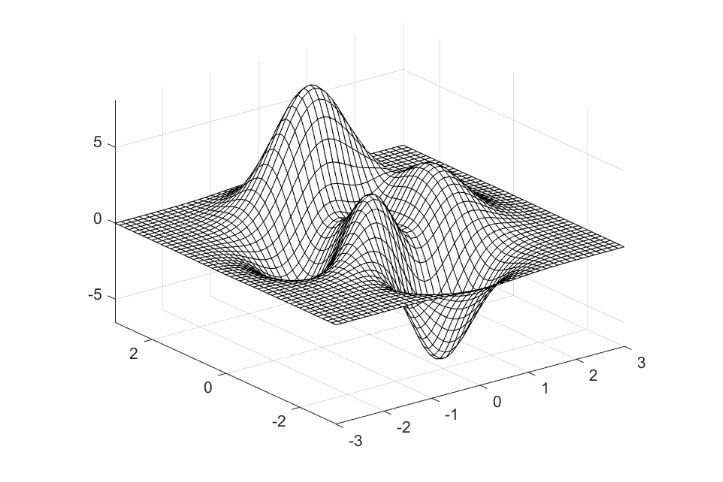
\includegraphics{matlab}

In parallel to MATLAB and R, Python represents the advent of the so-called scripting languages. Scripting languages are programming  languages which offer readability and versatility, along with decoupling from the actual operating system that it is being executed on. System languages, such as C, are designed and used in order to interact directly with the computer hardware, and to constitute data structures from the ground up\cite{ousterhout_scripting_1998}. On the other hand, scripting languages were designed and used in order to connect existing software systems or data sources together, most notably in the early days of shell scripting (such as \lstinline{Bash}, \lstinline{sed} or \lstinline{awk}). Starting with the late 1990s, and the appearance of languages such as Perl\footnote{First version developed in 1987 by Larry Wall} and Python\footnote{First official release in 1991 by Guido Van Rossum}, scripting languages became more widely used by non-programmers who already had data to work with and needed tools to exploit it. In the following decades, the development of additional scientific libraries such as \emph{SciKit}, \emph{NumPy} for mathematics and numerical work or \emph{NLTK} for language processing and social sciences in Python complemented the language's ease of use by providing manipulation of complex scientifc concepts\cite{millman_python_2011}, a phenomenon of user-extension which has also been observed in R and MATLAB's ecosystems\cite{moler_history_2020}.

This steady rise of scientific computing has nonetheless highlighted the apparent lack of quality standards in academic software, and how the lack of value judgments on the software written might impact the reliability of the scientific output. Perhaps the most well-known example of such a lack is the one revealed by the leak of the source code of the Climate Research Unit from the University of East Anglia in 2009\cite{merali_computational_2010}. In the leak, inline comments of the authors, as well as code reviews of external software developers point out to the CRU leak as being a symptom of the state of academic software. As Professor Darrel Ince stated to the UK Parliamentary Committee in February 2010:

\begin{quote}
There is enough evidence for us to regard a lot of scientific software with worry. For example Professor Les Hatton, an international expert in software testing resident in the Universities of Kent and Kingston, carried out an extensive analysis of several million lines of scientific code. He showed that the software had an unacceptably high level of detectable inconsistencies.\cite{committee_disclosure_2010}
\end{quote}

As a response to this realization, the beginning of the 2000s has seen the desire to re-integrate the best practices of software engineering in order to correct scientific software's lack of accuracy\cite{hatton_how_1994}. Indeed, software engineering, as we've seen above, had developed on their own since its establishment as an independent academic discipline and professional field. Such a split, described by Diane Kelly as a "\emph{chasm}"\cite{kelly_software_2007} then had to face the different standards to which commercial software and scientific software are subject to. For instance, commercial software must be extensible and performant, two qualities that do not necessarily translate to an academic setting, in which software might be written within a specific, time-constrained, research project, or in which access to computing resources (i.e. supercomputers) might be less of a problem.

Within Landau et. al's conception of the scientific process as the progression from problem to theory, followed by the establishment of a model, the devising of a method, and then on to implemementation and finally to assessment\cite{landau_survey_2011}, code written as academic software is now involved in the latter two stages of  method and implementation. Within those two stages, software has to abide by the processes and requirements of scientific research. First and foremost, reproducibility is a core requirement of scientific research in general\footnote{This requirement dates back the 1600s with Robert Boyle and the Invisible College in England\cite{leveque_reproducible_2012}} and bugs in a scientific software system can lead to radically different ouptuts given slightly different input data, while concealing the origin of this radical difference. Good academic code, then, is one which defends actively against these, perhaps to the expense of performance and maintainability. This can be addressed by reliable error-handling, regular assertions of the state of the processed data and extensive unit testing\cite{wilson_best_2014}.

Furthermore, a unique aspect of scientific software comes from the lack of clear upfront requirements. Such requirements, in software development, are usually provided ahead of the programming process, and should be as complete as possible. As the activity of scientists is defined by an incomplete understanding of the application domain, requirements tend to emerge as further knowledge is developed and acquired\cite{segal_when_2005}. As a result, efforts have been made to familiarize scientists with software development best practices, so that they can implement quality software by themselves. Along with field-specific textbook\footnote{See \emph{Effective Computation in Physics}\cite{scopatz_effective_2015} or \emph{A Primer for Computational Biology}\cite{oneil_primer_2019} as textbooks covering similar software-oriented material from different academic perspectives.} the most prominent initiative in the field is \emph{Software Carpentry}, a collection of self-learning and teaching resources which aims at implementing software best practices across academia, for scientists and by scientists. Founded by Greg Wilson, the co-editor of \emph{Beautiful Code}, the organization's title refers directly to equivalents in the field of software development\footnote{See 1.1.2 \emph{Features of the field} above fo a discussion of the literature on writing good code for software developers)}.

We conclude here on a convergence of quality standards of broad academic software towards the quality standards of commercial software development\footnote{See Graphbrain at \url{https://github.com/graphbrain/graphbrain} for such an example. The code's organization and formal features are congruent and on par with commercial software.}.  And yet, this convergence is due to, as we've seen, a past divergence between computation and science, as computer science worked towards asserting and pursuing its own field of research. As a subset of science, computer science nonetheless holds specific standards, taking software not as a means to an end, but as the end itself.

\vspace*{1\baselineskip}

\subsubsection{Computation as an end}


Computer scientists are scientists whose work focuses on computation as a means, rather than as a tool. As such, they study the phenomenon of computation, investigating its nature and effects through th development of a theoretical frameworks around it. Originally derived from computability theory, as a branch of formal mathematical logic, computation emerged as an autonomous field from work in mechanical design and configuration (Ada Lovelace and Charles Babbage),  work on circuit and language design (C. S. Pierce, Konrad Zuse and John Von Neumann), work on mathematical foundations (Alan Turing and Alonzo Church), information theory (Claude Shannon), systems theory (Norbert Wiener) and expert systems (John McCarthy and Marvin Minsky)\cite{ifrah_universal_2001}. In the middle of such a constellation ranging from mathematical theory to practical electronics, computer science establishes institutional grounding with the inauguration of the first dedicated academic deparment at Purdue University in 1962.

From this multifaceted heritage and academic interdisciplinarity, computer scientists have established the some of the foundations of the field, identifying key areas such as data structures, algorithms and language design as the foundations of the discipline\cite{wirth_algorithms_1976}. Through the process, the tracing of the "roots" of computation remained a constant debate as to whether computer science exists within the realm of mathematics, of engineering or as a part of the natural sciences. The logico-mathematical model of computer science contends that one can do computer science without a computer, solely armed of a pen and a paper, while the engineering approach of computer science tends to put more practical matters, such as architecture, language design and systems programming at the core of the discipline; both being a way to generate and process information as natural phenomenon\cite{tedre_development_2006}.

The broad difference we can see between these different conceptions of computer science is that of \emph{episteme} and \emph{techne}. On the theoretical and scientific side, computer science is concerned with the primacy of ideas, rather than of implementation. The quality of a given program is thus deduced from its formal (in the mathematical sense) properties, rather than its formal (in the aesthetic sense) properties. The first manifestations of such a theoretical focus can be found in the Information Processing Language (1956), which was designed and developed originally to prove Bertrand Russell's \emph{Principia Mathematica}. While the IPL, as one of the very first programming languages, influenced the development of multiple subsequent languages, not least of all being LISP, some later languages came to be known as logic programming languages, based on a formal logic syntax of facts, rules and clauses about a given domain and whose correctness can be easily proven (see \ref{prolog} below for an example of the \emph{Prolog} logic programming language).

\begin{lstlisting}[caption={Prolog sample source}, label={prolog}, float, floatplacement=H]
  % induce(E,H) <- H is inductive explanation of E
induce(E,H):-induce(E,[],H).

induce(true,H,H):-!.
induce((A,B),H0,H):-!,
	induce(A,H0,H1),
	induce(B,H1,H).
induce(A,H0,H):-
	/* not A=true, not A=(_,_) */
	clause(A,B),
	induce(B,H0,H).
induce(A,H0,H):-
	element((A:-B),H0),     % already assumed
	induce(B,H0,H).         % proceed with body of rule
induce(A,H0,[(A:-B)|H]):-       % A:-B can be added to H
	inducible((A:-B)),      % if it's inducible, and
	not element((A:-B),H0), % if it's not already there
	induce(B,H0,H).         % proceed with body of rule
\end{lstlisting}

Due to its Turing-completeness, one can write programs such as language processing, web applications, cryptography or database programming (using the \emph{Datalog} variant of \emph{Prolog}), but its use remains limited outside of theoretical circles in 2021\footnote{See the Stackoverflow Developer survey \url{https://insights.stackoverflow.com/survey/2021}}. Another programming language shares this feature of theoretical soundness faced with a limited range of actual use in production environments, Lisp—\emph{LISt Processor}—designed to process lists. It was developed in 1958, the year of the Dartmouth workshop, on Artificial Intelligence by its organizator, John McCarthy. Inheriting from IPL, it retained the core idea that programs should separate the knowledge of the problem (input data) and ways to solve it (internal rules), assuming  the rules are independent to a specific problem.

The base structural elements of LISP are not symbols, but lists (of symbols, of lists, of nothing), and they themselves act as symbols (e.g. the empty list). By manipulating those lists recursively—that it, processing something in terms of itself—Lisp highlights  even further this tendency to separate itself from the problem domain, and to exhibit autotelic tendencies. This is facilitated by its atomistic and relational structure: in order to solve what it has do, it evaluates each symbol and traverses a tree-structure in order to find a terminal symbol. Building on these features, Willam Byrd, computer scientst at the University of Utah, describes the following lines of Scheme (a LISP dialect) as "the most beautiful program ever written"\cite{byrd_william_2017}, a Scheme interpreter written in Scheme (\ref{scheme}):

\begin{lstlisting}[caption={Scheme interpreter written in Scheme}, label={scheme}, float, floatplacement=H]
  (define (eval-expr env)
  (lambda (expr env)
    pmatch expr
      [,x (guard (symbol? x))
        (env x)]
      [(lambda (,x) ,body)
        (lambda (arg)
          (eval-expr body (lambda (y)
                                          (if (eq? x y)
                                                arg
                                                (env y)))))]
        [(,rator ,rand)
          ((eval-expr rator env)
            (eval-expr rand env))]))
\end{lstlisting}

%include quote of nielsen: By making concrete what was formerly abstract, the code for our Lisp interpreter gives us a new way of understanding how Lisp works. https://michaelnielsen.org/ddi/lisp-as-the-maxwells-equations-of-software/

The beauty of such a program, for Byrd, is the abilty of these fourteen lines to reveal powerful and complex ideas about the nature and process of computation. As an interpreter, this program can take any valid Scheme input and evaluate it correctly. It does so by showing and using ideas of recursion (with calls to \lstinline{eval-expr}), environment (with the evaluation of the \lstinline{body}) and lambda functions, as used throughout the program. Following Alan Kay, creator of the Smalltalk programming language, Byrd equates the feelings he experiences in witnessing and pondering the program above to those suggested by Maxwell's equations, which constitute the foundation of classical electromagnetism (\ref{maxwell})\cite{kay_conversation_2004}. In both cases, then, the quality ascribed to those inscriptions come from the simplicity and conciseness of their base elements—making it easy to understand what the symbols mean and how we can compute relevant outputs—all the while implying complex consequences for both, respectively, computer science and electromagnetism.

\begin{equation}
  \begin{aligned}
  \frac{\partial\mathcal{D}}{\partial t} \quad & = \quad \nabla\times\mathcal{H}
  \frac{\partial\mathcal{B}}{\partial t} \quad & = \quad -\nabla\times\mathcal{E}
  \nabla\cdot\mathcal{B}                 \quad & = \quad 0 
  \nabla\cdot\mathcal{D}                 \quad & = \quad 0                       
  \end{aligned}
  \end{equation}

With this direct manipulation of symbolic units upon which logic operations can be executed, Lisp became the language of AI, an intelligence conceived first and foremost as abstractly logical, if not outright algebraic. Lisp-based AI was thus working on what Seymour Papert has called "toy problems"—self-referential theorems, children's stories, or simple puzzles or games. In these, the problem and the hardware are reduced from their complexity and multi-consequential relationships to a finite, discreete set of concepts and situations. Confronted to the real world—that is, to commercial exploitation—Lisp's model of symbol manipulation, which proved somewhat successful in those early academic scenarios, started to be applied to issues of natural language understanding and generation in broader applications. Despite disappointing reviews from government reports regarding the effectiveness of these AI techniques, commercial applications flourished, with companies such as Lisp Machines, Inc. and Symbolics offering Lisp-based development and support. Yet, in the 1980s, over-promising and under-delivering of Lisp-based AI applications, which often came from the combinatorial explosion deriving from the list- and tree-based representations, met a dead-end.

\vspace*{1\baselineskip}

"\emph{By making concrete what was formerly abstract, the code for our Lisp interpreter gives us a new way of understanding how Lisp works}", notes Michael Nielsen in his analysis of Lisp, pointing at how, across from the \emph{episteme} of computational truths stands the \emph{techne} of implementation\cite{nielsen_lisp_2012}. The alternative to such abstract, high-level language, is to consider computer science as an engineering discipline, a shift between theoretical programming and practical programming is Edsger Dijkstra's \emph{Notes on Structured Programming}. In it, he points out the limitation of considering programming only as a concrete, bottom-up activity, and the need to formalize it in order to conform to the standards of mathematical logical soundness. Djikstra argues for the superiority of formal methods through the need for a sound theoretical basis when writing software, at a time when the software industry is confronted with its first crisis\footnote{See section above.}.

Within the software engineering debates, the theory and practice vocabulary had slightly different tones, with terms like “art” and “science” labeling two different mindsets concerning programming\cite{knuth_art_1997}. As mentioned by Djikstra's example, software engineering suffered from an earlier image of programming as an inherently unmanageable, unsystematic, and artistic activity. There again, many saw programming essentially as an art or craft\cite{tedre_development_2006}, rather than an exact science. Beyond theoretical soundness, computer science engineering concerns itself with efficiency and sustainability, with measurements such as the \emph{O()} notation for program execution complexity. It's not so much about whether it is possible to express an algorithm in a programming language, but whether it is possible to run it effectively, in the contingent environments of hardware, humans and problem domains\footnote{Notably, algorithms in textbooks tend to be erroneous when used in production; only in five out of twenty are they correct\cite{pattis_textbook_1988}.}.

This approach, halfway between science and art, is perhaps best seen in Donald Knuth's magnum opus, \emph{The Art of Computer Programming}. In it, Knuth summarizes the findings and achievements of the field of computer science in terms of algorithm design and implementation, in order to "\emph{to organize and summarize what is known about the fast subject of computer methods and to give it firm mathematical and historical foundations.}"\cite{knuth_art_1997}. The art of computer programming, according to Knuth, is therefore based on mathematics, but nonetheless different from it insofar as it has to deal with effectiveness, implementation and contingency\footnote{\emph{The Art of Computer Programming} involves a hypothetical computer, called MIX, to implement the algorithms discussed.}. In so doing, Knuth takes on an empirical approach to programming, inspecting source code and running software to assess their performance, an approach he first inaugurated for FORTRAN programs when reporting on their concrete effectiveness for the United States Department of Defense\cite{defense_technical_information_center_dtic_1970}.

Another influential academic textbook dealing not just with computation as a an autotelic phenomenon is \emph{Structure and Interpretation of Computer Programs}, in which the authors insist that source code is "\emph{must be written for people to read, and only incidentally for machines to execute}"\cite{abelson_structure_1979}. Still, even when confronted with implementation and the plurality of contingencies of non-mathematical elements which accompany it, the aesthetic standard in this engineering approach to computer science is the proportionality between the number of lines of code written and the complexity of the idea explained, as we can see in the series \emph{Beautiful Julia Algorithms}\cite{moss_beautifulalgorithmsjl_2022}. For instance, \ref{bubble_sort} implements the Bubble Sort sorting algorithm in one loop rather than the usual two loops in C, but the simplicity of scientific algorithms is expressed even further in \ref{nearest_neighbor} the one-line implementation of a procedure for finding a given element's nearest neighbor, a crucial component of classification systems, including AI systems.

\begin{lstlisting}[caption={Bubble Sort implementation in Julia}, label={bubble_sort}, float, floatplacement=H]
function bubble_sort!(X)
for i in 1:length(X), j in 1:length(X)-i
    if X[j] > X[j+1]
        (X[j+1], X[j]) = (X[j], X[j+1])
    end
end
end
\end{lstlisting}

\begin{lstlisting}[caption={Nearest neighbor implementation in Julia}, label={nearest_neighbor}, float, floatplacement=H]
function nearest_neighbor(x', phi, D, dist)
  D[argmin([dist(phi(x), phi(x')) for (x,y) in D])][end]
end
\end{lstlisting}

According to Tedre, computer science itself was split in a struggle between correctness and productivity, between theory and implementation, and between formal provability and intuitive art. In the early developments of the field, when machine time was expensive and every instruction cycle counted, efficiency ruled over elegance, but in the end he assesses elegance prevailed, as we will see with the evolution of craft within programming in \hyperref[sec:craft]{section 1.4.1} below.

In closing, one should note that the \emph{Art} in the title of the book does not, however, refer to art as a fine art, or a purely aesthetic object. In a 1974 talk at the ACM, Knuth goes back to its Latin roots, where we find \emph{ars}, \emph{artis} meaning "skill.", noting that the equivalent in Greek being τεχνη, the root of both "technology" and "technique.". This semantic proximity helps him reconcile computation as both a science and an art, the first due to its roots in mathematics and logic, and the second

\begin{quote}
  because it applies accumulated knowledge to the world, because it requires skill and ingenuity, and especially because it produces objects of beauty. A programmer who subconsciously views himself as an artist will enjoy what he does and will do it better. Therefore we can be glad that people who lecture at computer conferences speak about the state of the Art.\cite{knuth_computer_1974}
\end{quote}

\vspace*{1\baselineskip}

When written within an academic and scientific context, we can see how source code tends to align with the aesthetic standards of software development, valuing clarity, reabability, sustainability, in particular through Greg Wilson's work on the development of software development principles through the Software Carpentry and Data Carpentry initiatives. This alignment can also be seen in a conception of computer science as a kind of engineering, as an empirical practice which can and should be formalized in order to become more efficient. There, one can turn to Donald Knuth's \emph{Art of Computer Programming} to see the connections between the academia's best practices and the industry's best practices. And yet, a practical conception of computation as engineering isn't the only conception of computer science. Within a consideration of computer science as a  theoretical and abstract object of study, source code becomes a means of providing insights into more complex abstract concepts, such as the Lisp interpreter, or one-line algorithms implementing foundational algorithms in computer science. It is this relation to a conception of beauty traditionally associated with mathematics and physics which we will investigate below. But first, we complete our overview of code practicionners by turning to the software artists. 

\pagebreak

\subsection{Poets - 2000}

\begin{itemize}
    \item history of creative coding
    \item digital art vs. software art
    \item code poets
\end{itemize}

\section{Ideals of beauty - 5000}

\subsection{Introduction to the Methodology - 1000}

Kintsch and Van Dijk

\subsection{Lexical Field in Programmer Discourse -4000}

Positive words (13p)

% dope case study https://queue.acm.org/detail.cfm?id=1039535 also this http://denninginstitute.com/pjd/GP/gp_summary_toplevel.html

\begin{itemize}
    \item clean
    \item simple
    \item elegant
    \item transparent/self-explanatory
\end{itemize}

Negative words (2p)

\begin{itemize}
    \item smelly
    \item entangled
\end{itemize}

\section{Types of beauty  - 20p}

Now that we've done some empirical work, we can try to abstract away a bit and then look into how this relates to existing frameworks of aesthetics. 

Now that \emph{we look at proofs, through discourse}, what kind of beauty can we be dealing with?

\subsection{Literary Beauty}

This second approach contrasts with the functional component of the first one, but nonetheless stands in relationship with it. the creative beauty, by defying traditional beauty standards, does help us highlight, through deviance, what the norm is. These texts on "creative beauty" include the classical perl poetry, code poems, IOCC, code poetry contest, etc.

\subsection{Mathematical beauty}

Mostly elegance, could be a good place to work on the distinction between proof and theorem, concept and appearance.

\subsection{Architectural beauty}

This allows a segue into everyday aesthetics and environmental aesthetics

\section{Craft and beauty - 10p}
\label{sec:craft}

Now that we've seen how the aesthetic ideals of code borrow from different registers, we need to think about practice, or ways. all of the above can be seen through the prism of craft

\subsection{Functional beauty}

This first approach, by comparing both source and comment at the same time (taking texts which are explicitly described as being beautiful), explicitly highlights the requirements for source code to be beautiful. 

There is also an emerging development in aesthetics of integrating function as a criteria for an aesthetic experience.

\subsection{Embodiment}

also note the place and role of tools (IDEs, teletypes, fast compiling, etc.)

\subsection{Tacit knowledge}

%or at least the role of knowledge, mind as matter:https://dl.acm.org/doi/10.1007/s11023-007-9060-8

\pagebreak

\chapter{Understanding source code}

Aesthetics in source code are thus primarily related to cognitive load. In the previous chapter, we've highlighted a focus on understanding when it comes to aesthetic standards: whether obfuscating or illuminating, the process of acquiring a mental model of a given object is a key determinant in the value judgment as applied to source code. In this chapter, we focus on the reason for which such a cognitive load exists in the first place, before surveying the means—both linguistic and mechanistic—that programmers deploy in order to relieve such a load.

This is related to one of the essential features of software: it must be \emph{functional}. As mentioned in our discussion of the differences between source code and software in the introduction, source code is the latent description of what the software will ultimately \emph{do}. Similarly to sheet music, or to cooking recipes\footnote{Recipes are a recurring example taken to communicate the concept of an algorithm to non-experts \citep{zeller_algorithms_2020}}, they require to be put into action in order for their users (musicians and cooks, respectively) to assess their value. Therefore, buggy or dysfunctional software is going to be of less value than correct software \citep{hill_what_2016}, regardless of how aesthetically pleasing the source is.

The assessment of whether a piece of software functions correctly is essentially an assessment of whether what the software does is what the software is supposed to do, which in turn entails knowing what it does, what it is supposed to do, and being able to tell whether these two things are aligned. Any value judgment regarding the aesthetics of the source code at hand would be subject to whether or not the software functions correctly, and such judgment is rendered moot if that software does not work.

After deciding on a benchmark to assess the functionality of the source code at hand (understanding what it should be doing), one must then determine the actual behavior of the source code at hand once it is executed (understanding what it is actually doing). This chapter examines what goes into understanding source code. The first part will lay out our definition of understanding, presenting it as a dual phenomenon, between formalism and contextualism. Starting with 20\^{th} century epistemology, we will see that a dominantly rational, cognitivist perspective on the nature of understanding, as it has been hailed by theoretical computer science research, shows its limits when confronted with practice. Having highlighted this tension, we then turn to how understanding the phenomenon of computation specifically, both on an ontological level, and on a psychological level. The ontological approach will show some of the features of software give it the status on an "abstract artifact", making it a complex object to grasp; the psychological approach will show how such a comprehension takes place for a varity of programmers. Finally, we will conclude with the means that programmers deploy to grasp the concepts at play with software: starting from metaphors used by the general public, we will go down this ladder of abstraction in order to reach the technical apparatuses used in the development and inspection of source code.

The main questions that this chapter addresses are the following: given a certain nature of knowledge acquisition, what are some of the features of computers that make them hard to grasp, and what kind of techniques are deployed in order to address these hurdles and in order to understand what the code is actually doing. This will have us investigate the relationship of knowing and doing, the nature of computation (what is software?) and its relationship to the world as it appears to us (how does modelling and abstraction translate a problem domain into software?), and the cognitive scaffoldings set up to facilitate that task.

% first the definition of understanding
\section{Formal and contextual understandings} %22k char

This section focuses on our definition of understanding—the process of acquiring a working knowledge of an object. Such definition relies on two main aspects: a formal, abstract understanding, and a more subjective, empirical one. We will see how the former had some traction in computer sciences circles, while the second gained traction in programming circles. To support those two approaches, we first trace back the genealogy of understanding in theoretical computer science, before outlining how concrete experience and situatedness outline an alternative tradition.

\subsection{Between formal and informal} %10k

\subsubsection{Theoretical foundations of formal understanding}

To start this inquiry, we go back to the early 20\^{th} century in Cambridge, when the theoretical roots of modern computation were being laid by both philosophers of logic and mathematicians, such as Bertand Russell, Ludwig Wittgenstein, and Alan Turing, as they worked on the formalization of thinking.

Wittgenstein, in particular, bases his argumentation in his \emph{Tractatus Logico-philosophicus} on the fact that much of the problems in philosophy are rather problems of understanding between philosophers—if one were to express oneself clearly, and to articulate one's through clear, unambiguous language, a common conclusion could be reached without much effort:

\begin{quote}
    Most questions and propositions of the philosophers result from the fact that we do not understand the logic of our language. \citep{wittgenstein_tractatus_2010}
\end{quote}

Language and logic are, as we see here, closely connected. Articulated in separate points and sub-points, his work conjugates aphorisms with logical propositions depending on one another, developing from broader statements into more specific precisions. Wittgenstein hints at the intertwining of language as a form of logic, and as logic as a form of language. In this, he follows in the footsteps of Gottfried Leibniz's \emph{Ars Combinatoria}, insofar Leibniz views reasoning and inter-subjective understanding as a formal problem. A universal, and universally-understandable language, called a \emph{characteristica universalis} could resolve any misunderstanding issues. Quoted by Russell, Leibniz notes that:

\begin{quote}
    If we had it [a characteristica universalis], we should be able to reason in metaphysics and morals in much the same way as in geometry and analysis... If controversies were to arise, there would be no more need of disputation between two philosophers than between two accountants [...] Let us calculate. \citep{russell_logical_1950}
\end{quote}

Centuries after Leibniz's declaration, Wittgenstein presents a coherent, articulated theory of meaning through the use of mathematical philosophy, and logic, and his work fits with that of Russell\footnote{In his \emph{Principia Mathematica}, he lays out a theory of logical expression} and Frege\footnote{The \emph{Begriffschrift} similarly attempts to constitute a language in which all scientific statements could be evaluated \citep{korte_frege_2010}, while \emph{Über Sinn und Bedeutung} clarifies the semantic uncertainties between a specific sentence and how it means, or refers to a concept}; even though these are different theories, they are part of a similar endeavour to find a basis od formal propositions through which one could establish truth-values. Such attempt was a direct influence in the work on mathematician Alan Turing—who studied at Cambridge and followed some of Wittgenstein's lectures—, as he developed his own formal system for solving complex, abstract mathematical problems, manifested as a symbolic machine \citep{turing_computable_1936}.

The design of the Turing machine is a subsequent step engagement with the question of understanding in the philosophical sense, as well as in the practical sense—a formal proof to the \emph{Entscheidungsproblem} solved mechanically. Indeed, it is a response to the questions of translation (of a problem) and of implementation (of a solution). This formal approach to instructing machines to operate on logic statements then prompted Turing to investigate the question of intelligence and comprehension in \emph{Computing Machinery and Intelligence}. In it, he translates the hazy term of "thinking" machines into that of "conversing" machines, conversation being a practical human activity which involves listening, understanding and answering (i.e. input, process and output) \citep{turing_computing_2009}. This conversational test, which has become a benchmark for machine intelligence, does rely on the need for a machine to \emph{understand} what is being said. Throughout the article, however, Turing does not yet address the need for a purely formal approach of whether or not a problem can be translated, as Leibniz would have it, into atomistic symbols which would be provided as an input to a digital computer. Such a process of translation would rely on a formal approach, similar to that laid out in the \emph{Tractatus Logico-philosophicus}, or on Frege's formal language described in the \emph{Begriffschrift}. Following a cartesian approach, the idea in both authors is to break down a concept, or a proposition, into sub-propositions, in order to recursively\footnote{although it was not called as such at the time} establish the truth of each of these sub-propositions, and then re-assembled to deduce the truth-value of the original proposition. While Turing focuses on the philosophical and moral arguments to the possibility for machines to think, he does address the issue of artificial intelligence.

With these sophisticated syntactic systems developed a certain approach to cognition, as Turing clearly establishes parallels between the digital computer and the human brain. We now turn to the form of these systems, looking at how their form addresses the problem of clearly understanding and operating on mathematical and logical statements.

Logical calculus, as the integration of the symbol into relationships of many symbols formally takes place through two stylistic mechanisms, the \emph{symbol} and the \emph{list}. Each of the works by Frege, Russell and Wittgenstein quoted above are structured in terms of lists and sub-lists, representing the stylistic pendant to the epistemological approach of related, atomistic propositions and sub-propositions. A list, far from being an innate way of organizing information in humans, is a particular approach to language: extracting elements from their original, situated existence, and reconnecting ways in very rigorous, strictly-defined ways. As Jack Goody writes in \emph{The Domestication of the Savage Mind},

\begin{quote}
    [List-making] [...] is an example of the kind of decontextualization that writing promotes, and one that gives the mind a special kind of lever on 'reality'. \citep{goody_domestication_1977}
\end{quote}

As inventories, early textbooks, administrative documents as public mnemotechnique, the list is a way of taking symbols, pictorial language elements in order to re-assemble them to reconstitute the world, then re-assemble it from blocks, following an assumption that the world can always be decomposed into smaller, discreete and \emph{conceptually coherent} units (i.e. symbols). The list, Goody continues, establishes clear-cut boundaries, they are simple, they are abstract and discontinuous.

Being based on some singular, symbolical entity, applying logical calculus to lists and their symbols, and doing so in a computing environment, becomes the next step in exploring these tools for thinking. Indeed, the engineering development of digital computers in post-war United States as described in \ref{subsec:software-developers}, allowed for the putting into practice of these languages, in the budding field of artificial intelligence (AI).

\subsubsection{Practical attempts at implementing formal understanding}

This putting into practice took the form of subsequent programming languages, relying on a certain conception of human cognition—abstract, logical, as shown above.

IPL, the Information Processing Language, was created by Allen Newell, Cliff Shaw and Herbert A. Simon.  The idea was to make programs understand and solve problems, through "the simulation of cognitive processes" \citep{newell_information_1964}. IPL achieves this with the symbol as its fundamental construct, which at the time was still largely mapped to physical addresses and cells in the computer's memory, and not yet decoupled from hardware.

% add example of IPL
A link between the ideas exposed in the writing of the mathematical logicians and the actual design and construction of electrical machines activating these ideas, IPL was originally designed to demonstrate the theorems of Russell's \emph{Principia Mathematica}, along with a couple of early AI programs, such as the \emph{Logic Theorist}, the \emph{General Problem Solver}. More a proof of concept than a versatile language, IPL was then quickly replaced by LISP as the linguistic means to express intelligence in digital computers.

% add figure on what lisp looks like
LISP (\emph{LIst Processor}) was developed in 1956 was Joseph McCarthy\footnote{McCarthy coined the phrase \emph{Artificial Intelligence} during the 1956 Dartmouth workshop}. The base structural elements of LISP are not symbols, but lists (of symbols, of lists, of nothing), and they themselves act as symbols (e.g. the empty list) \citep{mccarthy_history_1978}. By manipulating those lists recursively—that it, processing something in terms of itself—Lisp shows a tendency for a formal system to separate itself from the problem domain. This is facilitated by its atomistic and relational structure: in order to solve what it has do, it evaluates each symbol and traverses a tree-structure in order to find a terminal symbol, without the explicit need to refer to an external table, for instance.

% add figure on tree structure of language
This sort of heuristic is quite similar to the approach suggested by Noam Chomsky in his \emph{Syntactic Structures}, where he posits the tree structure of language, as a decomposition of sentences until the smallest conceptually coherent parts (e.g. Phrase -> Noun-Phrase + Verb-Phrase -> Article + Substantive + Verb-Phrase). The style is similar, insofar as it proposes a general ruleset (or the at least the existence of one) in order to construct complex structures through simple parts.

Through its direct manipulation of conceptual units upon which logic operations can be executed, LISP became the language of AI, an intelligence conceived first and foremost as logical understanding. The use of LISP as a research tool culminated in the \emph{SHRDLU} program, a natural language understanding program built in 1968-1970 by Terry Winograd which aimed at tackling the issue of situatedness—AI can understand things abtractly through logical mathematics, but can it apply these rules within a given context? The program had the particularity of functioning with a "blocks world" a highly simplified version of a physical environment—bringing the primary qualities of abstraction into solid grasp. The computer system was expected to take into account the rest of the world and interact in natural language with a human, about this world (\emph{Where is the red cube?} \emph{Pick up the blue ball}, etc.). While incredibly impressive at the time, \emph{SHDRLU}'s success was nonetheless relative. It could only succeed at giving barely acceptable results within highly symbolic environments, devoid of any noise. In 2004, Terry Winograd writes:

\begin{quote}
    There are fundamental gulfs between the way that SHRDLU and its kin operate, and whatever it is that goes on in our brains. I don’t think that current research has made much progress in crossing that gulf, and the relevant science may take decades or more to get to the point where the initial ambitions become realistic.  \citep{nilsson_quest_2009}
\end{quote}

This attempt, since the beginning of the century, to enable thinking, clarify understanding and implement it in machines, had first hit an obstacle. The world, also known as the problem domain, exhibits a certain complexity which did not seem to be easily translated into singular, atomistic symbols. Around the same time, however, was developed another approach to formalizing the intricacies of cognition.

Warren McCullough's seminal paper, \emph{A logical calculus of the ideas immanent in nervous activity}, co-written with Walter Pitts, offers an alternative based on the embodiment of cognition. They present a connection between the systematic, input-output procedures dear to cybernetics with the predicate logic writing style of Russell and others \citep{mcculloch_logical_1990}. This attachment to input and output, to their existence in complex, inter-related ways, rather than self-contained propositions is, interestingly, rooted in his activy as a literary critic\footnote{Even at the Chicago Literary book club, he argues for a more sensuous approach to cognition: \emph{"In the world of physics, if we are to have any knowledge of that world, there must be nervous impulses in our heads which happen only if the worlds excites our eyes, ears, nose or skin."} \citep{mcculloch_delusion_1953}}.

Going further in the processes of the brain, he indeed finds out, in another paper with Letvinn and Pitts \citep{lettvin_what_1959}, that the organs through which the world excites the brain \emph{are themselves} agents of process, activating a series of probabilistic techniques, such as noise reduction and softmax, to provide a signal to the brain which isn't the untouched, unary, \emph{symbolical} version of the signal input by the external stimuli, and nor does it seem to turn it into such.

We see here the development of a theory for a situated, embodied stance towards cognition, which would ultimately resurface through the rise of machine learning via convoluted neural networks in the 2000s \citep{nilsson_quest_2009}. In it, the senses are as essential as the brain for an understanding—that is, for the acquisition, through translation, of a conceptual model which then enable deliberate and successful action. It seems, then, that there are other ways to know things than to rely on description through formal propositions.

\vspace*{1\baselineskip}

A couple of decades later, Abelson and Sussman still note, in their introductory textbook to computer science, the difficulty to convey meaning mechanically:

\begin{quote}
    Understanding internal definitions well enough to be sure a program means what we intend it to mean requires a more elaborate model of the evaluation process than we have presented in this chapter. \citep{abelson_structure_1979}
\end{quote}

While formal notation is able to enable digital computation, it nonetheless proved to be limited when it came to accurately and expressively  conveying meaning. This limitation, of being able to express formally what we understand intuitively (e.g. \emph{what is a chair?}\footnote{A question addressed by Joseph Kosuth in his artwork \emph{One and Three Chairs}, 1965}) appeared as computers applications left the domain of logic and arithmetic, and were applied to more social domains.

After having seen the possibilities and limitations of making machines understand through the use of formal languages, and the shift offered by taking into account sensory perception as a possible locus of cognitive processes, we now turn to these ways of knowing that exist in humans in a more embodied capacity.

% todo
% \begin{itemize}
% \item EXAMPLE: XML (applen, mcdaniel, rhetorics of xml)
% \end{itemize}

\subsection{Knowing-what and knowing-how} %10k

1953 saw a radical posture change from one of the logicians whose work underpinned AI research, briefly before the start of these attempts to implement artificial intelligence in digital computers. This was the publication of Wittgenstein's \emph{Philosophical Investigations}. In his second work, he disown his previous approach to language as seen in the \emph{Tractatus Logico-philosophicus}, and favors a more contextual, use-centered frame. Rather than what knowledge is, he looks at how knowledge is acquired and used; while (formal) lanuage was previously defined as the exclusive means to translation concepts in clearly understandable terms, he broadens his perspective in the \emph{Inquiries} by stating that language is \emph{"the totality of language and the activities with which it is intertwined"} and that \emph{"the meaning of a word is its use within language"} \citep{wittgenstein_recherches_2004}, noting context and situatedness as a important factors in the understanding process.

At first, then, it seemed possible to make machines understand through the use of formal languages. The end of the first wave of AI development, as a branch of computation specifically focused on cognition, have shown some limits to this approach.  We now turn to theories which support this approach of an embodied and contextualized knowing, complemented by a constructivist approach to building an understanding.

% 4000
\subsubsection{Knoweldge and situation}

As hinted at by the studies of McCullough and Levitt, understanding a situation doesn't rely exclusively on abstract logical processes, but also on the processes involved in grasping this situation, such as, in their case, peripheral vision processing. It is not just what things are, but how they are, and how they are \emph{perceived}, which matters. Different means of inscription and description do tend to have an impact on the ideas communicated and understood.

In his book \emph{Making Sense: Cognition, Computing, Art and Embodiment}, Simon Penny refutes the so-called unversality of formulating cognition as a formal problem, and develops an alternative history of cognition, akin to Michel Foucault's archeology of knowledge. Drawing on the works of authors such as William James, Jakob von Uexküll and Gilbert Ryle, he refutes the Cartesian dualism thesis which acts as the foundation of AI research \citep{penny_making_2019}. A particular example of the fallacy of dualism, is the use of the phrase \emph{implementation details}, which he recurringly finds in the AI literature, such as Herbert Simon's \emph{The Sciences of the Artificial} \citep{simon_sciences_1996}. The phrase refers to the gap existing between the statement of an idea, of an algorithm, and a procedure, and its concrete, effective and functional manifestation.

For instance, pseudo-code is a way to sketch out an algorithmic procedure, which might be considered agnostic when it comes to implementation details. One can consider the pseudo-code in \ref{code:nielsen_chalktalk}, which describes a procedure to recognize a free-hand drawing and transform it into a known, formalized glyph. Disregarding the implementation details means disregarding any reality of an actual system: the operating system (e.g. UNIX or MSDOS), the input mechanism (e.g. mouse, joystick, touch or stylus), the rendering procedure (e.g. raster or vector), or the programming language (e.g. JavaScript or Python).

\begin{listing}
    \begin{minted}{python}
        recognition = false
        do until recognition
        wait until mousedown
            if no bounding box, initialize bounding box
            do until mouseup
            update image
            update bounding box
            rescale the material that's been added inside
            if we recognize the material:
                delete image from canvas
                add the appropriate iconic representation
                recognition = true
    \end{minted}
    \caption[]{Example of pseudo-code attempting to reverse-engineer a software system, ignoring any of the actual implementation details, taken from \citep{nielsen_working_2017}}
    \label{code:nielsen_chalktalk}
\end{listing}

Refuting the idea that pseudo-code is all that is necessary to communicate and act upon a concept, Penny  argues on the contrary that information is relativistic and relational; relative to other pieces of information (intra-relation) and related to contents and forms of presenting this relation (extra-relation). Pseudo-code will only ever make sense in a particular implementation context, which then affects the product.

He then follows Philip Agre's statement that a theory of cognition based on formal reason works only with objects of cognition whose attributes and relationships can be completely characterized in formal terms; and yet a formalist approach to cognition does not prove that such objects exist or, if they exist, that they can be useful. Uses of formal systems in artificial intelligence in specific, and in cognitive matters in general, is yet another instance of the map and the territory problem—it only goes so far.

Beyond the syntax of formal logic, there are different ways to transmit cognition in actionable form, depending on the form, the audience and the purpose. In terms of form, a symbol system of formal logic is only one of many possibilities for systems of forms. In his \emph{Languages of Art}, Nelson Goodman elaborates a theory of symbol systems, which he defines as formal languages composed of syntactic and semantic rules \citep{goodman_languages_1976}. Logical notation exists along with music, painting, poetry and prose. What follows, argues Goodman, is that all these formal languages involve an act of \emph{reference}. Through different means (exemplification, denotation, resemblance, representation), formal systems act as sets of symbols which can denote or exemplify or refer to in more complex and indirect ways, yet always between a sender and a receiver\footnote{Understood as the eponymous entities  in Jakobsen's model of communication functions.}.

Communication, as the transfer of meaning from one individual to one or more other individuals, does not exclusively rely on the use of mathematical based use of formal languages. From Goodman to Goody, the format of representation also affords differences in what can be thought and imagined. Something that was always implicit in the arts—that representation is a complex and ever-fleeting topic—is shown more recently in Marchand-Zañartu and Lauxerois's work on pictural representations made by philosophers, visual artists and novelists (such as Claude Simon's sketches for the structure of his novel \emph{La Route des Flandres}, shown in \ref{image:routedesflandres}) \citep{marchand-zanartu_32_2022}. How specific domains, from mathematics to visual arts and construction, engage in the relation between form and cognition is further adressed in CHAPTER\_4.

\begin{figure}
    \begin{center}
        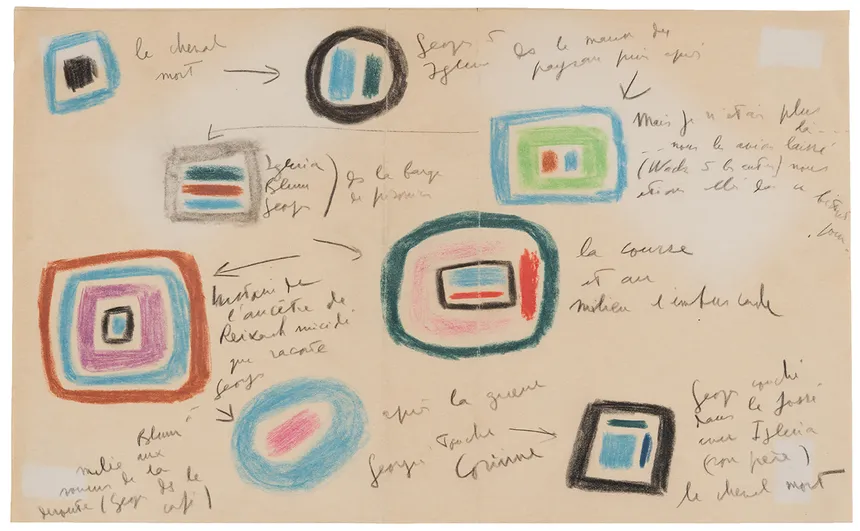
\includegraphics[width=\textwidth,height=\textheight,keepaspectratio]{routedesflandres.png}
        \caption{Tentative d'organisation visuelle pour le roman La Route des Flandres, années 1960 - Claude Simon, écrivain}
        \label{image:routedesflandres}
    \end{center}
\end{figure}

Going beyond logical notation, we have seen that there are other conceptions of knowledge which take into account the physical, social and linguistic context of an action. Nonetheless, these can still be systematized, as Goodman highlights in his investagation of referential systems, with a focus on reference of the ideas at hand.

% 4000
\subsubsection{Constructing knowledge}

There are multiple ways to express an idea: on can use formal notation or draft a rough sketch with different colors. These all highlight different degrees of expression, but one particular way can be considered problematic in its ambition. Formal languages rely on the assumption, that all which can be known can ultimately be expressed in unambiguous terms. First shown by Wittgenstein in the two main eras various eras of his work, we know focus on the ways of knowing which cannot be explicited.

First of all, there is a separation between \emph{knowing-how} and \emph{knowing-that}; the latter, propositional knowledge, does not cover the former, practical knowledge, as shown by Ryle \citep{ryle_concept_1951}. Perhaps one of the most obvious example of this duality is in the failure of Leibniz to construct a calculating machine, as told by Matthew L. Jones in his book \emph{Reckoning with Matter}. In it, he traces the history of philosophers to solve the problem of constructing a calculating machine, a problem which would ultimately be solved by Charles Babbage, with the consequences that we know \citep{jones_reckoning_2016}.

Jones depicts Leibniz in his written correspondence with watchmaker Ollivier, in their fruitless attempt to construct Leibniz's design; the implementations details seem to elude the German philosopher as he refers to the "confused" knowledge of the nonetheless highly-skilled Parisian watchmaker. The (theoretical) plans of Leibniz do not match the (concrete) plans of Ollivier.

These are two complementary approaches to the knoweldge of something: to know \emph{what} constructing calculating machine entails and knowing \emph{how} to construct such a machne. In the fact that Ollivier could not communicate clearly to Leibniz what his technical difficulties, we can see an instance of something which would be theorized centuries later by Michael Polanyi as \emph{tacit knowledge}, knowledge which cannot be entirely made explicit.

Polanyi, as a scientist himself, starts from another assumption: we know more than we can tell. In his eponymous work, he argues against a positivist approach to knowledge, in which empirical and factual deductions are sufficient to achieve satisfying epistemological work. What he proposes, derived from \emph{gestalt} psychology, is to consider some knowledge of an object as the knowledge of an integrated set of particulars, of which we already know some features, by virtue of the object existing in an external approach. This integrated set, in turn, displays more properties than the sum of its parts. While formal notation suggests that the combination of formal symbols does not result in additional knowledge, Polanyi rather argues, against Descartes, that relations and perceptions do result in additional knowledge.

\begin{quote}
    The knowledge of a problem is, therefore, like the knowing of unspecifiables, a knowing of more than you can tell. \citep{polanyi_knowing_1969}
\end{quote}

Rooted in psychology, and therefore in the assumption of the embodimed of the human mind, Polanyi posits that all thought is incarnate, that it lives by the body and by the favour of society, hence giving it a physio-social dimension. This confrontation with the real-world, rather than being a strict hurdle that has to be avoided or overcome, as in the case of SHRDLU above, becomes one of the two poles of cognitive action. Knowledge finds its roots and evaluation in concrete situations, as much as in abstract thinking. In the words of Cecil Wright Mills, writing about his practice as a social scientist research,

\begin{quote}
    Thinking is a continuous struggle between conceptual order and empirical comprehensiveness. \citep{MillsC.WrightCharlesWright2000Tsi}
\end{quote}

Polanyi's presentation of a form of knowledge following the movement of a pendulum, between dismemberment and integration of concepts finds an echo in the sociological work of Mills: a knowledge of some objects in the world happens not exclusively through formal descriptions in logical symbol systems, but involves imagination and phenomenological experience—wondering and seeing. This reliance on vision—starting by recognizing shapes, as Polanyi states—directly implies the notion of aesthetic assessment, such as a judgement of typical or non-typical shapes. He does not, however, immediately elucidate how aesthetics support the formation of mental models at the basis of understanding, only that this morphology is at the basis of higher order of represenations.

Seeing, though, is not passive seeing, simply noticing. It is an active engagement with what is being seen. Mills's quote above also contains this other aspect of Polanyi's investigation of knowledge, and already present in Ollivier's relation with Leibniz: knowing through doing.

This approach has been touched upon from a practical programmer's perspective in section \ref{subsec:craft-knowledge}, through a historical lens but it does also posses theoretical grounding. Specifically, Harry Collins offers a deconstruction of the Polanyi's notion by breaking it down into \emph{relational}, \emph{somatic} and \emph{collective} tacit knowledges \citep{collins_tacit_2010}. While he lays out a strong approach to tacitness of knowledge (i.e. it cannot be communicated at all), his distinction between relational and somatic is useful here\footnote{His definition of collective tacit knowledge touches on the knowledge present in any living species and is impossible to ever be explicited, and is therefore out of scope here.}. It is possible to think about knowledge as a social construct, acquired through social relations: learning the linguo of a particular technical domain, exchanging with peers at conferences, imitating an expert or explaining to a novice. Collective, unspoken agreements and implicit statements of folk wisdom, or implicit demonstrations of expert action are all means of communication through which knowledge gets replicated across subjects.

Concurrently, somatic tacit knowledge tackles the physiological perspective as already pointed out by Polanyi. Rather than knowledge that exists in one's interactions with others, somatic tacit knowledge exists within one's physical perceptions and actions. For instance, one might base one's typing of one's password strictly on one's muscle memory, without thinking about the actual letters being typed, through repetition of the task. Or one might be spotting a cache bug which simply requires a machine reboot, due to experience machine lifecycles, package updates, networking behaviour. Not completely distinct from its relational pendant, somatic knowledge is acquired through experience, repetition and mimeomorphism—replicating actions and behaviours, or the instructions, often under the guidance of someone more experienced.

\vspace*{1\baselineskip}
\centerline{\rule{0.13334\linewidth}{.4pt}}
\vspace*{1\baselineskip}

We started our discussion of understanding by defining it as the acquisition of the knowledge of a object—be it a concept, a situation, an individual or an artfefact,, which is accurate enough that it allows us to predict the behaviour and to interact with such object. Within this defintion, one could take the example of a human discussion as a demonstration of advanced understanding, as something that is both situated, and formalized.

Theories of how individuals acquire understanding (how they come to know things, and know conceptual representations of things), have been approached from an explicit perspective, and an implicit one. In the rationalist, logical philosophical tradition, we have seen that the belief that meaning can be rendered unambiguous through the use of specific notation. This has led to the development of logic and computer science, as this meaning got mechanized. Explicit understanding is therefore the theoretical lineage of computation.

However, as we've seen in the first hurdles of artificial intelligence research, explicit specification of meaning falls short of handling everyday tasks which humans would consider to be menial. This has led us to consider a more implicit approach to understanding, in which it is acquired by tacit means. Particularly, we've identified this tacit knowledge as relying on a social component, as well as on a somatic component.

Source code, as a formal system with a high dependence of context, intent and implementation, mobilizes both approaches to understanding. Before we dive deeper about how these two modes of understanding are mobilized at the end of this chapter, we now turn to what makes computation a cognitively complex object, and what are some cognitive reactions that humans display in situations where they have to understand, and work with, software.

\clearpage

\section{Understanding computation}

In the previous chapter, we've laid out the groundwork by showing that there are multiple ways to understand something. We now turn to the thing we want to understand. What makes it challenging to understand computation?

First, we will inquire into some distinguishing features of software in terms of levels of abstractions, and in terms of types of complexity. This will highlight some of the theoretical properties that make it hard to understand, such as its relation to hardware, its relation to a specification, and its relation to time and space.

Then, we will shift our perspective to a more abstract point of view, investigating the ontological status of software. This will highlight how software exists as an \emph{abstract artifact}, simultaneously on the ideal, practical and physical plane.

Finally, we will conclude this section by looking specifically at the source code component of software, and how programmers deploy strategies to understand it. Approaching it from a cognitive and psychological perspective, this will give us a better picture of the concrete process of understanding source code—a process which aesthetics are primarily intended to affect.

% the software effect (combination of knowing what (it does) and how (it does it))
\subsection{Software complexity} %7k

Software exhibits several particularities, which result in a compex whole—meaning that software possesses several independent components which interact with each other in non-trivial, and non-obvious ways. This subsection focuses on these particularies; that is, on the \emph{properties} of software, and hence how these properties manifest themselves concretely, leading to those complex interactions. We will start by looking at the different levels at which software exists, before turning to the different kinds of complexity which make software hard to grasp.

\subsubsection{Levels of software} % 3k

One of the essential aspects of software is that of \emph{implementation}. Implementation is the realization of a plan, the concrete manifestation of an idea, and therefore hints at a first tension in software's multiple facets. It can happen through individuation, instantation, exemplification and reduction \citep{rapaport_philosophy_2005}. On the one side, there is what we will call here \emph{ideal} software, often existing only as a shared mental representation by humans (not limited to programmers), or as printed documentation, as a series of specifications, etc. On the other side, we have \emph{actual} software, which is manifested into lines of code, written in one or more particular languages, and running with more or less bugs.

The relationship between the \emph{ideal} and the \emph{actual} versions of the same software is not straightforward. Ideal software only provides an intent, a guidance towards a goal, assuming, but not guaranteeing, that this goal will be reached. A popular engineering saying is that complements this approach by stating that:

\begin{quote}
    In theory, there is no difference between theory and practice. In practice, there is.\footnote{Sometimes mis-attributed to Richard P. Feynman or Albert Einstein, but traced to Benjamin Brewster, writing in the Yale Literary Magazine of 1882.}
\end{quote}

Actual software, as most programmers know, differs greatly from its ideal version, largely due to the process of implementation, translating the purpose of the software from natural and diagrammatic languages, into programming languages, from what it should do, into what it actually does.

Writing on the myths of computer science, James Moor \citep{moor_three_1978} allows us to think through this distinction between ideal and practical along the lines of the separation between a theory and a model. The difference between a model and a theory is that both can exist independently of one another—one can have a theory for a system without being able to model it, while one can also model a system using \emph{ad hoc} programming techniques, instead of a coherent theory.

Most of the practice of programmers (writing and reading code for the purposes of creating, maintaining and learning software) depends on closing this gap between the ideal and the practical existences of software.

The third level at which software exists is that of hardware. While the ideal version of software is presented in natural language, diagrams or pseudo-code, and while the practical version of software exists as executable source code, software also exists at a very physical level—that of transistors and integrated circuits.

The distinction between software and hardware has been examined thoroughly \citep{kittler_there_1997,chun_sourcery_2008,rapaport_philosophy_2005}, but never strictly defined. Rather, the distinction between what is hardware and what is software is relative to where one draws the line: to a front-end web developer writing JavaScript, the browser, operating system and motherboard might all be considered hardware. For a RISC-V assembly programmer, only the specific CPU chip might be considered hardware, while the operating system being implemented in C, itself compiled through Assembly, would be considered software. A common definition of hardware, as the physical elements making up the computer system, overlooks the fact that software itself is, ultimately, physical changes in the electrical charge of the components of the computer.

Software can be characterized the dynamic evolution of logical processes, described as an ideal specification in natural languages, as a practical realization in programming languages, and in specific states of hardware components. Furthermore, the relations between each of these levels is not straightforward: the ideal and the practical can exist independently of each other, while the practical cannot exist independently of a machine\footnote{Even if that machine is a \emph{virtual machine}, further complicating the boundary between hardware and software}.

\subsubsection{Types of complexity} % 4k

Along with different levels of existence needed to be taken into account by the programmer, software also exhibits specific kinds of complexity. Our definition of complexity will be the one proposed by Warren Weaver. He defines problems of (organized) complexity as those which involve dealing simultaneously with a sizable number of factors which are interrelated into an organic whole \citep{weaver_science_1948}\footnote{As opposed to disorganized complexity, which are dealt with statistical tools.}. Specifically, there are four different types of software complexity that we look at: conceptual complexity, modeling complexity, temporal complexity and spatial complexity.

Conceptual complexity, as refered to by Lando et. al. in their ontology of computer programs, addresses the necessity to model complex objects at different abstraction levels \citep{lando_general_2007}. As mentioned above, software exists at least on three somewhat distinct levels: the ideal, the practical, and the physical. This means that software, in its source code representation, should be able to provide the programmer with tools to engage with its intended function and its actual function at each of these levels. For instance, comments might relate to the ideal behaviour of the software, function declarations to its practical behaviour, while macro definitions can point to the specific hardware on which the code is run.

% insert a table of C code where you see some comment, some function, and some macro

Additionally, conceptual complexity involves the distinction of the different elements of a computer program at the source code level, and keep track of their ontological status, sometimes independently from its level of existence. This distinction should be made notwithstanding the naming conventions assigned by different platforms, vendors, or programming languages, and rather based on ontological properties of the elements at hand. For instance, the distinction between \emph{endurants} and \emph{perdurants} by Lando et. al. focuses on the temporal dimension of software components (i.e. a data structure declaration has a different temporal property than a function call). Here we have a second, complementary frame to that of the levels of existence, through which we can analyze source code; being somewhat related but an exact mapping of one another.

Modeling complexity addresses the hurdles in translating a non-discrete, non-logical object, event, or action, into a discreete, logical software description through source code. Indeed, the history of software development is also the history of the extension of the application of software, and the hurdles to be overcome in the process. From translation of natural languages \citep{poibeau_machine_2017}, to education \citep{watters_teaching_2021} or psychological treatment \citep{weizenbaum_computer_1976}, it seems that problems that seem somehat straightforward from a human perspective become more intricate once the time for implementation has come.

We've seen so far the complexities tied to the conceptualization and modelization of the components of software. Two other significant contributions to the cognitive load of understanding software happen are more closely related to the concrete execution of the software—temporal and spatial complexity.

Temporal complexity relates to the discrepancy between the way the computer was first thought of —i.e. as a Turing machine which operates linearly, on a one-dimensional tape—and further technological developments. Originally, the Turing machine would involve the ability for the head of the machine to jump at different locations. This meant that the execution and reading of a program would be non-linear, jumping from one routine to another across the source code. Such an entanglement is particulary obvious in Ben Fry's Distellamap series of visualizations of source code (\ref{graphic:pacman-visualization} represents the execution of the source code for the arcade game Pac-Man), and led to Edsger W. Dijkstra's statement on the harmfulness of such jumps on the cognitive abilities of programmers.


\begin{listing}
    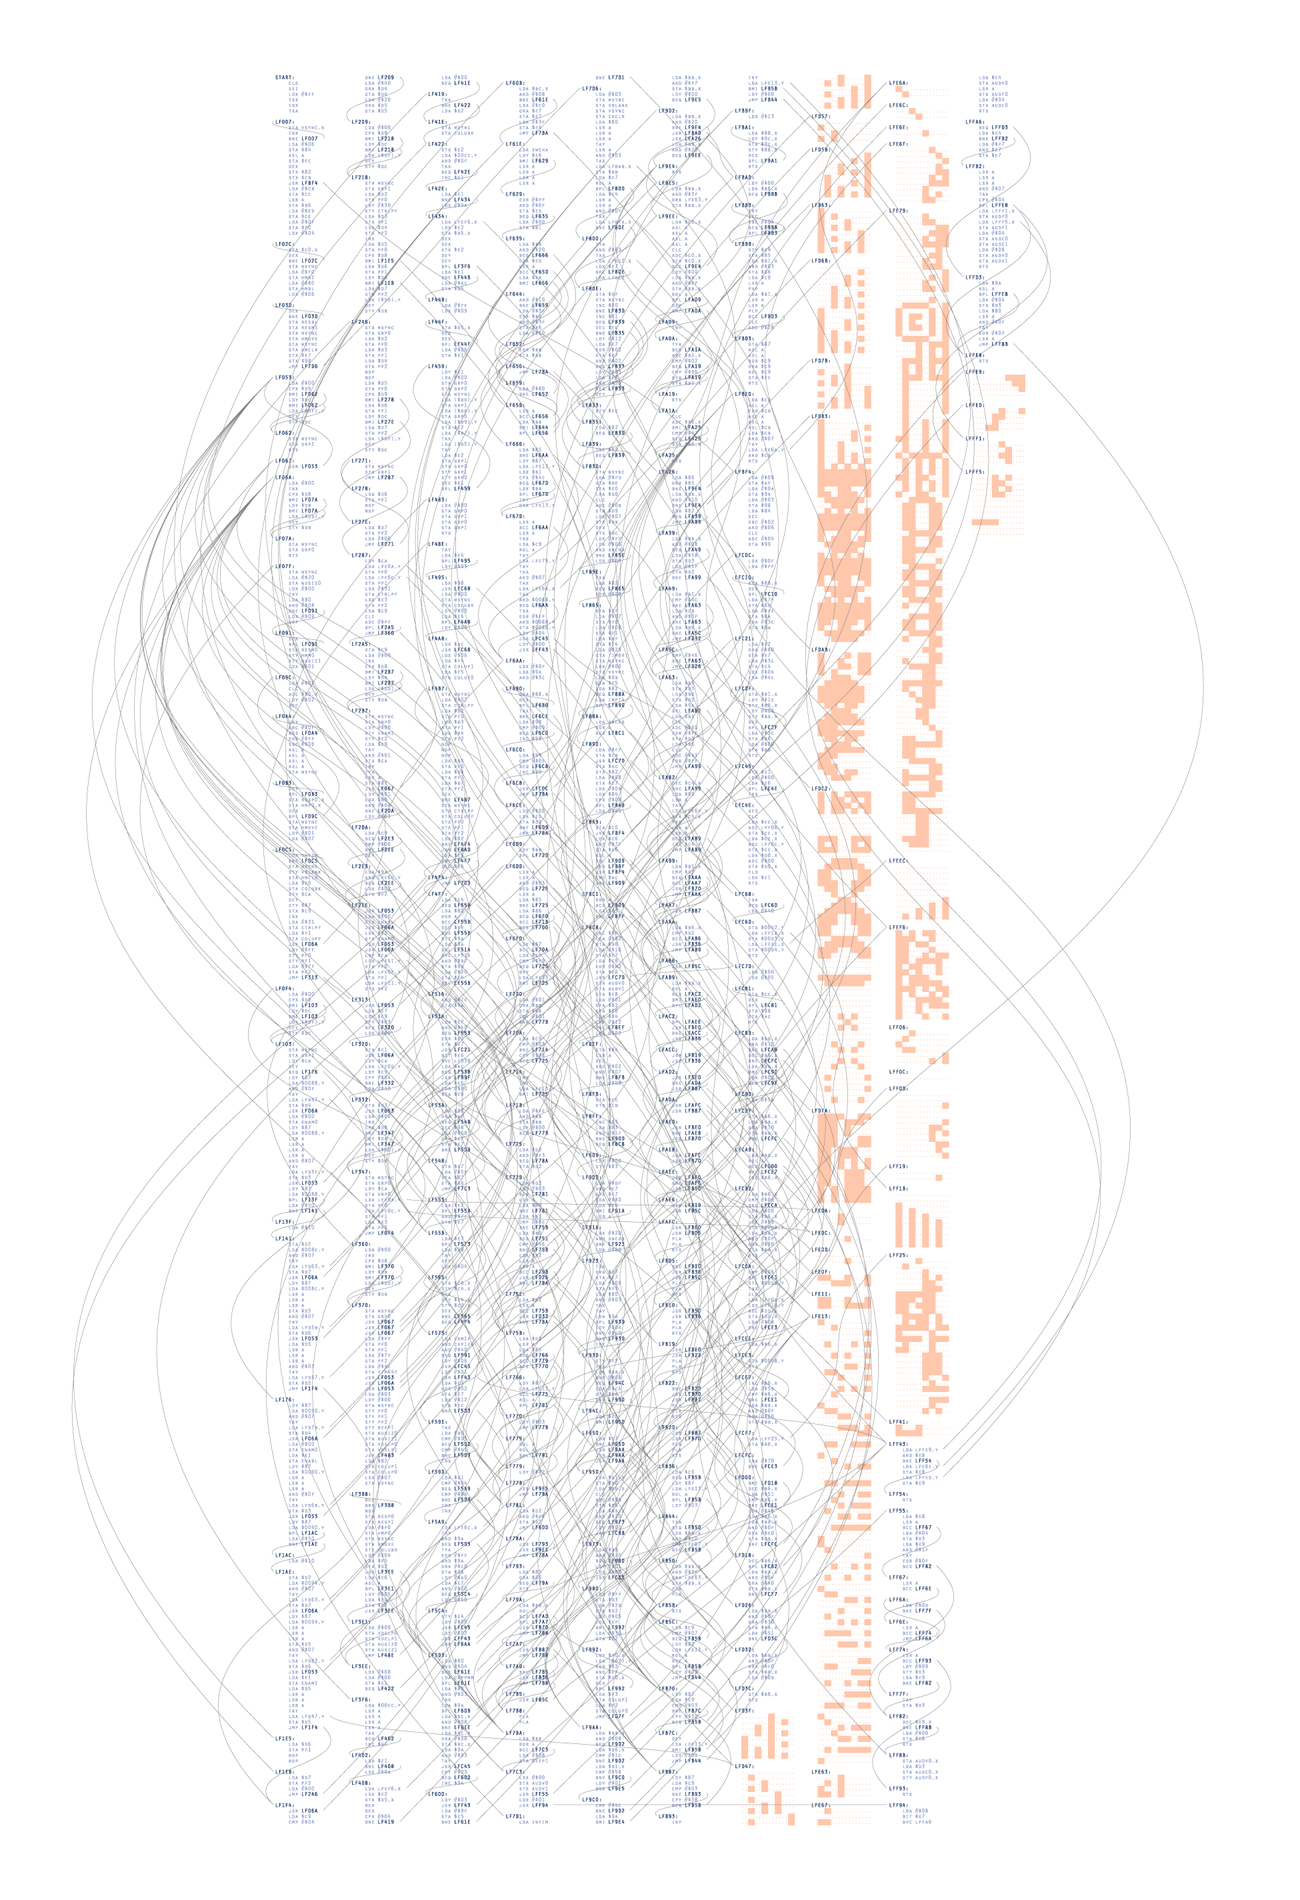
\includegraphics[width=\textwidth,height=\textheight,keepaspectratio]{distellamap_pacman.png}
    \caption{Visualization of the execution of Pac-Man's source code}
    \label{graphic:pacman-visualization}
\end{listing}

Later on, the introduction of multi-core architecture for central processing units in the late 2000s has enabled the broad adoption of multithreading and threaded programming. As a result, source code has transformed from a single non-linear execution to a multiple non-linear process, in which several of these non-linear executions are happening in parallel. Keep tracking of what is executing when on which resource is involved in problems such as \emph{race conditions}, when understanding the scheduling of events (each event every e.g. 1/18000000th of a second on a 3.0 Ghz CPU machine) becomes crucial to ensuring the correct behaviour of the software.

Conversely, the locii of the execution of software creates contributes to those issues. Software can be (dis-)located across multiple files on a single machine, on multiple processes on a single machine, or on multiple processes on multiple machines (on a local-area or wide-area network) \citep{berry_philosophy_2011}. This further fragments the interface to the object of understanding. For instance, the asynchronicity of requesting and processing information from distinct processes is a spatial separation of code which has temporal implications (e.g. due to network latency).

\vspace*{1\baselineskip}
\centerline{\rule{0.13334\linewidth}{.4pt}}
\vspace*{1\baselineskip}

Software, then, exhibits certain properties which make it difficult to understand, from conception to application: software in the real-world involves implementing concepts that lose in translation, interfacing the world through discreete representations, and following the execution of these representations through space and time, as software executes more and more in a distributed and parallel fashion.

% the philosophical enquiries
\subsection{Software ontology} %7k

Now that we've clarified some of what software complexity consists of, we will frame these difficulties in a philosophical context, more specifically the philosophy of technology. We will investigate how these complexities can be seen as stemming from the nature of technology itself, and how this allows us to reconnect it to aesthetic perception. Before moving back to practical inquiries into how specific individuals engage with this nature, this section will help provide a theoretical backdrop, framing technology as a relational practice, complementing other modes of making sense of and taking action on the world. This conceptual framework will start with an investigation into the denomination of software as an \emph{abstract artifact}, followed by an analysis of technology as a specific mode of being, and concluding on how it is related to an aesthetic mode of being.

% first on the abstract artifact - 3.5k
\subsubsection{Software as abstract artifact}

When he coins the phrase \emph{abstract artifact}, Nurbay Irmak addresses software partly as an abstract object, similar in his sense to Platonic entities\footnote{Like Joseph Kosuth's aforementioned trio of chairs..}. Nonetheless, he also grants that software holds spatio-temporal properties \citep{irmak_software_2012}. Indeed, software does need to exist as an implementation, in the form of source code \citep{suber_what_1988}; this implies that software is composed of files, has a beginning (start) and an end (exit), meanwhile also representing ideas of structure and procedure which go beyond these limitations of being written to a disk and having an execution time. Typically, the physical aspects of software (its manifestation as source code) can be changed\footnote{A process called \emph{refactoring}.} without changing any of the ideas expressed by the software\footnote{A phenomenon one can also observe in natural languages, in which one can radically change a syntax without drastically changing the semantics of a sentence.}.

Complementing Irmak, Colburn's phrasing is that of a \emph{concrete abstraction}, an oxymoron which echoes the tensions denoted by the concept of an abstract artifact. 

He grounds these tensions in the distinction between a medium of execution (a—potentially virtual—machine) and a medium of description (source code). He considers that, while any high-level programming language is already the result of layers of abstraction, such language gets reduced to the zeroes and ones input to the central processing unit \citep{colburn_philosophy_2000}. Here, he sees the abstraction provided by languages ultimately bound to the concrete state of being of hardware and binary. And yet, if we follow along along his reasoning, these representations of voltage changes into zeroes and ones are themselves abstractions over yet another concrete, physical event.

Writing on computational artefacts, of which software is a subset, Raymond Turner formalizes this specificity of in a three-way relationship. Namely, abstract artefact A is an implementation in medium M of the definition F. For instance, concerning the medium:

\begin{quote}
    Instead of properties such as \emph{made from carbon fiber}, we have properties such as \emph{constructed from arrays in the Pascal programming language, implemented in Java}. \citep{turner_computational_2018}
\end{quote}

This metaphor provides an accurate but limited account of the place of source code within the definition of software: the Java implementation is itself a definition implemented in a specific bytecode, etc. Nonetheless, source code is that which gives shape to the ideas immanent in software—through a process of concretization—and which hides away the details of the hardware—through abstraction. This metaphor of \emph{abstract artifact} thus helps to clarify the tensions within software, and to locate the specific role of source code within the different moving parts of definition, medium and model.

Recalling that software has a somewhat unique relatoin between its \emph{functional} properties (i.e. purpose that are intended to be achieved through their use) and \emph{structural} ones (physical configuration which are involved in the fullfilment of the functional purpose) \citep{turner_computational_2018}, it remains nonetheless a kind of technology. As such, it also holds some of the specifities of this lineage, into which we can extend our inquiry.

\subsubsection{Software as a relational object} %3.5k

The technological object underwent a first qualitative shift during the European Industrial Revolution, and a second one with the advent of computing technologies. The status of its exact nature is therefore a recent object of inquiry. Here, we will start from Gilbert Simondon's understanding of technology as a \emph{mode}, in order to ultimately contrast it with the \emph{aesthetic mode}.

According to Simondon, the technical object is a relation between multiple structures and the result of a complex operation of various knowledges \citep{simondon_mode_1958}, some scientific, some practical, some social, some material. The technical object is indeed a scientific object, but also a social object and an artistic object at the same time. Differentiated in its various stages (object, individual, system), it is therefore considered as relational, in that its nature changes through its dependance and influence on its environment.

From this relational standpoint, one could complement Bernard Stiegler's statement that technology is a dynamic of organized, but inorganic matter \citep{stiegler_technics_1998}, if we are to consider inorganized matter to include social influences, personal practices, and forms of tacit and explicit knowledges. That is, the ambiguity of the technical object is that it extends beyond itself as an object, entering into a relation with its surrounding environment, including the human individual which makes use of it. Up until the invention of the clock, technology remained bound to practical matter. With the invention of seconds, its action reached into another domain—that of mechanical operation on abstract ideas \citep{mumford_technics_1934}.

The domain of abstract ideas was hitherto reserved to different modes than technology: that of religion and philosophy, and technology holds a particularly interesting relation with these two. According to Simondon, philosophy followed religion as a means of relating to, and making sense of, the abstract such the divine and the ethical. Tracing back the genesis of the technological object, e writes that the technical mode of existence is therefore just another mode through which the human can relate to the world, similar to the religious, the philosophical, and the aesthetic mode\citep{simondon_mode_1958}.

While both technology, religion and philosophy are based on theoretical knowledge, technology is specifically manifested in practice, and while it is manifested in ethics, in religion. Technology is thus seen as the combination of a theory of knowledge and a theory of action. Such a combination has since been extended into the abstract domain, leading to computers, as a form of technology through which \emph{meaning is mechanically realized}.

%TODO add a section on yuk hui here, for the digital objects.

Simondon complements the technical and the religious modes with the aesthetic mode, and as such counter-balances the apparent split between technics and religion by striving for unity and totality, for the balance between the objective and the subjective. Yet, rather than being a monadic unity of a single principle, Simondon considers the aesthetic mode as a unifying a network of relationships, a form of organizing Stiegler's inorganized matter. He further argues that the aesthetic mode goes beyond taste and subjective preference, into a fundamental aspect of the way in which human beings relate to the world around them. An aesthetic object therefore acquires the property of being beautiful by virtue of its relationships, of its connections between the subject and the objective, between one's history and one's perceptions, and the various elements of the world, and the actions of the individual. Finally, the aesthetic thought when related to the technical object consists in preparing the communication between different communities of users, between different perspectives on the world, and different modes of action upon this world. An aesthetic object can therefore be seen as a nexus of relationships found in its environment, echoing how Goodman considers an aesthetic language as way for worldmaking.

Software is therefore a manifestation of technology as both knowledge and action. Furthermore, it also enables ways to act mechanically on knowledge and ideas, an affordance named \emph{epistemic action} by David Kirsh and Paul Maglio \citep{kirsh_distinguishing_1994}. They define epistemic actions as actions which facilitate thinking through a particular situation or environment, rather than having an immediate functional effect on the state of the world. As technology changes the individual's relationship to the world, software does so by being the dynamic notion of a state of a process \citep{rapaport_philosophy_2005}, ever evolving around a fixed structure, and by changing the conceptual understanding of said world. Such examples of world related to the environment in which software exists, e.g. the social environment, or hardware environment, or the environment which has been recreated within software. David M. Berry investigates this encapsulation of world in his \emph{Philosophy of Software}:

\begin{quote}
    The computational device is, in some senses, a container of a universe (as a digital space) which is itself a container for the basic primordial structures which allow further complexification and abstraction towards a notion of world presented to the user. \citep{berry_philosophy_2011}
\end{quote}

Software-as-world is the material implementation of a proposed model, itself derived from a theory. It therefore primarily acts at the level of \emph{episteme}, sometimes even limiting itself to it\footnote{Functional programming languages take pride in the fact that they have no effect on the world around them, being composed exclusively of so-called \emph{pure functions}, and no external side-effects, or input/output considerations}. Paradoxically, it is only through peripherals that software can act as a mechanical technology in the industrial sense of the word.

Along with software's material and theoretical natures (i.e. in contemporary digital computers, it consists of electrons, copper and silicium and of logical notations), another environment remains—that of the intent of the humans programming such software. Since it can be so many things, it might not be exactly clear what a specific piece of software, manifested in source code, is exactly about.

Indeed, thinking through the function of computational artefacts, Turner states that it is \emph{agency} which determines what the function is: and he defines agency as the resolution of the difference between the specification (intent-free, external to the program) and semantic interpretation (intent-rich, internal to the programmer) \citep{turner_computational_2018}. In order to understand a computer program, to understand how it exists in mutliple worlds, and how it represents the world, we need to give it meaning. To make sense of it, a certain amount of interpretation is requiredin relation to that of the computer's—such that the question "what does a Turing machine do?" has \lstinline{n+1} answers. 1 syntactic, and \lstinline{n} semantic (e.g. however many interpretations as there can be human interpreters) \citep{rapaport_philosophy_2005}. In his investigation into what software is, Suber corroborates:

\begin{quote}
    This suggests that, to understand software, we must understand intentions, purposes, goals, or will, which enlarges the problem far more than we originally anticipated. [...] We should not be surprised if human compositions that are meant to make machines do useful work should require us to posit and understand human purposiveness. After all, to distinguish \emph{literature} from noise requires a similar undertaking. \citep{suber_what_1988}
\end{quote}

\vspace*{1\baselineskip}
\centerline{\rule{0.13334\linewidth}{.4pt}}
\vspace*{1\baselineskip}

In conclusion, we've seen that while software can be given the particular status of an \emph{abstract artifact}, these tensions are shared across technological objects. Technology, as a combination of a theory of knowledge and a theory of action, as an interface to the world and a recreation of the world, is furthermore related to other modes of existence—and in particular the aesthetic mode. All of these tensions and paradoxes, from the various levels of existence, the various types of complexities, the different kinds of actions and interpretations that it allows, contribute to the cognitive hurdles encountered when attempting to understanding software.

And yet, programmers, have been understanding software as long as they have been writing and reading it. We now turn to understanding how programmers understand software, through a empirical perspective of the psychology of programming..

\subsection{The psychology of programming} %7k
% the studies

How programmers deal with such a complex object as software has been a research topic which appeared much later than software itself. This field aims at understanding how programmers process code, and with which level of success, and under which conditions. How do they build up their understanding(s), in order to afford appropriate modification, re-use or maintenance of the software? What cognitive abilities do they summon, and what kind of technical apparatuses play a role in this process? Specifically, we will see how hard it is to answer these questions, and how diversity and multiplicity are recurrent patterns in sketching out answers.

Epistemic actions thus contribute to reducing the kinds of complexities involved with software. Concretely, this involves the creation of mental models of the software system with which the indvidual is interacting. In their work on computer-enabled cognitive skills, Kirsh and Maglio develop on the use of epistemic actions:

\begin{quote}
    More precisely, we use the term epistemic action to designate a physical action whose primary function is to improve cognition by:
    \begin{enumerate}
        \item reducing the memory involved in mental computation, that is, space complexity;
        \item reducing the number of steps involved in mental computation, that is, time complexity;
        \item reducing the probability of error of mental computation, that is, unreliability.
    \end{enumerate}
    \citep{kirsh_distinguishing_1994}
\end{quote}

Psychological studies of programming practices have been focused on the identification and analysis of these mental models, as well as on their optimization through experimental devices, and the social behaviour of programmers within a context of practice \citep{weinberg_psychology_1998}.

Mental models, as kinds of internal symbolic representation of an external reality, are a rigorous, personal and conceptual structure. They are related to knowledge, since the construction of accurate and useful mental models through the process of understanding underpins knowledge acquisition. However, mental models need not be correlated with empirical truth, due to their personal nature, but are extensive enough to be described by formal (logical or diagrammatical) means. Mental models can be informed, constructed or further qualified by the use of metaphors, but they are nonetheless more precise than other cognitive structures such as metaphors—a mental model can be seen as a more specific instance of a conceptual structure.

The earliest studies of how computer programmers understand the code they are presented with consisted mostly in pointing out the methodological difficulties in doing so \citep{sheil_psychological_1981,shneiderman_measuring_1977}. This is mainly due to three parameters. First, programming is an intertwined combination of notation, practices, tasks and management, each of which have their own impact on the extent to which a piece of source code is correctly understood, that it is hard to clearly establish the impact of each of these. Second, program comprehension is strongly influenced by practice—the skill level of the programmer therefore also influences experimental conditions. Third, these early studies have found that programmers have organized knowledge bases, if informal. This means that, while programmers demonstrate epistemic mastery, they are limited in their ability to explain the workings of such ability—that is, the constitution and use of their own epistemic models, which she calls knowledge maps.

Shifting to qualitative interviews, rather than quantitative and performative assessments, Marian Petre and Alan Blackwell attempted in their 1992 study to identify these mental models and their uses. They asked 10 expert programmers from North America and Europe to describe the thought process in source code-related problem-solving and design solutions in code. The main conclusion of their study is that, beyond the fact that each programmer had slightly different descriptions of their mental process, there a some commonalities to what is happening in someone's thoughts as they start to design software. The behaviour is dynamic, but controlled; the resolution of that behaviour was also dynamic, with some aspects coming in and out of focus that the will of the programmer, providing more or less uncertainty, level of details and fuzziness on-demand; and those images co-existed with other images, such that one representation could be compared with another representation of a different nature \citep{petre_glimpse_1997}. Finally, while most imagery was non-verbal, all programmers talked about the need to have elements of this imagery labelled at all times, hinting at a relationship between syntax and semantics to be translated into source code. While this study was an investigation into the design of code, before any writing happens, one of the limitations is that it did not investigate the understanding of code, which takes places once the writing has been done (by oneself, or someone else), and the code now needs to be read.

Francoise Détienne, in her study of how computer programmers design and understand programs \citep{detienne_software_2012}, defines the activity of designing and understanding programs in activating \emph{schemas}, mental representations that are abstract enough to encompass a wide use (web servers all share a common schema in terms of dealing with requests and responses), but nonetheless specific enough to be useful (requests and responses are qualitatively different subsets of the broader concept of inputs and outputs). An added complexity to the task of programming comes with the one of the dual nature of the mental models needing to be activated: the computer's actions and responses are comprised of the prescriptive (what the computer should do) to the effective (what the computer actually does). In order to be appropriately dealt with, then, programmers must activate and refine mental models of a program which resolves this tension.

In programming, within a given context—which includes goals and heuristics—, elements are being perceived, processed through existing knowledge schemas in order to extract meaning. Starting from Kintsch and Van Dijk's approach of understanding text \citep{kintsch_model_1978}, Détienne nonetheless highlights some differences with natural language understanding. In program texts, she finds, there is an entanglement of the plan, of the arc, of the tension, which does not happen so often in most of the traditional narrative text. A programmer can jump between lines and files in a non-linear, explorative manner, following the features of computation, rather than textuality. Program texts are also dynamic, procedural texts, which exhibit complex causal relations between states and events, which need to be kept track of in order to resolve the prescriptive/effective discrepancies. Finally, the understanding of program text is first a general one, which only subsequently applies to a particular situation (a fix or an extension needing to be written), while narrative texts tend to focus on specific instances of protagonists, scenes and descriptions, leading to broad thematic appreciation.

Conversely, a similarity in understanding program texts and narrative texts is that the sources of information for understanding either are: the text itself, the individual experience and the broader environment in which the text is located (e.g. technical, social). Building on Chomsky's concepts, the activity of understanding in programming can be seen as understanding the \emph{deep structure} of a text through its \emph{surface structure} \citep{chomsky_aspects_1965}. One of the heuristics deployed to achieve such a goal is looking out for what she calls \emph{beacons}, as thematic organizers which structure the reading and understanding process. For instance, in traditional narrative texts, beacons might be represented by section headings, or the beginning or end of paragraphs. However, one of the questions that her study hasn't answered specificall, how the specific surface structure in programming results in the understanding of the deep structure—in other terms, what is the connection between source code syntax, programmer semantics and program behavior.

Due to its relation to text, syntax and semantics, it has often been assumed by programmers and researchers that reading and writing code is akin to reading and writing natural languag prose. Additional recent research in the cognitive responses to programming tasks, conducted by Ivanova et. al., do not appear to settle the question of whether programming is rather dependent on language processing brain functions, or on functions related to mathematics (which do not rely on the language part of the brain) \citep{ivanova_comprehension_2020}, but contributes empirical evidence to that debate. They conclude that, while language processing might not be one of the essential ways that we process code—excluding the \emph{code is language} hypothesis—, it also does not rely on exclusively mathematical functions. Stimulating in particular the so-called multi-demand system, it seems that programming is a polymorphous activity involving multiple exchanges between different brain functions. What this implies, though, is that neither literature, linguistics nor mathematics should be the only lens through which we look at code.

In a way, then, programming is a sort of fiction, in that the pinpointing of its source of existence is difficult, and in that it affords the experience of imagining contents of which one is not the source, and of which the certainty of isn't defined. Both programming and fiction suggest surface-level guiding points helping the process of constructing mental models as a sort of conceptual representation. It is also something else than fiction, in that it deals with concrete issues and rational problems \footnote{more often than not, a pestering bug}, and that it provides a pragmatic frame for processing representations, in which assumptions stemming from burgeoning mental models can be easily verified or falsified, through the taking of epistemic actions. It might then be appropriate to treat it as such, simultaneously fiction and non-fiction, as knowledge and action, mathetmatic and artistic. Indeed, it is also an artistic activity which, in Goodman's terms, might be seen as \emph{an analysis of [artistic] behavior as a sequence of problem-solving and planning activities."} \citep{goodman_basic_1972}.

Remains the interpretation issue mentioned above: the interpretation of the machine is different from the interpretation of the human, of which there are many, and therefore what also needs to be intepreted is the intent of the author(s). Reading is then akin to constructing a \emph{cognitive cartography}, allowing for an experience to be made intelligible, sensible, and verifiable, and when an experience is made sensible is when it enters the realm of the aesthetic. In a very immediate understanding of aesthetics, we conclude on the role of form in cognition in those psychological studies. One of the focus was on demonstrating the impact that formal arrangement has on program comprehension\citep{oman_typographic_1990,oliveira_systematic_2022}. Spacing, alignment, syntax highlighting and casing are all parameters which have an impact on the readability, and therefore understandability of code. The next section therefore looks at two ways in which meaning can be extracted from intention and source code; this means how individuals use metaphors to communicate complex ideas, and how they use computational tools in order to navigate program texts.

%todo include comparison of color vs. not color coded (or maybe in the IDE section below?)

The fact that software exists between the state of being conceptually designed and materially implemented predates software itself, and can be observed in modern technological developments at large. Furthermore, these complexities are echoed in how programmers evoke their experience of either designing or, comprehending code. They have shown to use multiple cognitive abilities, without being strictly limited to narrative, or mathematic frames of understanding, and making use of notions of scale and focus to disentangle complexity. For the remaining section of this chapter, we will focus on two specific means that contribute to this process of building a mental model of software-as-source code. Based on the reports that programmers use mental images and play with dynamic mental structures to comprehend the functional and structural properties of software; we thus inquire into the role that metaphors play in translating computational concepts into ones which can be grasped by an individual. Conversely, in response to the role of indentation, typography and navigation, we will see how cognition is also distributed in a programmers' tools.

\clearpage

\section{Means of understanding}

Drawing on the ambivalence of software's existence—both concrete and abstract—we now investigate the means deployed to graps software on both of these levels. As we've seen in empirical studies, programmers resort to both conceptual techniques to visualize and grasp a piece of software, along with more practical and technical tools. In this spirit, we will look at the ubiquity of metaphors in computing,  both from users and programmers, and how they act as a cognitive mechanism. We will also look at how cognitive tools can be manifested concretely though the extension of mind through software tools, and particularly on the role of \emph{Integrated Development Environments} (IDEs). This will establish the research ground of the subsequent chapters, in which we establish aesthetics as one of the cognitive tools used by programmers.

\vspace*{1\baselineskip}

\subsection{Metaphors in computation}

\subsubsection{Theoretical background}

This part of the thesis relies on the work of George Lakoff and Mark Johnson, and on that of Paul Ricoeur, due to their requalification of the nature and role of metaphor in the 20th century. While Lakoff and Johnson's approach to the conceptual metaphor will serve a basis to explore metaphors in as a cognitive means across software and narrative, I also argue that Ricoeur's focus on the tension of the \emph{statement} rather than primarily on the \emph{word} will help us better understand some of the aesthetic manifestations and workings of software metaphors. Following a brief overview of their contributions, I examine the various uses of metaphor in software.

%and in literature, touch upon the cognitive turn in literary studies, and conclude the section by the ambiguity of a cognitive account of programming.

We depart here from the most commonly used definition of metaphor: that of labeling one thing in terms of another, thereby granting additional meaning to the subject at hand. Our approach here will also bypass some of the more minute distinctions made between metonymy (in which the two things mentioned are already conceptually closely related), comparison (explicitly assessing differences and similarities between two things, often from a value-based perspective) and synechdoche (representing a whole by a subset), as they all relate to a larger, more contemporary definition of the concept.

Such a definition stems from Lakoff and Johsnon's seminal work through which they develop a theory of conceptual metaphors by highlighting their essential dependence on pre-existing cognitive structures, which we associate with already-understood concepts. The metaphor maps a source domain (made up of cognitive structure(s)) to a target domain. In the process, they extend the field of applicability of metaphors from the strictly literary to the broadly cultural: metaphors work because each of us has some conception of those domains involved in the metaphorical process. Metaphors rely in part on a static understanding, resulting in a fixed meaning from the application of a given source to a given target. Some of these sources are called \emph{schemas}, and are defined enough to not be mistaken for something else, but broad enough to allow for multiple variants of itself to be applied to various targets \citep{lakoff_metaphors_1980}, providing both diversity and reliability. As we will see below, their approach allows us to focus not just on textual objects, but on the vast range of metaphors used also in computing-related environments. Given that the source of the metaphor should be well-grounded, with as little invariablity as possible, in order to qualify a potentially ill-defined target domain, we see how this is a useful mechanism to provide an entrypoint to end users and novice programmers.

Going beyond the role of metaphors manifested in expressions such as \emph{the desktop}, \emph{the mouse}, or \emph{the cloud}, we will explore Lakoff's understanding of the specifically poetic metaphor further below as preliminary work to assess the linguistic component of computing—source code. For now, to complement his broadening of the metaphorical field, we turn to Paul Ricoeur's assessment of it.

Writing in \emph{The Rule of Metaphor}, Ricoeur operates two shifts which will help us better assess not just the inherent complexity of program texts, but the ambivalence of programming languages as well. His first shift regards the locus of the metaphor, which he saw as being limited to the single word—a semiotic element—to the whole sentence—a semantic element \citep{ricoeur_rule_2003}. This operates in parallel with his attention to the \emph{lived} feature of the metaphor, insofar it exists in a broader, vital, experienced context\footnote{Similar to Simondon's characterization of the technological mode as a mode of relations.}. Approaching the metaphor only through words is counterproductive because words refer back to "contextually missing parts"—they are eminently overdetermined, polysemic, and belong to a wider network meaning than a single, one-to-one relationship\footnote{As Ricoeur sees it being considered in the traditional, Aristotelician sense of the term.}. Looking at it from the perspective of the sentence brings this rich network of potential meanings and narrows the scope for interpretation. As we've briefly touched upon in the previous section when reading \lstinline{self_inspect.rb}, all of the evocative meaning of the poem isn't contained exclusively in each token, and the power of the whole is greater than the sum of its parts. % TODO add a reference to the next chapter where we analyze self_inspect.rb

Secondly, Ricoeur inspects a defining aspect of a metaphor by the \emph{tensions} it creates. His analysis builds from the polarities he identifies in discourse between event (time-bound) and meaning (timeless), between individual (subjective, located) and universal (applicable to all) and between sense (definite) and reference (indefinite)\footnote{For the extent to which source code can be considered discourse has been discussed, see: Cox and McLean, \emph{Speaking Code} \citep{cox_speaking_2013}.}. The creative power of the metaphor is its ability to both create and resolve these tensions, to maintain a balance between a literal interpretation, and a metaphorical one—between the immediate and the potential, so to speak. Tying it to the need for language to be fully realized in the lived experience, he poses metaphor as a means to creatively redescribe reality. One of the realities needing to be described is the foreign land of computing.

% As we will be approaching the topic of syntax and semantics in programming languages, we will see that these tensions can be a fertile ground for poetic creation through aesthetic manifestations.

% then the communcation between both
\subsubsection{Metaphors for end-users}

It is interesting to consider that the first metaphor in computing might be concommitant with the first instance of modern computing—the Turing \emph{machine}. While Turing machines are widely understood as being manifested into what we call digital computers (laptops, tablets, smartphones, etc.), and thus definitely within the realm of machines, the Turing machine isn't strictly a machine \emph{per se}. Rather, it is more accurately defined as a mathematical model which in turn defines an abstract machine. Indeed, computers cannot be proved or assumed to be machines, because their terminology comes from logic, textual, or discursive traditions (e.g. reference, statement, names, recursion, etc.) and yet they are still \emph{built} \citep{smith_origin_1998}. Humans can be considered Turing machines (and, in fact, one of the implicit requirements of the Turing machine is that, given enough time and resources, a human should be able to compute anything that the Turing machine can compute), and non-humans can also be considered Turing machines\footnote{See research in biological computing, using DNA and protein to perform computational tasks}. Debates in computer science related to the nature of computing \citep{rapaport_philosophy_2005} have shown that computation is far from being easily reduced to a simple mechnical concern, and the complexity of the concept is perhaps why we ultimately revert to metaphors in order to better grasp them.

Jumping ahead to the 1980s, these uses of metaphors became more widespread and entered public discourse once personal computing became available to ever larger audiences. With the release of the XEROX Star, features of the computer which were until then described as data processing were given a new life in entering the public discourse. The Star was seminal since it introduced technological innovations such as a bitmapped display, a two-button mouse, a window-based display including icons and folders. For instance, the desktop metaphor relies on previous understanding of what a desktop is, and what it is used for in the context of physical office-work; since early personal computers were marketed for business applications (such as the Star), these metaphors built on the broad cognitive structures of the user-base in order to help them make sense of this new tool. Paul DuGay, in his cultural study of the Sony Walkman, makes a similar statement when he describes the Sony Walkman, a never-before-seen compound of technological innovations, in terms of pre-existing, and well-established technologies \citep{gay_doing_2013}. The icon of a floppy disk for writing data to disk, the sound of wrinkled paper for removing data from disk, the designation of a broad network of satellite, underground and undersea communications as a cloud, these are all metaphors which help us make a certain sense of the broad possibilities brought forth by the computing revolution \citep{wyatt_danger_2004}. Even the \emph{clipboard}, presented to the user to copy content across applications, does not believe at all like a real clipboard \citep{barrera_how_2022}.

The work of metaphors takes on an additional dimension when we introduce the concept of interfaces. As permeable membranes which enable (inter)actions between the human and the machine, they are essential insofar as they allow for various kinds of agency, based on different degrees of understanding. Departing from the physically passive posture of the reader towards an active engagement with a dynamic system, interfaces highlight even further the cognitive role of the metaphor. These depictions of things-as-other-things influence the mental model which we build of the computer system we engage in. For instance, the prevalent windows metaphor of our contemporary desktop and laptop environments obfuscates the very concrete action of the CPU (or CPUs, in the case of multi-core architecture) of executing one thing at a time, except at speeds which cannot be intuitively grasped by human perception. Alexander Galloway 's work on interfaces as metaphorical representations suggests a similar concern when he bases it on Jameson's theory of cognitive mapping. While Jameson uses it in a political and historical context, the heuristic is nonetheless useful here: cognitive mapping is the process by which the individual subject situates himself within a vaster, unrepresentable totality, a process that corresponds to the workings of ideology. Substituting ideology with the computer\footnote{The relation between which has been explored by Galloway, Chun, Holmes and others, and is particularly apparent in how an operating system is designated in French: \emph{système d'exploitation}.}, we can see how such a process helps make sense of the unthinkable, of that which is too complex to grasp and therefore must be put into symbols (words, icons, sounds, etc.).

% TODO have a word on interfaces, with galloway, cramer and fuller

Moving away from userland, in which most of these metaphors exist, we now turn to examine the kinds of metaphors that are used by programmers and computer scientists themselves. Since the sensual reality of the computer is that it is a high-frequency vibration of electricity, one of the first steps taken to productively engage with computers is to abstract it away. The word \emph{computer} itself can be considered as an abstraction: originally used to designate the women manually inputting the algorithms in room-scale mainframes, the distinction between the machine and its operator was considered to be unnecessary. The relation between metaphor and abstraction is a complex one, but we can say that metaphorical thought requires abstraction, and that the process of abstraction ultimately implies designating one thing by the name of another (a woman by a machine's, or a machine by a woman's), being able to use it interchangeably, and therefore lowering the cognitive friction inherent to the process of specification, freeing up mental resources to focus on the problem at hand \citep{chun_software_2005}.

This need to get away from the specificities of the machines has been one of the essential drives in the development of programming languages. Since we cannot easily and intuitively deal with binary notation to represent complex concepts, programming helps us deal with this hurdle by presenting things in terms of other things. Most fundamentally, we represent binary signs in terms of English language (e.g. from binary to Assembly). This is, again, by no means a metaphorical process, but rather an encoding process, in which tokens are being separated and parsed into specific values, which are then processed by the CPU as binary signs. Still, this abstraction layer offered by programming languages allowed us to focus on \emph{what} we want to do, rather than on \emph{how} to do it. The metaphorical aspect comes in when the issue of interpretation arises, as the possibility to deal with more complex concepts required us to grasp them in a non-rigorous way, one which would have a one-to-one mapping between concepts. Allen Newell and Herbert A. Simon, in their 1975 Turing Award lecture, offer a good example of symbolic manipulation relates inherently to understanding and interpretation:

\begin{quote}
  In none of [Turing and Church's] systems is there, on the surface, a concept of the symbol as something that \emph{designates}.
\end{quote}

The complement to what he calls the work of Turing and Church as automatic formal symbol manipulation is to be completed by this process of \emph{interpretation}, which they define simply as the ability of a system to designate an expression and to execute it. We encounter here one of the essential qualities of programming languages: the ambivalence of the term \emph{interpretation}. A machine interpretation is clearly different from a human interpretation: in fact, most people understand binary as the system comprised of two numbers, 0 and 1, when really it is intepreted by the computer as a system of two distinct signs (red and blue, Alex and Max, hot and cold, etc.). To assist in the process of human interpretation, metaphors have played a part in helping programmers construct useful mental representations related to computing. These metaphors can go both ways: helping humans understand computing concepts, and to a certain extent, helping computers understand human concepts.

\subsubsection{Programmer-facing metaphors}

Perhaps one of the first metaphors a programmer encounters when learning about the discipline is that which states that the function is like a kitchen recipe. You specify a series of instructions which, given some input ingredients (arguments), result in an output result (return value). The difficulty in explaining, in that context, the need for a \emph{void} keyword to individuals with limited experience and knowledge of how programming works is a good example of the non-straightforwardness of computing concepts. Similarly, the use of the term \emph{server} is conventionally associated and represented as a machine sending back data when asked for it, when really it is nothing but an executed script or process running on said machine. Incidentally, a server is also a style of software architecture, to which we will return later.

Another instance of synbolic use relying on metaphorical interpretation can be found in the word \emph{stream}. Originally designating a flow of water within its bed, it has been gradually accepted as designating a continuous flow of contingent binary signs. \emph{Memory}, in turn, stands for record, and is stripped down of its essentially partial, subjective and fantasized aspects usually highlighted in literary works (perhaps \emph{volatile memory} gets closer to that point). Finally, \emph{objects}, which came to prominence with the rise of object-oriented programming, have only little to do with the physical properties of objects, with no affordance for being traded, for acting as social symbols, for gaining intrinsic value, but rather the word is used as such for highlighting its boundedness, and ability to be manipulated without interfering with other objects.

Most of these designations, stating a thing in terms of another aren't metaphors in the full-blown, poetic sense, but they do hint at the need to represent complex concepts into humanly-graspable terms, what Paul Fishwick calls \emph{text-based aesthetics} \citep{fishwick_aesthetic_2001}. The need for these is only semantic insofar as it allows for an intended interaction with the computer to be carried out successfully—e.g. one has an intuitive understanding that interrupting a stream is an action which might result in incompleteness of the whole. This process of linguistic abstraction doesn't actually require clear definitions for the concepts involved. The example of the terminology in modern so-called cloud computing uses a variety of terms stacked up to each other in what might seem to have no clear \emph{denotative} meaning (e.g. Google Cloud Platform offers \emph{Virtual machine compute instances}), but nonetheless have a clear \emph{operative} meaning (e.g. the thing on which my code runs). This further qualifies the complexity of the sense-making process in dealing with computers: we don't actually need to truly understand what is precisely meant by a particular word, as long as we use it in a way which results in the expected outcome\footnote{See the famous comment in the UNIX source: \emph{You are not expected to understand this}.}.

The reverse process also brings forth issues of conceptual representation through formal symbolic means. The work of early artifical intelligence researchers consists not just in making machines perform intelligent tasks, but also implies that intelligence itself should be clearly and inambiguously represented. The work of Terry Winograd, for instance, was concerned with language processing (intepretation and generation) \citep{winograd_language_1982}. Through his inquiry, he touches on the different ways to represent the concept of language in machine-operational terms, and highlights two possible represenations which would allow a computer to interact meaningfully with language. He considers a \emph{procedural} representation of language, one which is based on algorithms and rules to follow in order generate an accurate linguistic model, and a \emph{declarative} representation of language, which relies on data structures which are then populated in order to create valid sentences. At the beginning of his exposé, he introduces the historically successive metaphors which we have used to build an accurate mental representation of language (language as law, language as biology, language as chemistry, language as mathematics). As such, we also try to present language in other terms than itself in order to make it actionable within a computing environment.

As we've seen, metaphors are implicitly known not to be true in their most literal sense. Max Black in \emph{Models and Metaphors} argues that metaphors are too loose to be useful in analytic philosophy, and therefore too loose for programming languages, heavily based on the analytic tradition. Yet, they still rely heavily on models in order to make human concepts graspable and operation to the computer. These tools deployed during the representational process differ from conventional or poetic metaphors insofar as they can be logically operated upon and therefore empirically verifiable or falsifiable. These models are means through which we aim at taking the conceptual structures on which metaphors also operate, and explicit them in formal symbol systems.

Abstraction, metaphors and symbolic representations are therefore used tools when it comes to understanding some of the structures and objects which constitute computing and software, in terms of trying to represent to ourselves what it is that a computer can and effectively does, and in terms of explaining to the computer what it is we're trying to operate on (from an integer, to a non-ASCII word, to a renewable phone subscription or to human language). Further more, the implication of spatial and visual components in mental models already highlighted by Lakoff and Johnson, and pointed out through the psychology experiments on programmers allow us to turn to metaphors as an architecture of thought \citep{forsythe_cathedrals_1986}, a concept that will be further developed in section XXX.

\vspace*{1\baselineskip}
\centerline{\rule{0.13334\linewidth}{.4pt}}
\vspace*{1\baselineskip}

Metaphors are used as cognitive tools in order to facilitate the construction of mental models of software systems. Following the line of thought traced by Brian Cantell-Smith on his conception of computation as \emph{meaning mechanically realized}, we can also trace the mechanical realization of the metaphor through the interfaces of software tools. This next section thus focuses on how metaphors get reified in tools, and how tools help programmers think.

\subsection{Tools as a cognitive extension} %7k

First, we will be looking at interfaces, and how interfaces in the traditional sense of the term, where it can help with the manipulation of things. This will connect the abstract perspective of the metaphor with the concrete perception of the manipulation.

\subsubsection{Manipulating abstract objects}

As we've seen in the previous sections, metaphors can be embedded within a  particular technical environment in order to allow users to build an effective mental model of what the system is or does, and thus to effectively act in  a way whereby the result of these actions will conform to their intent and expected result (e.g. put a file in the trash to make it disappear).

Specifically, Nielsen and Gentner develop on some challenges that arise when one uses metaphors not just for conceptual understanding, but for further conceptual manipulation. In \emph{The Anti-Mac Interface}, they point out that differences in features between target domain and source domain are inevitable. For instance, a physical pen would be able to mark up any part of a physical form, whereas a tool symbolize by a pen icon on a document editing software might restrict an average user to specific fields on the form. Their study leads to assess alternatives to one kind of interface\footnote{The one designed by Apple for the Macintosh in the 1990s.}, in order to highlight how a computer system with similar capabilities (both being Turing-complete machines), could differ in (a) the assumptions made about the intent of the user, (b) the assumptions made about the expertise level of the user and (c) the means presented to the user in order to have them fulfill their intent \citep{gentner_antimac_1996}.

Interfaces decide on the way the abstract entities are delimited and represented: through icons or text, with grouped actions or granular actions, weak object-orientation or strong object-orientation, etc. By affecting their manipulation, via their affordances, they also affect the kinds of epistemic actions that can be performed in order to complete the mental model of the objects at hand. For instance, Ken Perlin's \emph{Chalktalk} focuses on freehand input creation and programmatic input modification in order to explore properties and relations of mathematical objects (e.g. geometrical shapes, vectors, matrices) \citep{perlin_chalktalk_2022}, while Brett Victor's \emph{Tangled} focuses in a very sparse textual representation of a dynamic numerical model. The epistemic actions taken within this sysmte thus consists in manipulating the numbers presented in the text result in the modification of the text based on these numbers \citep{victor_tangle_2011,victor_explorable_2011}.

Digital interfaces therefore represent, but also aim to disappear from representation: that is, they aim at providing as direct access as possible to the underlying abstract entities hosted on and performed by the computer.

\subsubsection{Manipulating source code}

The kind of dedicated tool used to deal with source code is called \emph{Integrated Development Environment} (IDE), and covers multiple features to support software writing, reading, versioning and executing. With a specific set of features developing over time, and catered to the needs and practices of programmers, its integral part in software development is such that this tool can be considered an integral part of an extended cognitive process.

One of the first interfaces for writing computer code included the text editor called \emph{EMACS} (an acronym for \emph{Editor MACroS}), with a first version released in 1976. Containing tens of thousands of commands to be input by the programmer at the surface-level in order to affect the deeper level of the computing system, \emph{EMACS} allows for remote access of files, modeful and non-linear editing, as well as buffer-based manipulation \citep{greenberg_multics_1996}, also present in its competitor, \emph{Vim}. This use of tools is, at this point, to design an interfaced system which allows for the almost real-time manipulation of digitized objects (e.g. a paragraph).

While software such as \emph{EMACS} and \emph{Vim} are mostly focused on productivity of text-editing, other environments such as \emph{Turbo Pascal} or \emph{Maestro I} focused specifically on software development tasks in a particular programming language in software such as the Apple WorkShop (1985) \citep{west_macintosh_1987}, or the Squeak system for the Smallktalk programming language \citep{ingalls_back_1997}. The idea is to integrat the various tasks of software development (such as linking, compiling, debugging, block editing and refactoring) into one software, allowing the programmer to switch seamlessly from one task to another, or allowing a task to run in parallel to another task (e.g. indexing and editing).

Throughout this evolution, and with the development of more powerful hardware, IDEs started to develop more elaborated user-interfaces, involving more traditional concepts of aesthetics (such as shape, color, balance, distance, symmetry). IDEs attempt to solve some of the mental operations performed by programmers as they engage with source code. These, mentioned in the previous section, include as chunking, tracing, detecting beacons, and organizing the code space. One specific technical feature, syntax highlighting, shows how a technical system with primarily aesthetic consequences influence \emph{understandability}.

Understanding the source code is impacted both by \emph{legibility} (concerning syntax, and whether you can quickly visually scan the text and determine the main parts of the text, from blocks to words themselves) and \emph{readability} (concerning semantics, whether you know the meaning of the words, and their role in the group) \citep{oliveira_evaluating_2020}. Indeed, the way that the presentation of source code can be modified through extensive customization has been the object of research, and has shown that understanding is indeed impacted by presentation \citep{jacques_understanding_2015}.

This move from legibility (clear syntax) to readability (clear semantics) is what can be called \emph{fluency}. Fluency is, in part, the process of building mental structures that disappear in the interpretation of the representations. The letters and words of a sentence are experienced as meaning rather than markings, the tennis racquet or keyboard becomes an extension of one's body, and so forth. Well-functioning interfaces are thus interfaces which disappear from the cognitive process of their user, allowing them to focus on ends, rather than on means \citep{galloway_interface_2012}, leading to what Paul A. Fishwick has coined \emph{aesthetic programming}, an approach of how attention paid to the representation of code in sensory ways results in better grasping of the metaphors at play in code.

The automation of tooling and workflow increased in software such as Eclipse, IntelliJ, NetBeans, WebStorm Visual Studio Code\footnote{With which this thesis is written.} has led to further entanglements of technology and appearance. One of these is the use of automated styleguides. The evolution of software engineering, from the individual programmer implementing ad hoc and personal solutions to a group of programmers coordinating across time and space to build and maintain large, distributed pieces of software, brought the necessity to harmonize and standardize how code is written—style guides started to be published to normalize the visual aspect of source code. Furthermore, due to their existence within a computational environment, IDEs include software which automatically stylizes code. These, called \emph{linters}, are programs which analyzes the source code being written in order to flag suspicious writing (which could either be suspicious from a functional perspective, or from a stylistic perspective). They act as a sort of \emph{intermediary object}, insofar as they assist individuals in the process of creating another object \citep{jeantet_objets_1998}.

% TODO show figure of formatted code vs. un-formatted code

The problem of style is a problem framed by Georg Simmel's statement regarding the observation that \emph{the practical existence of humanity is absorbed in the struggle between individuality and generality} \citep{simmel_problem_1991}. Simmel's investigation of the topic, which will serve as the foundation for our definition of style, focuses on the dichotomy between works of fine art and mass-produced works of applied arts. Indeed, Simmel draws a distinction between the former, as indiosyncratic objects displaying the subjectivity of its maker, and the latter, as industrially produced and replicated, in which the copy cannot be told apart from the original. The work of fine art, according to him, is \emph{a world unto itself, is its own end, symbolizing by its very frame that it refuses any participation in the movements of a practical life beyond itself}, while the work of applied arts only exists beyond this individuality, first and foremost as a practical object. As these two kinds of work exist at the opposite extremes of a single continuum, we can insert a third approach: that of the crafted object, as a repeated display of its maker's subjectivity, destined for active use rather than passive contemplation. So while style can be seen as a general principle which either mixes with, replaces or displaces individuality, style in programming doesn't stand neatly at either extreme. It involves individual preferences, but also transitions through the objective via such intermediary objects that are linters.

Therefore, automatic tools are also integrated at the surface-level (indentation, line breaks, etc.) but also with consequences at the deep-level, by facilitating human reasoning about these, and by ensuring, to a certain extent, machine readability and execution. In this case, we witness how computer-aided software engineering in the form of IDEs can be both considered as traditional interfaces (surface representation affording direct interfaction) as well as mental interface (formal arrangements whose aim is to facilitate direct engagement with the conceptual structures that it represents, and with the ultimate goal of no long being noticeable). Perception and comprehension of source code is therefore more and more entangled with its automated representation.

\subsubsection{Extended cognition}

There is a long history of computer-mediated knowledge-management, one that finds its roots in the pre-computer era. For instance, the work of the encyclopedists, and scientists in seventeenth-century europe approached knowledge as something which could, and should be rationalized, organized and classified in order to be retrievable, comparable, and actionable \citep{sack_software_2019}. Scholars such as Roland Barthes, Jacques Derrida or Umberto Eco had specific knowledge-management techniques in order to let them focus on the arguments and ideas at hand, rather than on smaller organizational details, through the use of index cards. Perhaps, as Bernard Stiegler argued, technology itself is already a prosthesis for memory \citep{wilken_card_2010}, an external storage which offloads the cognitive burden of having to remember things.

This approach was taken to another level with the emergence of the computer. Laying out his vision for a \emph{Man-Computer Symbiosis}, J.C.R. Licklider, project leader of what would become the Internet and trained psychologist, emphasized information management. He saw the computer as a means to "augment the human intellect by freeing it from mundane tasks" \citep{licklider_mancomputer_1960}. By being able to delegate mundane tasks, one could therefore focus on the most cognition-intensive tasks at hand. While improving speed and memory of contemporary hardware has supported Licklider's perspective a single limitation that he pointed out in the 1950s remains: the problem of language.

What is it that we want to accomplish, and how do we want to accomplish it, are complex questions for a computer to process. The subtleties of language, as highlighted at the beginning of this chapter, result in some ambiguities which is not the preferred mode of working of a logical arithmetic machine. If machines can help us think, there are therefore some aspects of that thinking which cannot cannot easily be translated in the computer's native terms, and the work of interface designers and tool constructors has therefore been to automate most of what can be automated away, and faciltate the more mundane, yet complex if done by hand, tasks done a by a programmer\footnote{Such as batch refactoring, or updating dependency versions.}. Software tools are therefore used to think and explore concepts, by supporting epistemic actions in various modalities \citep{victor_humane_2014}.

The computer therefore supports epistemic actions through its use of metaphors (to establish a fundamental base of knowledge) and of actions (to probe and refine the validity of those metaphors) to build a mental model of the problem domain. In the case of IDEs, the problem domain is the source code, and these interfaces, by allowing means of scanning and navigating the source code, are part of what Simon Penny calls, after Clark and Chalmers, \emph{extended cognition} \citep{penny_making_2019}. Extended cognition posits that our thinking happens not only in our brains, but is also located in the tools we use to investigate reality and to deduce a conceptual model of this reality based on empirical results. IDEs are a specific manifestation of embodied cognition, actively helping the programmer to define, reason about, and explorer a code base. The means of taking epistemic action, then, are also factors in contributing to our understanding of the object at hand (here, source code). In this spirit, David Rokeby goes as far as qualifying the computer as a \emph{prosthetic organ for philosophy}, insofar as it helps him formulate accurate mental models as he interacts with them through computer interfaces.

\vspace*{1\baselineskip}

Programmers face the complexity of software on a daily basis, and therefore use specific cognitive tools to help them. While our overall argument here is that aesthetics is one of those cognitive tools, we focused on this section on two different, yet widely used kinds: the metaphor and the integrated development environment.

We pointed out the role that metaphors play in creating connections between pre-existing knowledge and current knowledge, building connections between both in order to implicitly establish some knowledge of the target domain. Presented to end-users, metaphors are also used by programmers at a different level, helping them grasp concepts (e.g. memory, objects, package) without having to bother with details. As we will see in the following chapters, metaphors are also used by programmers in the source code they write in order to elicit this ease of comprehension for their readers.

Concurrently, programmers also rely on specific software tools, in order to facilitate the scanning and the exploring of source code files, while running mundane tasks which should not require particular programmer attention, such as linking or refactoring. The use of software to understand software is indeed paradoxical, but nonetheless participates in extended cognition; the means which we use to reason about problems affect, to a certain extent, the quality of this reasoning.

\vspace*{1\baselineskip}
\centerline{\rule{0.13334\linewidth}{.4pt}}
\vspace*{1\baselineskip}

\begin{quote}
    Code is therefore technical and social, and material and symbolic simultaneously. Rather, code needs to be approached in its multiplicity, that is, as a literature, a mechanism, a spatial form (organization), and as a repository of social norms, values, patterns and processes. \citep{berry_philosophy_2011}
\end{quote}

This chapter has shown that software is a complex object, an \emph{abstract artifact}, existing at multiple levels, and in multiple dimensions. Programmers therefore need to deal with this complexity and deploy multiple techniques to do so. Psychology studies, investigating how programmers think, have pointed out several interesting findings. First, reading and understanding source code is not an activity which relies exclusively on the part of the brain which reads natural language, nor on the part which does mathematical operations. Second, the reasoning style is multimodal, yet spatial; programmers report working and thinking at multiple levels of scale, represent parts of code as existing closer or further from one another, in non-linear space. Third, the form affects the content. That is, the way that code is spatially and typographically laid out helps, to a certain, with the understanding of said code, without affecting expertise levels, or guaranteeing success.

In order to deal with this complexity, some of the means deployed to understand and grasp computers and computational processes are both linguistic and technical. Linguistic, because computer usage is riddled with metaphors which facilitate the grasping of what the presented entities are and do. These metaphors do not only focus on the end-users, but are also used by programmers themselves. Technical, because the writing and reading of code has relied historically more and more on software which allows programmers to perform tasks specific to source code, in a seamless manner\footnote{Using, for instance, macros or keyboard shortcuts.}.

In the next chapter, we turn to the meeting point of the linguistic and the technical, and to what are yet another hybrid type of interface to source code—programming languages. This exploration will show what status they have in relation to source code, and what kind of aesthetic manifestations they support.


\bibliographystyle{./apa-good.bst}
\bibliography{thesis.bib}

\end{document}